\PassOptionsToPackage{unicode=true}{hyperref} % options for packages loaded elsewhere
\PassOptionsToPackage{hyphens}{url}
%
\documentclass[]{book}
\usepackage{lmodern}
\usepackage{amssymb,amsmath}
\usepackage{ifxetex,ifluatex}
\usepackage{fixltx2e} % provides \textsubscript
\ifnum 0\ifxetex 1\fi\ifluatex 1\fi=0 % if pdftex
  \usepackage[T1]{fontenc}
  \usepackage[utf8]{inputenc}
  \usepackage{textcomp} % provides euro and other symbols
\else % if luatex or xelatex
  \usepackage{unicode-math}
  \defaultfontfeatures{Ligatures=TeX,Scale=MatchLowercase}
\fi
% use upquote if available, for straight quotes in verbatim environments
\IfFileExists{upquote.sty}{\usepackage{upquote}}{}
% use microtype if available
\IfFileExists{microtype.sty}{%
\usepackage[]{microtype}
\UseMicrotypeSet[protrusion]{basicmath} % disable protrusion for tt fonts
}{}
\IfFileExists{parskip.sty}{%
\usepackage{parskip}
}{% else
\setlength{\parindent}{0pt}
\setlength{\parskip}{6pt plus 2pt minus 1pt}
}
\usepackage{hyperref}
\hypersetup{
            pdftitle={Insights from Data Companion},
            pdfauthor={Owen Petchey, Andrew Beckerman, Natalie Cooper, Dylan Childs},
            pdfborder={0 0 0},
            breaklinks=true}
\urlstyle{same}  % don't use monospace font for urls
\usepackage{color}
\usepackage{fancyvrb}
\newcommand{\VerbBar}{|}
\newcommand{\VERB}{\Verb[commandchars=\\\{\}]}
\DefineVerbatimEnvironment{Highlighting}{Verbatim}{commandchars=\\\{\}}
% Add ',fontsize=\small' for more characters per line
\usepackage{framed}
\definecolor{shadecolor}{RGB}{248,248,248}
\newenvironment{Shaded}{\begin{snugshade}}{\end{snugshade}}
\newcommand{\AlertTok}[1]{\textcolor[rgb]{0.94,0.16,0.16}{#1}}
\newcommand{\AnnotationTok}[1]{\textcolor[rgb]{0.56,0.35,0.01}{\textbf{\textit{#1}}}}
\newcommand{\AttributeTok}[1]{\textcolor[rgb]{0.77,0.63,0.00}{#1}}
\newcommand{\BaseNTok}[1]{\textcolor[rgb]{0.00,0.00,0.81}{#1}}
\newcommand{\BuiltInTok}[1]{#1}
\newcommand{\CharTok}[1]{\textcolor[rgb]{0.31,0.60,0.02}{#1}}
\newcommand{\CommentTok}[1]{\textcolor[rgb]{0.56,0.35,0.01}{\textit{#1}}}
\newcommand{\CommentVarTok}[1]{\textcolor[rgb]{0.56,0.35,0.01}{\textbf{\textit{#1}}}}
\newcommand{\ConstantTok}[1]{\textcolor[rgb]{0.00,0.00,0.00}{#1}}
\newcommand{\ControlFlowTok}[1]{\textcolor[rgb]{0.13,0.29,0.53}{\textbf{#1}}}
\newcommand{\DataTypeTok}[1]{\textcolor[rgb]{0.13,0.29,0.53}{#1}}
\newcommand{\DecValTok}[1]{\textcolor[rgb]{0.00,0.00,0.81}{#1}}
\newcommand{\DocumentationTok}[1]{\textcolor[rgb]{0.56,0.35,0.01}{\textbf{\textit{#1}}}}
\newcommand{\ErrorTok}[1]{\textcolor[rgb]{0.64,0.00,0.00}{\textbf{#1}}}
\newcommand{\ExtensionTok}[1]{#1}
\newcommand{\FloatTok}[1]{\textcolor[rgb]{0.00,0.00,0.81}{#1}}
\newcommand{\FunctionTok}[1]{\textcolor[rgb]{0.00,0.00,0.00}{#1}}
\newcommand{\ImportTok}[1]{#1}
\newcommand{\InformationTok}[1]{\textcolor[rgb]{0.56,0.35,0.01}{\textbf{\textit{#1}}}}
\newcommand{\KeywordTok}[1]{\textcolor[rgb]{0.13,0.29,0.53}{\textbf{#1}}}
\newcommand{\NormalTok}[1]{#1}
\newcommand{\OperatorTok}[1]{\textcolor[rgb]{0.81,0.36,0.00}{\textbf{#1}}}
\newcommand{\OtherTok}[1]{\textcolor[rgb]{0.56,0.35,0.01}{#1}}
\newcommand{\PreprocessorTok}[1]{\textcolor[rgb]{0.56,0.35,0.01}{\textit{#1}}}
\newcommand{\RegionMarkerTok}[1]{#1}
\newcommand{\SpecialCharTok}[1]{\textcolor[rgb]{0.00,0.00,0.00}{#1}}
\newcommand{\SpecialStringTok}[1]{\textcolor[rgb]{0.31,0.60,0.02}{#1}}
\newcommand{\StringTok}[1]{\textcolor[rgb]{0.31,0.60,0.02}{#1}}
\newcommand{\VariableTok}[1]{\textcolor[rgb]{0.00,0.00,0.00}{#1}}
\newcommand{\VerbatimStringTok}[1]{\textcolor[rgb]{0.31,0.60,0.02}{#1}}
\newcommand{\WarningTok}[1]{\textcolor[rgb]{0.56,0.35,0.01}{\textbf{\textit{#1}}}}
\usepackage{longtable,booktabs}
% Fix footnotes in tables (requires footnote package)
\IfFileExists{footnote.sty}{\usepackage{footnote}\makesavenoteenv{longtable}}{}
\setlength{\emergencystretch}{3em}  % prevent overfull lines
\providecommand{\tightlist}{%
  \setlength{\itemsep}{0pt}\setlength{\parskip}{0pt}}
\setcounter{secnumdepth}{5}
% Redefines (sub)paragraphs to behave more like sections
\ifx\paragraph\undefined\else
\let\oldparagraph\paragraph
\renewcommand{\paragraph}[1]{\oldparagraph{#1}\mbox{}}
\fi
\ifx\subparagraph\undefined\else
\let\oldsubparagraph\subparagraph
\renewcommand{\subparagraph}[1]{\oldsubparagraph{#1}\mbox{}}
\fi

% set default figure placement to htbp
\makeatletter
\def\fps@figure{htbp}
\makeatother

\usepackage{booktabs}
\usepackage{longtable}
\usepackage[bf,singlelinecheck=off]{caption}


\usepackage{framed,color}
\definecolor{shadecolor}{RGB}{248,248,248}

\renewcommand{\textfraction}{0.05}
\renewcommand{\topfraction}{0.8}
\renewcommand{\bottomfraction}{0.8}
\renewcommand{\floatpagefraction}{0.75}

\renewenvironment{quote}{\begin{VF}}{\end{VF}}
\let\oldhref\href
\renewcommand{\href}[2]{#2\footnote{\url{#1}}}

\ifxetex
  \usepackage{letltxmacro}
  \setlength{\XeTeXLinkMargin}{1pt}
  \LetLtxMacro\SavedIncludeGraphics\includegraphics
  \def\includegraphics#1#{% #1 catches optional stuff (star/opt. arg.)
    \IncludeGraphicsAux{#1}%
  }%
  \newcommand*{\IncludeGraphicsAux}[2]{%
    \XeTeXLinkBox{%
      \SavedIncludeGraphics#1{#2}%
    }%
  }%
\fi

\makeatletter
\newenvironment{kframe}{%
\medskip{}
\setlength{\fboxsep}{.8em}
 \def\at@end@of@kframe{}%
 \ifinner\ifhmode%
  \def\at@end@of@kframe{\end{minipage}}%
  \begin{minipage}{\columnwidth}%
 \fi\fi%
 \def\FrameCommand##1{\hskip\@totalleftmargin \hskip-\fboxsep
 \colorbox{shadecolor}{##1}\hskip-\fboxsep
     % There is no \\@totalrightmargin, so:
     \hskip-\linewidth \hskip-\@totalleftmargin \hskip\columnwidth}%
 \MakeFramed {\advance\hsize-\width
   \@totalleftmargin\z@ \linewidth\hsize
   \@setminipage}}%
 {\par\unskip\endMakeFramed%
 \at@end@of@kframe}
\makeatother

\makeatletter
\@ifundefined{Shaded}{
}{\renewenvironment{Shaded}{\begin{kframe}}{\end{kframe}}}
\makeatother

\newenvironment{rmdblock}[1]
  {
  \begin{itemize}
  \renewcommand{\labelitemi}{
    \raisebox{-.7\height}[0pt][0pt]{
      {\setkeys{Gin}{width=3em,keepaspectratio}\includegraphics{images/#1}}
    }
  }
  \setlength{\fboxsep}{1em}
  \begin{kframe}
  \item
  }
  {
  \end{kframe}
  \end{itemize}
  }
\newenvironment{rmdnote}
  {\begin{rmdblock}{note}}
  {\end{rmdblock}}
\newenvironment{rmdcaution}
  {\begin{rmdblock}{caution}}
  {\end{rmdblock}}
\newenvironment{rmdimportant}
  {\begin{rmdblock}{important}}
  {\end{rmdblock}}
\newenvironment{rmdtip}
  {\begin{rmdblock}{tip}}
  {\end{rmdblock}}
\newenvironment{rmdwarning}
  {\begin{rmdblock}{warning}}
  {\end{rmdblock}}
\newenvironment{action}
  {\begin{rmdblock}{action}}
  {\end{rmdblock}}
\newenvironment{warning}
  {\begin{rmdblock}{warning}}
  {\end{rmdblock}}
\newenvironment{info}
  {\begin{rmdblock}{info}}
  {\end{rmdblock}}
\newenvironment{efficiency}
  {\begin{rmdblock}{efficiency}}
  {\end{rmdblock}}
\newenvironment{safety}
  {\begin{rmdblock}{safety}}
  {\end{rmdblock}}
\newenvironment{reliability}
  {\begin{rmdblock}{reliability}}
  {\end{rmdblock}}

\usepackage{makeidx}
\makeindex

\urlstyle{tt}

\usepackage{amsthm}
\makeatletter
\def\thm@space@setup{%
  \thm@preskip=8pt plus 2pt minus 4pt
  \thm@postskip=\thm@preskip
}
\makeatother

\frontmatter
\usepackage[]{natbib}
\bibliographystyle{apalike}

\title{Insights from Data Companion}
\author{Owen Petchey, Andrew Beckerman, Natalie Cooper, Dylan Childs}
\date{2020-01-02}

\begin{document}
\maketitle


%\cleardoublepage\newpage\thispagestyle{empty}\null
%\cleardoublepage\newpage\thispagestyle{empty}\null
%\cleardoublepage\newpage
%\thispagestyle{empty}
%\begin{center}
%\includegraphics{images/dedication.pdf}
%\end{center}

%\setlength{\abovedisplayskip}{-5pt}
%\setlength{\abovedisplayshortskip}{-5pt}

{
\setcounter{tocdepth}{1}
\tableofcontents
}
\hypertarget{introduction}{%
\chapter{Introduction}\label{introduction}}

\begin{Shaded}
\begin{Highlighting}[]
\NormalTok{knitr}\OperatorTok{::}\NormalTok{opts_chunk}\OperatorTok{$}\KeywordTok{set}\NormalTok{(}\DataTypeTok{cache =} \OtherTok{FALSE}\NormalTok{)}
\end{Highlighting}
\end{Shaded}

\emph{Welcome!}

\{\{\textless{} youtube EHLLmEcqRlk \textgreater{}\}\}

\hypertarget{introduction-1}{%
\section{Introduction}\label{introduction-1}}

The \href{hyperlink\%20to\%20pdf\%20of\%20Preface?}{preface} of \emph{Insights} informs about features of the book, such as its aims, content, structure, intended readership, and content that it does not include. Some of the text in the Preface may come across as a sales pitch (it probably is), but it also aims to make prospective readers clear about what they will find in \emph{Insights} and why. Read the preface and answer \href{insightsfromdata.org}{questions here (directs to a different website)}, directly concerning the content of the Preface, might also help that understanding.

Here you will find the additional information mentioned in the book:

\begin{itemize}
\tightlist
\item
  \href{link\%20to\%20other\%20web\%20site}{Questions and exercises (on a different web site)} with instant feedback that go alongside the material in the book. Use the questions and exercises to check, consolidate, and further your understanding of the material in the book.
\item
  One or two \protect\hyperlink{more-case-studies}{additional case studies}, with exercises and questions .
\item
  Links to the \protect\hyperlink{datasets}{datasets} used in the three case studies in the book.
\item
  \protect\hyperlink{live-data-demo}{Details of a live data analysis demonstration} we often use in our introductory undergraduate classes.
\item
  A list of \protect\hyperlink{more-case-studies}{additional case studies/datasets} that you might practice with (students), or add to your class (instructors).
\item
  A list of \protect\hyperlink{related-books}{Related Books and further reading}.
\end{itemize}

\hypertarget{workflowchecklist}{%
\section{Workflow/checklist}\label{workflowchecklist}}

Refer to this post: 2019-03-14-workflow-checklist-for-data-analysis

\hypertarget{r-project-setup}{%
\section{R-project setup}\label{r-project-setup}}

Here are the ready made empty folders and Rproject files (compressed in a zip file you need to unzip -- \{\{\% staticref ``files/Insights\_projects.zip'' ``newtab'' \%\}\}Insights\_projects.zip\{\{\% /staticref \%\}\}) mentioned in \emph{Insights} (the book) section \emph{R-Projects, the best thing since sliced bread.}

\hypertarget{for-instructors}{%
\section{For instructors}\label{for-instructors}}

Perhaps add the ``Notes/ideas for instructors section from the book Preface.''

\hypertarget{live-data-demo}{%
\subsection{Live data analysis demonstration}\label{live-data-demo}}

In the first class of the first week of an \emph{Introduction to Data Analysis} course, we lead a \emph{live data analysis demonstration}. Within one hour we go from question to answer, including collection of some data about each of the students. We believe this demonstration helps students connect with the importance and fun of the content of the course. A walkthrough of the live data demonstration is provided as an \{\{\% staticref ``files/live\_data\_demo.Rmarkdown'' ``newtab'' \%\}\}Rmarkdown file\{\{\% /staticref \%\}\} and as \{\{\% staticref ``files/live\_data\_demo.html'' ``newtab'' \%\}\}html\{\{\% /staticref \%\}\} rendered from the rmarkdown.

\hypertarget{datasets}{%
\section{Datasets}\label{datasets}}

Here are the datasets you will need in order to work along with the three case studies in \emph{Insights}:

\begin{itemize}
\item
  \textbf{Case Study 1 (bat diets)} is about what bats eat and in it we work the data from the published study: \emph{Female dietary bias towards large migratory moths in the European free-tailed bat (Tadarida teniotis)}, by Mata and colleagues in 2016 in the journal \emph{Biology Letters} \href{http://rsbl.royalsocietypublishing.org/content/12/3/20150988}{paper on Biology Letters website}. You must get the dataset from the online data repository in which the researchers deposited it. Get the \texttt{dataset\_Mata.et.al.2016.xlsx} from the folder \textbf{Diet analysis dataset} from the \href{https://doi.org/10.5061/dryad.m8t72.2}{dryad repository}. Please make sure you get the file from version 2 of the dryad data publication. The dataset is stored on dryad in Excel format.
\item
  \textbf{Case Study 2 (prey diversity)} is about the hypotheses that more pathways of energy flow into a predator (i.e.~more prey species) stabilise the predator population dynamics (\href{https://besjournals.onlinelibrary.wiley.com/doi/abs/10.1046/j.1365-2656.2000.00446.x}{the article about case study 2 is published here}). Get the data the data file \texttt{dileptus\ expt\ data.csv} from the \href{https://datadryad.org/resource/doi:10.5061/dryad.7h62c8t.2}{dryad repository} associated with the publication about the data (make sure you get version 2 of the dataset).
\item
  \textbf{Case Study 3 (dietary diversty and polity)} is about whether the diversity of food available to the population of a country is associated with the political system of that country. It requires three datasets:

  \begin{itemize}
  \tightlist
  \item
    A dataset containing information about country's political system. You can acquire the full dataset from \href{http://www.systemicpeace.org/inscrdata.html}{this web page of the Center for Systemic Peace}. Scroll down to the section \emph{Polity IV: Regime Authority Characteristics and Transitions Datasets} and click on the \emph{Excel Series} link to the right of the \emph{Polity IV Annual Time-Series, 1800-2017} box.
  \item
    A dataset of food available in countries (FAO food balance sheet data) from the \href{http://www.fao.org/faostat/en/\#data/FBS/metadata}{FAO website}. The datafile could get is called \texttt{FoodBalanceSheets\_E\_All\_Data.csv} and is 206MB. You can, as mentioned in the book, opt for the trimmed-down version of the dataset that we supply \href{www/FoodBalanceSheets_E_All_Data_reduced.Rdata}{click here to start download}.
  \item
    A dataset that matches some country names between the political system and FAO datasets \href{www/data/countryname_map.csv}{click here to start download}.
  \end{itemize}
\end{itemize}

\hypertarget{more-case-studies}{%
\section{More case studies}\label{more-case-studies}}

Here are several more datasets, again all about food, and due to the bias of the authors of the book, mostly analyses of diet composition of various organisms. As the book goes to press, and unless we have since added additional information below, we only give the link to the original publication and to the dataset, and we have not ourselves worked through these data. Its all up to you! But don't hesitate to get in touch if you do work through them, and if you find something odd, difficult, or even impossible.

\hypertarget{hungry-ladybirds}{%
\subsection{Hungry ladybirds}\label{hungry-ladybirds}}

An analysis of what determines how fast ladybirds eat.

\begin{itemize}
\tightlist
\item
  Original publications: \url{https://besjournals.onlinelibrary.wiley.com/doi/abs/10.1111/1365-2664.13159}
\item
  Data: \url{https://datadryad.org/resource/doi:10.5061/dryad.gq224h3}
\end{itemize}

\hypertarget{seal-suppers}{%
\subsection{Seal suppers}\label{seal-suppers}}

An analysis of what seals eat.

\begin{itemize}
\tightlist
\item
  Original publication: \url{https://onlinelibrary.wiley.com/doi/abs/10.1002/ece3.4474?af=R}
\item
  Data: \url{https://doi.org/10.5061/dryad.g23j32s}
\end{itemize}

\hypertarget{more-bat-poop}{%
\subsection{More bat poop}\label{more-bat-poop}}

Another analysis of bat diets. This one of data from 1'252 faecal pellets of five species of bat.

\begin{itemize}
\tightlist
\item
  Original publication: \url{https://onlinelibrary.wiley.com/doi/abs/10.1002/ece3.4559}
\item
  Data: \url{https://doi.org/10.5061/dryad.6880rf1}.
\end{itemize}

\hypertarget{marten-isotopes}{%
\subsection{Marten isotopes}\label{marten-isotopes}}

Analysis of marten diets by stable isotope analysis

\begin{itemize}
\tightlist
\item
  Original publication: \url{https://onlinelibrary.wiley.com/doi/abs/10.1002/ece3.4559}
\item
  Data: \url{https://doi.org/10.5061/dryad.6880rf1}.
\end{itemize}

\hypertarget{snake-diets}{%
\subsection{Snake diets}\label{snake-diets}}

\begin{itemize}
\tightlist
\item
  Original publication: \url{https://besjournals.onlinelibrary.wiley.com/doi/pdf/10.1111/1365-2656.12972}
\item
  Data: \url{https://datadryad.org/resource/doi:10.5061/dryad.8kt4675}
\end{itemize}

\hypertarget{desert-bat-diets}{%
\subsection{Desert bat diets}\label{desert-bat-diets}}

\begin{itemize}
\tightlist
\item
  Original publication: \url{https://onlinelibrary.wiley.com/doi/full/10.1002/ece3.4896}
\item
  Data: \url{https://datadryad.org/resource/doi:10.5061/dryad.7j0c8dm}
\end{itemize}

\hypertarget{desert-bat-diets-1}{%
\subsection{Desert bat diets}\label{desert-bat-diets-1}}

\begin{itemize}
\tightlist
\item
  Original publication: \url{https://onlinelibrary.wiley.com/doi/full/10.1002/ece3.4896}
\item
  Data: \url{https://datadryad.org/resource/doi:10.5061/dryad.7j0c8dm}
\end{itemize}

\hypertarget{birds-eating-insects}{%
\subsection{Birds eating insects}\label{birds-eating-insects}}

\begin{itemize}
\tightlist
\item
  Original publication: \url{https://onlinelibrary.wiley.com/doi/full/10.1002/ece3.4787}
\item
  Data: \url{https://datadryad.org/resource/doi:10.5061/dryad.4f1n785}
\end{itemize}

\hypertarget{diets-of-predatory-fish}{%
\subsection{Diets of predatory fish}\label{diets-of-predatory-fish}}

\begin{itemize}
\tightlist
\item
  Original publication: \url{https://onlinelibrary.wiley.com/doi/full/10.1002/ece3.4857}
\item
  Data: \url{https://datadryad.org/resource/doi:10.5061/dryad.0jm1dt2}
\end{itemize}

\hypertarget{cervical-spine-compression-and-mri-not-food-related}{%
\subsection{Cervical spine compression and MRI (not food related)}\label{cervical-spine-compression-and-mri-not-food-related}}

\begin{itemize}
\tightlist
\item
  Original publication: \url{https://doi.org/10.5061/dryad.kk653rs}
\item
  Data: \url{https://datadryad.org/resource/doi:10.5061/dryad.kk653rs}
\end{itemize}

\hypertarget{lots-of-other-datasets-here}{%
\subsection{Lots of other datasets here:}\label{lots-of-other-datasets-here}}

\url{https://www.nature.com/articles/s41559-017-0458-2/tables/1}

and here:

\url{https://cran.r-project.org/web/packages/TH.data}

\hypertarget{related-books}{%
\section{Related reading}\label{related-books}}

Refer to this article: 2019-03-14-some-useful-r-help-tutorial-reference-websites

\begin{itemize}
\tightlist
\item
  Grafen \& Hails (2002) Modern Statistics for the Life Sciences. 368 pages. Focuses on and thoroughly covers statistics, using general linear models. Works with Minitab, SAS, SPSS.
\item
  Crawley (2005) Statistics - An Introduction Using R. 327 pages. A concise introduction focused on statistical analyses using R.
  Crawley (2012) The R Book. 1076 pages. A comparatively encyclopedic account of R; ``extensive and comprehensive''.
  Hothorn \& Everitt (2014) A Handbook of Statistical Analysis Using R. 456 pages. Focuses on statistical analyses; probably more graduate level.
\item
  Whitlock \& Schluter (2015) The Analysis of Biological Data. 818 pages. Contains practice \& assignment problems. Focused on statistics, covers data management/visualization in passing.
\item
  Maindonald \& Braun (2010) Data Analysis and Graphics Using R. 549 pages. Assumes some existing knowledge of statistics and data analysis. For final year undergraduate / graduate level. Reaches to Bayesian methods, GLMMs, and random forests.
\item
  Hector (2015) The New Statistics with R. 199 pages. Focused on statistics, specifically linear models. ``New'' refers to new methods that are included, and focusing on effect sizes rather than p-values.
\item
  Field, Miles, \& Field (2012) Discovering Statistics using R. 957 pages. Focused on statistics, though covers data management and visualization. Goes up to multilevel linear models. Classic R and R Commander (no RStudio). Written with humour, has ``characters'', associated website with datasets, scripts, webcasts, self-assessment question, additional material, answers, powerpoint slides, links, and cyberworms of knowledge.
\item
  Field (2016) An Adventure in Statistics. 768 pages. At first (and perhaps later) sight quite inspirational. Starts with a chapter on why we need science (maybe to get insights?) followed by one on reporting findings. As such, has similar approach to Insights, to start with motivation and with the end in mind. Continues with a thorough account of data analysis and statistics suitable for undergraduates.
\item
  Bolker (2008) Ecological Models and Data in R. 396 pages. Page 3 states ``I assume that you've had the equivalent of a one-semester undergraduate statistics course\ldots{}'' and on page 4 ``If you have used R already, you'll have a big head start.''
  Venables, Smith, et al (2009) An Introduction to R. Reference book for the R Language (classic R). Very concise. Contains a 15-page chapter on statistics, including linear and non-linear models.
\item
  Grolemund \& Wickham (2017) R for Data Science. 492 pages. Focus on ``Data Science'', ``an exciting discipline that allows you to turn raw data into understanding, insight, and knowledge.'' Book organized broadly by the workflow: Explore, Wrangle, Program, Model, Communicate. Quite comprehensive in coverage of the ``tidyverse'' approach to using R.
\item
  McKillup (2012) Statistics Explained. An Introductory Guide for Life Scientists. 400 pages. Quite well rounded, including experimental design, collecting and displaying data, doing science, ethics. Majority walks through statistical tests\ldots{} linear models, non-parametric tests, multivariate.
\item
  Dytham (2010) Choosing and Using Statistics: A Biologist's Guide. 320 pages. Focused on statistics, as the title suggests.
\item
  Adler (2012) R in a Nutshell. A Desktop Quick Reference. 611 pages. A great reference book.
\item
  Dalgaard (2008) Introductory Statistics with R. 364 pages. A concise introduction focused on statistical analyses using R.
  S* pector (2008) Data Manipulation with R. 154 pages. Covers importing data, working with databases, character manipulation, dealing with dates, using loops, conversion to data frames.
\item
  Ellis (2010) The Essential Guide to Effect Sizes. 188 pages. Focuses on interpreting the practical everyday importance of research results, power, and synthesizing disparate results. Does this via effect sizes. Based on a course for honed on ``smart graduate students''.
\item
  Gotelli \& Ellison (2012) A Primer of Ecological Statistics. 614 pages. Upper-undergraduate to graduate level. Probability and statistical thinking, distributions, central tendency and spread, p-values, etc. Then experimental design; then specific analyses. Finishes by covering estimates of diversity and occurrence.
\item
  Gonick \& Smith (1993) The Cartoon Guide to Statistics. 230 pages. Covers summary and display of data, probability, central limit theorem, confidence interval estimation, etc.
\item
  McKillup (2011) Statistics Explained. An Introductory Guide for Life Scientists. 416 pages. Begins by explaining about doing science, collecting and displaying data, experimental design, and responsibility and ethics. Then works through a good list of statistical methods for beginning to upper-level undergraduates.
\item
  Sokal \& Rohlf (1995) Biometry. The Principles and Practices of Statistics in Biological Research. 880 pages. Thorough, comprehensive, and often quite technical title focused on statistics.
\item
  Zar (2010) Biostatistical Analysis. 960 pages. Thorough and comprehensive coverage of ``statistics analysis methods used by researchers to collect, summarise, analyse and draw conclusions from biological research. Suitable for beginners to advanced users.
\item
  McElreath (2016) Statistical Rethinking. 469 pages. Brilliant. What should be taught to undergraduates, if only the world would then be ready for them.
\item
  Healy (2017) Data Visualisation for Social Science. A practical introduction with R and ggplot2. Focuses on appropriate visualization for getting knowledge from data. Covers principles and practices of looking and presenting data.
\item
  Zumel \& Mount (2019) Practical Data Science with R.
\end{itemize}

\hypertarget{insights-workflow}{%
\chapter{Insights Workflow}\label{insights-workflow}}

\hypertarget{before-touching-rrstudio}{%
\chapter{Before touching R/RStudio}\label{before-touching-rrstudio}}

\begin{itemize}
\tightlist
\item
  Question
\item
  Hypothesis(es)
\item
  Study methods, materials, design.
\item
  Response variable(s)
\item
  Explanatory variable(s)
\item
  Prediction(s)
\item
  Secure resources
\item
  Perform study, including data collection.
\end{itemize}

If you don't know, e.g.~because you did not conduct the study, \emph{before} import into R inspect the datafiles in a spreadsheet program (so long as they're not too big) and note the following:

\begin{itemize}
\tightlist
\item
  if multiple datafiles are used, which contains what
\item
  what variable names are used in the datafiles, and what these mean (i.e.~which are response variables, which are explanatory, and what are others)
\item
  number of rows and columns in the datafiles
\item
  arrangement of the data in the datafile, e.g.~tidy or not tidy
\item
  any obvious things to deal with (e.g.~how missing values are coded, date/time information, codes that need expanding, variable/column names that will need changing)
\end{itemize}

\hypertarget{after-we-read-the-datafiles-into-r}{%
\chapter{After we read the datafile(s) into R:}\label{after-we-read-the-datafiles-into-r}}

\begin{itemize}
\tightlist
\item
  number of variables/columns
\item
  number of rows
\item
  variable types
\item
  appropriate reprentation of missing values
\item
  tidy the data (at some point)
\item
  check for innapropriate duplicates
\item
  fix dates
\item
  replace any codes with informative words
\item
  check for appropriate variable entries, e.g.~levels of characters, ranges of numerics
\item
  numbers of ``things'', number of experimental units, treatments, treatment combinations, temporal samples
\item
  calculate response and/or explanatory variable(s) (if required)
\end{itemize}

\hypertarget{after-data-tidying-and-cleaning}{%
\chapter{After data tidying and cleaning}\label{after-data-tidying-and-cleaning}}

\begin{itemize}
\tightlist
\item
  Shapes of variables (i.e.~inspect the histograms of explanatory and response variables).
\item
  Relationships among explanatory variables.
\item
  Relationships relevant to hypotheses/predictions.
\item
  Assess confidence in revealed patterns.
\end{itemize}

\hypertarget{additional-r}{%
\chapter{Additional R}\label{additional-r}}

To be completed.

\hypertarget{additional-concepts}{%
\chapter{Additional concepts}\label{additional-concepts}}

To be completed.

\hypertarget{WFD-2}{%
\chapter{Are diets more diverse in more democratic countries?}\label{WFD-2}}

\hypertarget{about-this-case-study}{%
\section{About this case study}\label{about-this-case-study}}

This case study is primarily meant to supplement the material in the book \emph{Insights from Data} by Petchey, Beckerman, Childs, and Cooper. If you don't understand something in the case study, have a look at that book (perhaps again), or search for help, or get in touch with us.

\hypertarget{introduction-to-the-study-and-data}{%
\section{Introduction to the study and data}\label{introduction-to-the-study-and-data}}

In this case study we will look at the diversity of food available to people living in countries around the world. And we will explore one potential influence of this diversity---the political system (e.g.~democratic) of the country. Why this? Why not? There are likely lots of factors governing the diversity of food available to the population of a country, and political system is just one. We could also look at gross domestic product, location, population size, and so on. But let's keep things relatively simple and straightforward for the moment. You can make things more complex if you choose to look further into the question, and it may be essential to do so. Just wait until after you've mastered the simpler though perhaps still challenging material in this case study.

To be clear, we are asking the question of whether the diversity of food available to the population of a country is associated with the political system of that country. We hypothesise that more freedom will result in more diversity of food availability (figure XXa -- illustrate the hypothesis). We will restrict ourselves to two variables: diversity of food available and political system. Let's use a measure diversity known as the Shannon index, which is greater if there are more food types and if the amount of each is more evenly distributed among them (figure XXb -- illustrate shannon in 2x2). As far as we know, the analyses are novel. Any insights will be new! Though, since the findings are not published / peer reviewed, they should be treated as preliminary and (as usual) be critically assessed.

The data about what food is available to the people of a country is from the \emph{FAO Food balance data} and that about the political system is from the \emph{Polity™ IV Project dataset}. Hence there will be something fundamentally new in this case study: importing two different datasets and then merging them together.

As you work through this chapter, try following along with the \href{http://r4all.org/posts/workflow-checklist-for-data-analysis/}{workflow/checklist on this web page}.

\hypertarget{a-little-preparation}{%
\section{A little preparation}\label{a-little-preparation}}

Make a new folder for this case study, and in it a folder called in \texttt{data} (this will contain any datasets for this case study/project). In \emph{RStudio} create an \emph{RStudio} project and save it in the project folder (not the \texttt{data} folder). Close \emph{RStudio} and double click on the project file to re-open \emph{RStudio}. Create a new R script file. In this new script file make a comment about what it will contains, and then load all the libraries we so far used. Then save the file and give it a filename that is intuitive, unique, and memorable, so it is easy to search for and find.

\begin{action}
Install the \texttt{vegan} and \texttt{ggbeeswarm} library if you have
not already done so, otherwise \texttt{library(vegan)} and
\texttt{library(ggbeeswarm)} will not work. Look at the
\textbf{Packages} section of the Getting Acquainted chapter if you need
help with installation.
\end{action}

\hypertarget{polity-data-origins-acquire-import-clean-tidy-nas-duplicates}{%
\section{Polity data: origins, acquire, import, clean, tidy, NAs, duplicates}\label{polity-data-origins-acquire-import-clean-tidy-nas-duplicates}}

\hypertarget{data-origins-and-acquisition}{%
\subsection{Data origins and acquisition}\label{data-origins-and-acquisition}}

A \emph{Polity} is a political entity. The Polity™ IV Project aimed to code the characteristics of states in the world for the purposes of comparative quantitative analysis (i.e.~what we're about to do!). The project and resulting datasets are used for monitoring regime change and for studying effects of regime authority. Nevertheless, the data ``should be treated and interpreted with due caution. Its primary utility is in investigative research which should be augmented by more detailed analysis.''; quoted from page 16 of the \href{https://www.systemicpeace.org/inscr/p4manualv2016.pdf}{Dataset User's Manual} by Monty G. Marshall, Ted Robert Gurr, and Keith Jaggers. Find out more about the project at the \href{http://www.systemicpeace.org/polityproject.html}{Center for Systemic Peace} website.

You can acquire the complete dataset from \href{http://www.systemicpeace.org/inscrdata.html}{this web page of the Center for Systemic Peace}. Scroll down to the section \emph{Polity IV: Regime Authority Characteristics and Transitions Datasets} and click on the \emph{Excel Series} link to the right of the \emph{Polity IV Annual Time-Series, 1800-2017} box. The downloaded file is an Excel spreadsheet. We recommend you open this in Excel and save it as a \texttt{csv} file, but we'll also show below how to read the Excel file into R.

Looking at the dataset in Excel or something similar, you will see that the dataset has 17'061 observations and 36 variables. We will work with only three of the variables:

\begin{itemize}
\tightlist
\item
  \textbf{country} - a character variable containing the country name.
\item
  \textbf{year} - a numeric variable containing the year.
\item
  \textbf{polity2} - a numeric variable giving the \emph{revised combined polity score} from +10 (strongly democratic) to -10 (strongly autocratic).
\end{itemize}

The \emph{revised combined polity score}, according to the \emph{Dataset User's Manual} is a score varying from -10 for the most autocratic of polities, up to +10 for the most democratic, that ``provides a convenient avenue for examining general regime effects in analyses''. (The manual also states a number of reasons for treating the variable with caution.)

\hypertarget{data-import}{%
\subsection{Data import}\label{data-import}}

If you did the preparation mentioned above, made a project, made a \texttt{csv} file from the Excel file, and put the data file in the data folder of that project, and you started R by double clicking on the RProject file (or switching to this project), the following code should import the data:

\begin{Shaded}
\begin{Highlighting}[]
\KeywordTok{rm}\NormalTok{(}\DataTypeTok{list =} \KeywordTok{ls}\NormalTok{())}
\NormalTok{pol <-}\StringTok{ }\KeywordTok{read_csv}\NormalTok{(}\StringTok{"data/p4v2015.csv"}\NormalTok{)}
\end{Highlighting}
\end{Shaded}

\begin{verbatim}
## Parsed with column specification:
## cols(
##   .default = col_double(),
##   scode = col_character(),
##   country = col_character()
## )
\end{verbatim}

\begin{verbatim}
## See spec(...) for full column specifications.
\end{verbatim}

If you want to read direct from the Excel file, use this:

\begin{Shaded}
\begin{Highlighting}[]
\NormalTok{pol <-}\StringTok{ }\NormalTok{readxl}\OperatorTok{::}\KeywordTok{read_excel}\NormalTok{(}\StringTok{"data/p4v2015.xls"}\NormalTok{)}
\end{Highlighting}
\end{Shaded}

Is RStudio showing the correct number of rows and columns? Is it showing the appropriate variable types for each of the three variables? The \texttt{Country} variable should be a character variable, the other two should be numeric).

\hypertarget{tidy-and-clean}{%
\subsection{Tidy and clean}\label{tidy-and-clean}}

We only want to work with three of the 36 variables, so we use the \texttt{select} function to keep only these, and that the same time rename them to standardise the variable names by making them all begin with an upper case letter and then have lower case:

\begin{Shaded}
\begin{Highlighting}[]
\NormalTok{pol <-}\StringTok{ }\NormalTok{pol }\OperatorTok
\StringTok{  }\KeywordTok{select}\NormalTok{(}\DataTypeTok{Country =}\NormalTok{ country, }\DataTypeTok{Year =}\NormalTok{ year, }\DataTypeTok{Polity2 =}\NormalTok{ polity2)}
\end{Highlighting}
\end{Shaded}

Because we assign the result of this operation to \texttt{pol} we are getting rid of the previous version of \texttt{pol} with this new one.

The data set has only one observation (of Polity) per row, so it is already tidy\ldots{} we do not need to gather observations from multiple columns into one.

\hypertarget{deal-with-nas}{%
\subsection{Deal with NAs}\label{deal-with-nas}}

As usual, we should see if there are any NAs in the data, understand what they might result from, and decide what how to treat them. The next code makes a new dataset \texttt{pol\_nas} that contains the rows that contain a missing value in any of the three variables.

\begin{Shaded}
\begin{Highlighting}[]
\NormalTok{pol_nas <-}\StringTok{ }\NormalTok{pol }\OperatorTok
\StringTok{  }\KeywordTok{filter_all}\NormalTok{(}\KeywordTok{any_vars}\NormalTok{(}\KeywordTok{is.na}\NormalTok{(.))) }
\end{Highlighting}
\end{Shaded}

This dataset contains 235 rows, and viewing it we see that it is only the \texttt{polity2} variables that contains NAs. I.e. there are 235 missing \texttt{Polity2} values.

A brief perusal of the \emph{Dataset User's Manual} reveals a clue about why some of all of these NAs exist: ``Cases of foreign ``interruption'' are treated as ``system missing.''

Let us decide to treat these missing values as unimportant for further analyses, and to not include them in any further analyses, by removing them from the dataset. We know this should leave us with 17,061 - 235 = 16,826 rows of data:

\begin{Shaded}
\begin{Highlighting}[]
\NormalTok{pol <-}\StringTok{ }\KeywordTok{na.omit}\NormalTok{(pol)}
\end{Highlighting}
\end{Shaded}

You should see that we do, indeed, now have 16,826 rows of data.

We might now like to clean up a little, by removing the \texttt{pol\_nas} dataset from R (you will see it dissapear from the \emph{Environment} pane):

\begin{Shaded}
\begin{Highlighting}[]
\KeywordTok{rm}\NormalTok{(pol_nas)}
\end{Highlighting}
\end{Shaded}

\hypertarget{deal-with-innapropriate-duplicates}{%
\subsection{Deal with innapropriate duplicates}\label{deal-with-innapropriate-duplicates}}

We expect there to not exist any more than one Polity score per country per year. We check this by first selecting only the \texttt{Country} and \texttt{Year} variables, then getting any duplicate rows with the \texttt{duplicated} function. The \texttt{duplicated} function returns a vector of TRUE and FALSE, where TRUE means a row is a duplicate. We can then get the \texttt{sum} of this vector to count the number of TRUEs (i.e.~number of duplicated rows).

\begin{Shaded}
\begin{Highlighting}[]
\NormalTok{pol }\OperatorTok
\StringTok{  }\KeywordTok{select}\NormalTok{(Country, Year) }\OperatorTok
\StringTok{  }\KeywordTok{duplicated}\NormalTok{() }\OperatorTok
\StringTok{  }\KeywordTok{sum}\NormalTok{()}
\end{Highlighting}
\end{Shaded}

\begin{verbatim}
## [1] 2
\end{verbatim}

Interesting. There are two cases that contain duplicates. Let's see which Country-Year combinations these are:

\begin{Shaded}
\begin{Highlighting}[]
\NormalTok{pol }\OperatorTok
\StringTok{  }\KeywordTok{select}\NormalTok{(Country, Year) }\OperatorTok
\StringTok{  }\KeywordTok{filter}\NormalTok{(}\KeywordTok{duplicated}\NormalTok{(.))}
\end{Highlighting}
\end{Shaded}

\begin{verbatim}
## # A tibble: 2 x 2
##   Country     Year
##   <chr>      <dbl>
## 1 Ethiopia    1993
## 2 Yugoslavia  1991
\end{verbatim}

And look at the duplicated cases:

\begin{Shaded}
\begin{Highlighting}[]
\NormalTok{pol }\OperatorTok
\StringTok{  }\KeywordTok{filter}\NormalTok{(Country }\OperatorTok{==}\StringTok{ "Yugoslavia"}\NormalTok{, Year }\OperatorTok{==}\StringTok{ }\DecValTok{1991}\NormalTok{)}
\end{Highlighting}
\end{Shaded}

\begin{verbatim}
## # A tibble: 2 x 3
##   Country     Year Polity2
##   <chr>      <dbl>   <dbl>
## 1 Yugoslavia  1991      -5
## 2 Yugoslavia  1991      -5
\end{verbatim}

\begin{Shaded}
\begin{Highlighting}[]
\NormalTok{pol }\OperatorTok
\StringTok{  }\KeywordTok{filter}\NormalTok{(Country }\OperatorTok{==}\StringTok{ "Ethiopia"}\NormalTok{, Year }\OperatorTok{==}\StringTok{ }\DecValTok{1993}\NormalTok{)}
\end{Highlighting}
\end{Shaded}

\begin{verbatim}
## # A tibble: 2 x 3
##   Country   Year Polity2
##   <chr>    <dbl>   <dbl>
## 1 Ethiopia  1993       0
## 2 Ethiopia  1993       1
\end{verbatim}

Looking through the \emph{Dataset User's Manual} does not readily shed light on these duplicates. Let's remove both cases of duplication by taking the average \texttt{Polity2} score. This should result in a dataset with 16,824 rows.

\begin{Shaded}
\begin{Highlighting}[]
\NormalTok{pol <-}\StringTok{ }\NormalTok{pol }\OperatorTok
\StringTok{  }\KeywordTok{group_by}\NormalTok{(Country, Year) }\OperatorTok
\StringTok{  }\KeywordTok{summarise}\NormalTok{(}\DataTypeTok{Polity2 =} \KeywordTok{mean}\NormalTok{(Polity2)) }\OperatorTok
\StringTok{  }\KeywordTok{ungroup}\NormalTok{(pol)}
\end{Highlighting}
\end{Shaded}

\begin{warning}
We just made a decision about how to deal with the duplicated scores for
Ethiopia in 1993. We took the mean. There are other things we could have
done (e.g.~use a different measure of central tendency, such as the
median). So we have made an arbitrary choice in our analysis pathway. We
went down one path when we could have chosen another. We need to 1)
recognise and record when we make decisions like this, and 2) check to
see if our conclusions are robust to variation in what we choose to do.
(Here, conclusions would not be affected by using the median, as there
are only two values being averaged.)
\end{warning}

Let us again check for duplicate Country-Year combinations:

\begin{Shaded}
\begin{Highlighting}[]
\NormalTok{pol }\OperatorTok
\StringTok{  }\KeywordTok{select}\NormalTok{(Country, Year) }\OperatorTok
\StringTok{  }\KeywordTok{duplicated}\NormalTok{() }\OperatorTok
\StringTok{  }\KeywordTok{sum}\NormalTok{()}
\end{Highlighting}
\end{Shaded}

\begin{verbatim}
## [1] 0
\end{verbatim}

Good, there are now no duplicated cases.

\hypertarget{check-ranges-of-numeric-variables}{%
\subsection{Check ranges of numeric variables}\label{check-ranges-of-numeric-variables}}

Its a good idea to check if numeric variables contain any weird values. From the \emph{Dataset User's Manual} we expect the \texttt{Year} variable to be values including the 19th, 20th, and 21st centuries, and the \texttt{Polity2} variable to have a minimum of -10 and maximum of 10. Write code to check these are true in the imported data.

\begin{Shaded}
\begin{Highlighting}[]
\NormalTok{pol }\OperatorTok
\StringTok{  }\KeywordTok{summarise}\NormalTok{(}\DataTypeTok{min_year =} \KeywordTok{min}\NormalTok{(Year),}
            \DataTypeTok{max_year =} \KeywordTok{max}\NormalTok{(Year),}
            \DataTypeTok{min_pol =} \KeywordTok{min}\NormalTok{(Polity2),}
            \DataTypeTok{max_pol =} \KeywordTok{max}\NormalTok{(Polity2))}
\end{Highlighting}
\end{Shaded}

\begin{verbatim}
## # A tibble: 1 x 4
##   min_year max_year min_pol max_pol
##      <dbl>    <dbl>   <dbl>   <dbl>
## 1     1800     2015     -10      10
\end{verbatim}

\hypertarget{first-insights-from-the-polity-data}{%
\section{First insights from the polity data}\label{first-insights-from-the-polity-data}}

Before we move on to the FAO dataset, lets have quick look at some features of the Polity data.

Let's look at the frequency distributions of the two numeric variables. We will do this efficiently by first gathering the information in the two variables into one, then plotting. This is the method used and described in detail in the \emph{Insights} book.

\begin{Shaded}
\begin{Highlighting}[]
\NormalTok{pol }\OperatorTok
\StringTok{  }\KeywordTok{gather}\NormalTok{(}\DataTypeTok{key =}\NormalTok{ Variable, }\DataTypeTok{value =}\NormalTok{ Value, }\DecValTok{2}\OperatorTok{:}\DecValTok{3}\NormalTok{) }\OperatorTok
\StringTok{  }\KeywordTok{ggplot}\NormalTok{(}\KeywordTok{aes}\NormalTok{(}\DataTypeTok{x =}\NormalTok{ Value)) }\OperatorTok{+}
\StringTok{  }\KeywordTok{geom_histogram}\NormalTok{(}\DataTypeTok{bins =} \DecValTok{21}\NormalTok{) }\OperatorTok{+}
\StringTok{  }\KeywordTok{facet_wrap}\NormalTok{( }\OperatorTok{~}\StringTok{ }\NormalTok{Variable, }\DataTypeTok{scales =} \StringTok{"free"}\NormalTok{, }\DataTypeTok{nrow =} \DecValTok{2}\NormalTok{)}
\end{Highlighting}
\end{Shaded}

\begin{center}\includegraphics{insights_website_files/figure-latex/unnamed-chunk-23-1} \end{center}

The \texttt{Polity2} variable is numeric with a minimum values of -10 and a maximum of 10 (as we already knew). The most common polity score is very democratic (+10), there are relatively few moderately democratic polity score, and there are a number of several levels of autocratic polity scores. That is, the distribution appears somewhat bimodial. We must be aware, that these are distributions of each score, with many scores for each country.

The \texttt{Year} variable is distributed with more values in the later years than earlier years---it makes some sense that we have more information about the recent than about the distant past. None of the three variables have any missing values, so we expect to see no warnings about excluded data points, and to not have to deal with any other issues caused by missing values. Great!

Try to write code to find out each of these:

\begin{itemize}
\tightlist
\item
  Number of countries in the dataset.
\item
  Number of years in the dataset, and first year, and last year.
\item
  How many records (years of data) for each country.
\item
  First and last year of data for each country.
\item
  Whether there are gaps (years without data) in each country.
\item
  Number of countries with gaps.
\item
  Number of countries with records in each year.
\item
  Temporal change in polity in some countries that interest you.
\item
  Graphs to visualise these where appropriate.
\end{itemize}

Number of countries, years, first year and last year:

\begin{Shaded}
\begin{Highlighting}[]
\NormalTok{pol }\OperatorTok
\StringTok{  }\KeywordTok{summarise}\NormalTok{(}\DataTypeTok{num_countries =} \KeywordTok{length}\NormalTok{(}\KeywordTok{unique}\NormalTok{(Country)),}
            \DataTypeTok{num_years =} \KeywordTok{length}\NormalTok{(}\KeywordTok{unique}\NormalTok{(Year)),}
            \DataTypeTok{first_year =} \KeywordTok{min}\NormalTok{(Year),}
            \DataTypeTok{last_year =} \KeywordTok{max}\NormalTok{(Year))}
\end{Highlighting}
\end{Shaded}

\begin{verbatim}
## # A tibble: 1 x 4
##   num_countries num_years first_year last_year
##           <int>     <int>      <dbl>     <dbl>
## 1           193       216       1800      2015
\end{verbatim}

For each country, number of years of records, first year, last year, number of years between first and last, and if there are gaps of no data:

\begin{Shaded}
\begin{Highlighting}[]
\NormalTok{per_country_pol <-}\StringTok{ }\NormalTok{pol }\OperatorTok
\StringTok{  }\KeywordTok{group_by}\NormalTok{(Country) }\OperatorTok
\StringTok{  }\KeywordTok{summarise}\NormalTok{(}\DataTypeTok{num_years =} \KeywordTok{length}\NormalTok{(}\KeywordTok{unique}\NormalTok{(Year)),}
            \DataTypeTok{first_year =} \KeywordTok{min}\NormalTok{(Year),}
            \DataTypeTok{last_year =} \KeywordTok{max}\NormalTok{(Year),}
            \DataTypeTok{years_interval =}\NormalTok{ last_year }\OperatorTok{-}\StringTok{ }\NormalTok{first_year }\OperatorTok{+}\DecValTok{1}\NormalTok{,}
            \DataTypeTok{gaps =}\NormalTok{ num_years }\OperatorTok{!=}\StringTok{ }\NormalTok{years_interval)}
\end{Highlighting}
\end{Shaded}

Number of countries with gappy information:

\begin{Shaded}
\begin{Highlighting}[]
\NormalTok{per_country_pol }\OperatorTok
\StringTok{  }\KeywordTok{summarise}\NormalTok{(}\KeywordTok{sum}\NormalTok{(gaps))}
\end{Highlighting}
\end{Shaded}

\begin{verbatim}
## # A tibble: 1 x 1
##   `sum(gaps)`
##         <int>
## 1          46
\end{verbatim}

A graph of the number of countries with records in each year:

Change in polity in some countries of interest (to the authors at least):

\begin{Shaded}
\begin{Highlighting}[]
\NormalTok{countries_of_interest <-}\StringTok{ }\KeywordTok{c}\NormalTok{(}\StringTok{"Bhutan"}\NormalTok{, }\StringTok{"Brasil"}\NormalTok{, }\StringTok{"Cuba"}\NormalTok{, }\StringTok{"Cambodia"}\NormalTok{,}
                           \StringTok{"Estonia"}\NormalTok{, }\StringTok{"Yugoslavia"}\NormalTok{, }\StringTok{"Australia"}\NormalTok{)}
\NormalTok{pol }\OperatorTok
\StringTok{  }\KeywordTok{filter}\NormalTok{(Country }\OperatorTok\StringTok{ }\NormalTok{countries_of_interest) }\OperatorTok
\StringTok{  }\KeywordTok{ggplot}\NormalTok{(}\KeywordTok{aes}\NormalTok{(}\DataTypeTok{x=}\NormalTok{Year, }\DataTypeTok{y=}\NormalTok{Polity2, }\DataTypeTok{col=}\NormalTok{Country)) }\OperatorTok{+}
\StringTok{  }\KeywordTok{facet_wrap}\NormalTok{(}\OperatorTok{~}\StringTok{ }\NormalTok{Country) }\OperatorTok{+}
\StringTok{  }\KeywordTok{geom_point}\NormalTok{() }\OperatorTok{+}
\StringTok{  }\KeywordTok{geom_line}\NormalTok{()}
\end{Highlighting}
\end{Shaded}

\begin{center}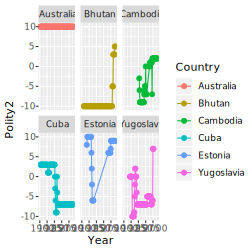
\includegraphics{insights_website_files/figure-latex/unnamed-chunk-28-1} \end{center}

\emph{Insight} That the polity score of a country can change so greatly has implications for our subsequent analyses. For example, calculating and using a mean polity score for each country (average across years) may be unwise as it would ignore such temporal change.

\hypertarget{acquire-import-check-the-fao-food-balance-sheet-data}{%
\section{Acquire, import, check the FAO Food balance sheet data}\label{acquire-import-check-the-fao-food-balance-sheet-data}}

This data shows, for various \emph{Areas} in the world, such as countries and continents, the annual supply and use of various food \emph{Items} such as ``Wheat and products'', ``Honey'', and ``Crustaceans''. Supply and use includes what are called \emph{Elements} of the food supply equation; elements such as ``Production'', Import Quantity``, and''Food supply quantity (kg/capita/yr)". The words \emph{Area}, \emph{Item}, and \emph{Element} are emphasised because they are variables in the dataset, as described further below. There is a lot of important information about this data available on the \href{http://www.fao.org/faostat/en/\#data/FBS/metadata}{FAO Food Balance Sheet Metadata} web page web page. And even more in the \href{http://www.fao.org/economic/ess/fbs/ess-fbs02/en/}{Food Balance Sheet Methodology Handbook}.

The full dataset is about 210MB and can be downloaded from the FAO web page. Importing this takes about 4 seconds on a reasonably fast laptop. As you will see below, we will make a smaller dataset (about 15MB) and save it, so we don't have to work with the full dataset.

The full dataset has 238,560 rows and 113 variables. The first nine variables are:

\begin{itemize}
\tightlist
\item
  \textbf{Area.code} - A numeric variable containing number codes for the \emph{Area} variable.
\item
  \textbf{Area} - A character variable containing the geographic area that a row is about, for example, a country name or a continent name.
\item
  \textbf{Item.code} - A numeric variable containing number codes for the food items in the \emph{Item} variable.
\item
  \textbf{Item} - A character variable containing the food item a row is about.
\item
  \textbf{Element.code} - A numeric variable contains number codes for the \emph{Element} variable.
\item
  \textbf{Element} - A character variable showing the particular supply or utlilisation element a row is about. These are the elements of the food balance equation.
\item
  \textbf{Unit} - The units of measure of the quantity in the row.
\item
  \textbf{Y1961} - A numeric variable giving the quantity in year 1961
\item
  \textbf{Y1961F} - A character variable giving information about the data (F is for Flag), such as ``Official data'', ``FAO data'', etc.
\end{itemize}

The \emph{Definitions and standard button} on this web page \url{http://www.fao.org/faostat/en/\#data/FBS/metadata} leads to much much more information about the variables and entries.

You could get the FAO food balance data from the \href{http://www.fao.org/faostat/en/\#data/FBS/metadata}{FAO website}. The datafile you would get is called \texttt{FoodBalanceSheets\_E\_All\_Data.csv} and is 206MB, i.e.~it is quite big. We need, however, only a small amount of the information in this dataset. So to make things easier for ourselves and for you, we created a smaller dataset containing only the data we need, and saved it as an \texttt{Rdata} file. This file type fits more data into a smaller space---the resulting file \texttt{FoodBalanceSheets\_E\_All\_Data\_reduced.Rdata} is 1.9MB. We put this smaller data file on the \href{insightsfromdata.io}{Insights Website}, so if you don't want to make it yourself, please get it from there.

If you do want to go through this process, feel free to use the code immediately below, otherwise skip over this. It's pretty straightforward, apart from two things. First, we give the \texttt{read\_csv} an argument you didn't previously see: \texttt{encoding}. This helps \texttt{read\_csv} properly recognise otherwise problematic symbols. In this case, it ensure that country names such as \emph{Côte d'Ivoire} don't cause problems (the ô can do so). Second, the penultimate line saves the produced tibble \texttt{ff} to a \texttt{Rdata} type of data file; though even that new type of instruction should be quite transparent to you by now.

\begin{Shaded}
\begin{Highlighting}[]
\CommentTok{## Get the full food balance sheet dataset *All data* from the FAO website:}
\CommentTok{## http://www.fao.org/faostat/en/#data/FBS/metadata.}
\CommentTok{## Reduce the size of the FAO data, so easier to deal with}
\CommentTok{## import FAO data}
\NormalTok{ff <-}\StringTok{ }\KeywordTok{read_csv}\NormalTok{(}\StringTok{"data/FoodBalanceSheets_E_All_Data.csv"}\NormalTok{,}
               \DataTypeTok{locale =} \KeywordTok{locale}\NormalTok{(}\DataTypeTok{encoding =} \StringTok{'ISO-8859-1'}\NormalTok{))}
\CommentTok{## First fix some variable names:}
\KeywordTok{names}\NormalTok{(ff) <-}\StringTok{ }\KeywordTok{str_replace_all}\NormalTok{(}\KeywordTok{names}\NormalTok{(ff), }\KeywordTok{c}\NormalTok{(}\StringTok{" "}\NormalTok{ =}\StringTok{ "_"}\NormalTok{))}
\CommentTok{## Remove all non-countries}
\NormalTok{ff <-}\StringTok{ }\KeywordTok{filter}\NormalTok{(ff, Country_Code }\OperatorTok{<}\StringTok{ }\DecValTok{5000}\NormalTok{)}
\CommentTok{## keep only some of the elements}
\NormalTok{ff <-}\StringTok{ }\KeywordTok{filter}\NormalTok{(ff, Element }\OperatorTok\StringTok{ }\KeywordTok{c}\NormalTok{(}\StringTok{"Food supply quantity (kg/capita/yr)"}\NormalTok{))}
\CommentTok{## remove some other variables that won't be used}
\NormalTok{ff <-}\StringTok{ }\KeywordTok{select}\NormalTok{(ff, }\OperatorTok{-}\NormalTok{Country_Code, }\OperatorTok{-}\NormalTok{Item_Code,}
             \OperatorTok{-}\NormalTok{Element_Code, }\OperatorTok{-}\NormalTok{Element, }\OperatorTok{-}\NormalTok{Unit,}
             \OperatorTok{-}\KeywordTok{ends_with}\NormalTok{(}\StringTok{"F"}\NormalTok{))}
\CommentTok{## save the reduced file}
\KeywordTok{saveRDS}\NormalTok{(ff, }\StringTok{"data/FoodBalanceSheets_E_All_Data_reduced.Rdata"}\NormalTok{)}
\KeywordTok{rm}\NormalTok{(ff)}
\end{Highlighting}
\end{Shaded}

The next line reads in that smaller dataset:

\begin{Shaded}
\begin{Highlighting}[]
\CommentTok{#rm(list = ls())}
\NormalTok{fbs <-}\StringTok{ }\KeywordTok{readRDS}\NormalTok{(}\StringTok{"data/FoodBalanceSheets_E_All_Data_reduced.Rdata"}\NormalTok{)}
\end{Highlighting}
\end{Shaded}

Feel free to have a look at the whole dataset with the \texttt{skim} function. We \texttt{select} a few columns first, as otherwise the output is rather long due to there being 112 variables in the dataset.

\begin{Shaded}
\begin{Highlighting}[]
\CommentTok{#select(fbs, Country, Item, Y1961, Y1971, Y1981, Y1991, Y2001, Y2011) %>%}
\CommentTok{#  skim()}
\end{Highlighting}
\end{Shaded}

There are 17'953 observations/rows in the tibble. There are 182 countries, so 11 fewer than in the Polity data. We will later check which ones are not in the Polity data, and if any in the Polity data are not in the FAO data. There are 114 food \texttt{Items}\ldots{} wow, that's a lot of different types of food! Take a look at some of the values\ldots{} it's quite interesting to see what's recorded. Both the \texttt{Country} variable and the \texttt{Item} variable are characters type variables as expected. If the data contained every possible combination of country and item we would expect 182 * 114 = 20'748 observations. That there are only 17'953 tells us that some combinations are missing. We will find out which these are.

The six year variables are, as expected numeric---they are amounts of food available (food supply quantities in kg per capita per year). We see there are quite a lot of missing values in the earlier years, and fewer in the later years. This might be expected if development of methods and adoption of them becomes more complete through time.

\hypertarget{tidying-FAO}{%
\subsection{Tidy the FAO data}\label{tidying-FAO}}

The FAO data is not tidy. You should be able to figure out in what respect it is ``dirty''. Yes, the same information is spread across multiple columns/variables, such that there are multiple observations in each row. More specifically, the data for each year is in a separate column---data for different years are spread across columns---each row contains lots of observations each from a different year.

Before we make the data tidy, let's try to figure out how many rows it should have when tidy. We will gather all the information that is currently spread across columns and put it in one column. A visualisation of a simplified version of the dataset is in Figure \ref{fig:long-wide}. The answer is the amount of information that's in the columns that we want to gather into a single column. In the untidy/wide data there are 55 variables containing the data we wish to gather (because we are not gathering the information from \texttt{Country} or \texttt{Item}). Each of those variables has 17,953 rows, so we expect the long/tidy data to have 55 * 17,953 = 987,415 rows.

\begin{figure}

{\centering \includegraphics[width=1\linewidth]{images/long_wide} 

}

\caption{The same data (a) in long/tidy format and (b) in wide format, with colours and arrows linking the same data in the two different formats.}\label{fig:long-wide}
\end{figure}

Let's now make the data tidy, and clean up the year variable. We first gather all the same data from columns three through 57 (\texttt{3:57}) into a new variable called \texttt{Food\_Supply\_Quantity} and put the information about which year each observation belongs to in a new variable called \texttt{Year}. Because the column names begin with Y (e.g. \texttt{Y1961}) we then need to keep only the 2nd through to 5th character in the \texttt{Year} variable (using the \texttt{substr} function), and convert the result to a numeric type variable (with the \texttt{as.numeric} function), doing all this within a \texttt{mutate} in order to replace the old year variable with the converted one. Let's then take a look at the data with \texttt{skim}. Here's the code for all that:

\begin{Shaded}
\begin{Highlighting}[]
\NormalTok{fbs_long <-}\StringTok{ }\NormalTok{fbs }\OperatorTok
\StringTok{  }\KeywordTok{gather}\NormalTok{(}\DataTypeTok{key =}\NormalTok{ Year, }\DataTypeTok{value =}\NormalTok{ Food_Supply_Quantity, }\DecValTok{3}\OperatorTok{:}\DecValTok{57}\NormalTok{) }\OperatorTok
\StringTok{  }\KeywordTok{mutate}\NormalTok{(}\DataTypeTok{Year =} \KeywordTok{as.numeric}\NormalTok{(}\KeywordTok{substr}\NormalTok{(Year, }\DecValTok{2}\NormalTok{, }\DecValTok{5}\NormalTok{)))}
\CommentTok{#skim(fbs_long)}
\end{Highlighting}
\end{Shaded}

We see that as expected the new tibble contains 987,415. Excellent! This near-magical gather function has done a lot of very tedious work for us, very quickly. There are still the same number of countries (182) and food items (114). Now we see that the data covers from year 1961 to 2015. We also get the distribution of the food supply quantity variable\ldots{} it looks to have lots of small values, and a few large. Is this what you would expect? Perhaps supply is large for a few basic foods (e.g.~grains) and then there are lots of relatively rare food items. But beware that at present we are looking at the distribution including data from across years and countries. We will soon look more closely at this distribution. The \texttt{skim} also tells us that only the food supply quantity variable contains any missing values, and that there are 158,307 of them.

\hypertarget{clean-the-fao-data}{%
\subsection{Clean the FAO data}\label{clean-the-fao-data}}

Are all the years represented in the dataset? Let's look at the unique values of the year variable:

\begin{Shaded}
\begin{Highlighting}[]
\KeywordTok{unique}\NormalTok{(}\KeywordTok{pull}\NormalTok{(fbs_long, Year))}
\end{Highlighting}
\end{Shaded}

\begin{verbatim}
##  [1] 1961 1962 1963 1964 1965 1966 1967 1968 1969 1970 1971 1972 1973 1974
## [15] 1975 1976 1977 1978 1979 1980 1981 1982 1983 1984 1985 1986 1987 1988
## [29] 1989 1990 1991 1992 1993 1994 1995 1996 1997 1998 1999 2000 2001 2002
## [43] 2003 2004 2005 2006 2007 2008 2009 2010 2011 2012 2013 2014 2015
\end{verbatim}

Yes, every year from 1961 to 2015 is represented (by at least one observation). There are 15 years in the dataset.

Another good check to do on a dataset is for duplicated rows, if one can reasonably conclude that there should be none. Do we think there can be any duplicated rows in this dataset? That would be the exactly the same value of Country, Item, Year, and Food Supply Quantity.

Finding any duplicated rows is fairly straightforward thanks to the \texttt{duplicated} function, which returns a TRUE or FALSE for each row of a dataset, TRUE if the row is duplicated somewhere, or FALSE otherwise. Then we can \texttt{filter} the rows by these TRUE/FALSE values to give only the duplicated rows:

\begin{Shaded}
\begin{Highlighting}[]
\NormalTok{duplicated_records <-}\StringTok{ }\KeywordTok{filter}\NormalTok{(fbs_long, }\KeywordTok{duplicated}\NormalTok{(fbs_long))}
\end{Highlighting}
\end{Shaded}

Note that the resulting tibble contains only one example of each duplicate (look at the data with \texttt{View(duplicated\_rows)}.

There are, in fact, 9,287 rows that are duplicated (not unique). Let's assume that these are mistaken duplicate entries, and so reduce to a dataset with only unique rows:

\begin{Shaded}
\begin{Highlighting}[]
\NormalTok{fbs_long <-}\StringTok{ }\KeywordTok{unique}\NormalTok{(fbs_long)}
\end{Highlighting}
\end{Shaded}

Now, if we're being really paranoid, we might wonder if there were ever two different values of food supply recorded for the same country in the same year. Put another way, if we look at only the Country, Year, and Item variables, do we see duplicated rows?

\begin{Shaded}
\begin{Highlighting}[]
\NormalTok{part_duplicated_records <-}\StringTok{ }\NormalTok{fbs_long }\OperatorTok
\StringTok{  }\KeywordTok{select}\NormalTok{(Country, Item, Year) }\OperatorTok
\StringTok{  }\KeywordTok{duplicated}\NormalTok{() }\OperatorTok
\StringTok{  }\KeywordTok{filter}\NormalTok{(fbs_long, .)}
\end{Highlighting}
\end{Shaded}

Looking at the result we see there are 10,733 rows with duplicated Country, Year, and Item. This is weird. And that these duplicates are only for food items ``Eggs'' and ``Milk - Excluding Butter''. We have no idea why there are multiple entries for these two items! Here's an example of one of the duplicates:

\begin{Shaded}
\begin{Highlighting}[]
\KeywordTok{filter}\NormalTok{(fbs_long,}
\NormalTok{       Country }\OperatorTok{==}\StringTok{ "Albania"}\NormalTok{,}
\NormalTok{       Item }\OperatorTok{==}\StringTok{ "Eggs"}\NormalTok{,}
\NormalTok{       Year }\OperatorTok{==}\StringTok{ }\DecValTok{1961}\NormalTok{)}
\end{Highlighting}
\end{Shaded}

\begin{verbatim}
## # A tibble: 2 x 4
##   Country Item   Year Food_Supply_Quantity
##   <chr>   <chr> <dbl>                <dbl>
## 1 Albania Eggs   1961                  1.5
## 2 Albania Eggs   1961                  1.8
\end{verbatim}

In the same year for the same country there are two values of Food\_Supply\_Quantity: 1.5 and 1.8. But it's quite reasonable to think there can be only one. Let's solve this problem by rather arbitrarily calculating one value, the average, of these duplicated records:

\begin{Shaded}
\begin{Highlighting}[]
\NormalTok{fbs_long <-}\StringTok{ }\NormalTok{fbs_long }\OperatorTok
\StringTok{  }\KeywordTok{group_by}\NormalTok{(Country, Year, Item) }\OperatorTok
\StringTok{  }\KeywordTok{summarise}\NormalTok{(}\DataTypeTok{Food_Supply_Quantity =} \KeywordTok{mean}\NormalTok{(Food_Supply_Quantity)) }\OperatorTok
\StringTok{  }\KeywordTok{ungroup}\NormalTok{(fbs_long)}
\end{Highlighting}
\end{Shaded}

\begin{info}
Time to tell the truth. It took us a long long time to realise there
were duplicated records in the FAO dataset. We did not pro-actively
think to check for duplicates. We only realised there must be duplicates
when we tried to get the numbers to add up below. They did not before we
removed the duplicates, and this led us to find the duplicates. Once we
found them, we removed them above. Now it looks like we were really
smart to think they might occur, check for them, find them, and remove
them. In reality we were not so smart. What we were, however, was
**absolutely determined* to understand why the numbers did not add up.
You must also be as strict in your work. After we found the duplicates
in this dataset, we also looked in the Polity data, found some, and then
decided to add a check for duplicates to all case studies, and to advise
you to make this a standard sanity check when you start looking at a
dataset.
\end{info}

That was a major step forward. Now we know our dataset has only unique observations.

Now let's do another sanity check. Because there are 182 countries and 114 food items we know there could be 20,748 observations for each year. Let's see how many there really are:

\begin{Shaded}
\begin{Highlighting}[]
\NormalTok{obs_per_year <-}\StringTok{ }\NormalTok{fbs_long }\OperatorTok
\StringTok{  }\KeywordTok{group_by}\NormalTok{(Year) }\OperatorTok
\StringTok{  }\KeywordTok{summarise}\NormalTok{(}\DataTypeTok{num =} \KeywordTok{n}\NormalTok{())}
\end{Highlighting}
\end{Shaded}

There are only 17,589 observation per year. Either not all countries reported in all years, not all items were reported by each country in each year, or both!

First let's see how many countries there are per year:

\begin{Shaded}
\begin{Highlighting}[]
\NormalTok{countries_per_year <-}\StringTok{ }\NormalTok{fbs_long }\OperatorTok
\StringTok{  }\KeywordTok{group_by}\NormalTok{(Year) }\OperatorTok
\StringTok{  }\KeywordTok{summarise}\NormalTok{(}\DataTypeTok{num =} \KeywordTok{length}\NormalTok{(}\KeywordTok{unique}\NormalTok{(Country)))}
\end{Highlighting}
\end{Shaded}

There are indeed 182 countries per year. All countries are included in all years.

Let's see how many Items each country reported (across all years):

\begin{Shaded}
\begin{Highlighting}[]
\NormalTok{items_per_country <-}\StringTok{ }\NormalTok{fbs_long }\OperatorTok
\StringTok{  }\KeywordTok{group_by}\NormalTok{(Country) }\OperatorTok
\StringTok{  }\KeywordTok{summarise}\NormalTok{(}\DataTypeTok{num =} \KeywordTok{length}\NormalTok{(}\KeywordTok{unique}\NormalTok{(Item)))}
\end{Highlighting}
\end{Shaded}

Aha. Not all items were reported by all countries. Turkmenistan reported on the fewest (62), while China reported on the most (110). Let's see if the sum of the number of items reported by each country is the number of observations per year.

\begin{Shaded}
\begin{Highlighting}[]
\KeywordTok{sum}\NormalTok{(}\KeywordTok{pull}\NormalTok{(items_per_country, num))}
\end{Highlighting}
\end{Shaded}

\begin{verbatim}
## [1] 17589
\end{verbatim}

Yes! This is the same as the number of observations per year. All this pretty much guarantees that each country consistently (across all years) reported on a constant set of the items, or there is an observation for this set of items in each year.

\begin{safety}
We didn't just now find out anything new about the data, but we did
confirm that we understand it properly. Checks and balances increase
confidence.
\end{safety}

Now let's look at the missing values:

\begin{Shaded}
\begin{Highlighting}[]
\CommentTok{#skim(fbs_long)}
\end{Highlighting}
\end{Shaded}

We still have 155,003 missing values. Why? Where are they coming from?

Let's dig a bit deeper by getting the number of observations per year, and the number and proportion of these that are missing values:

\begin{Shaded}
\begin{Highlighting}[]
\NormalTok{obs_per_year <-}\StringTok{ }\NormalTok{fbs_long }\OperatorTok
\StringTok{  }\KeywordTok{group_by}\NormalTok{(Year) }\OperatorTok
\StringTok{  }\KeywordTok{summarise}\NormalTok{(}\DataTypeTok{num =} \KeywordTok{n}\NormalTok{(),}
            \DataTypeTok{num_na =} \KeywordTok{sum}\NormalTok{(}\KeywordTok{is.na}\NormalTok{(Food_Supply_Quantity)),}
            \DataTypeTok{prop_na =}\NormalTok{ num_na }\OperatorTok{/}\StringTok{ }\NormalTok{num)}
\end{Highlighting}
\end{Shaded}

And take a look at the data using \texttt{View(obs\_per\_year)}. We can also see quite a bit if we plot the summary data (\ref{fig:long-wide}) with the following code:

\begin{figure}

{\centering 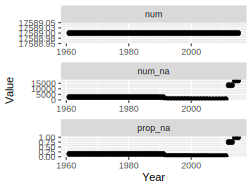
\includegraphics[width=1\linewidth]{insights_website_files/figure-latex/fao-pol1-1} 

}

\caption{The number of observations, the number of missing values and the proportion of missing values in each year of the data.}\label{fig:fao-pol1}
\end{figure}

We see that from 1961 to 1989 there are 2,592 (14.74\%) missing values per year. In 1990 and 1991 there are 2,493 (14.17\%) missing values per year. From 1992 to 2011 less than 5\% of the values are missing, and from 2012 to 2015 (the last year in the dataset) most or all the values are missing. Can you think of why there might be fewer missing values after 1991? Let's look at one country (its identity might give you a clue)\ldots{} Belarus. Let's get the number of values, missing values, and proportion of missing values for Belarus in each year.

\begin{Shaded}
\begin{Highlighting}[]
\NormalTok{Belarus_obs_per_year <-}\StringTok{ }\NormalTok{fbs_long }\OperatorTok
\StringTok{  }\KeywordTok{filter}\NormalTok{(Country }\OperatorTok{==}\StringTok{ "Belarus"}\NormalTok{) }\OperatorTok
\StringTok{  }\KeywordTok{group_by}\NormalTok{(Year) }\OperatorTok
\StringTok{  }\KeywordTok{summarise}\NormalTok{(}\DataTypeTok{num =} \KeywordTok{n}\NormalTok{(),}
            \DataTypeTok{num_na =} \KeywordTok{sum}\NormalTok{(}\KeywordTok{is.na}\NormalTok{(Food_Supply_Quantity)),}
            \DataTypeTok{prop_na =}\NormalTok{ num_na }\OperatorTok{/}\StringTok{ }\NormalTok{num)}
\end{Highlighting}
\end{Shaded}

Looking at this dataset we see that all values are missing until 1992, and then there are no missing values until 2012, when all are again missing. it's probably clear by now that all values are missing until 1992 because Belarus only became an independent state in 1991. Likely there are lots of other countries in the dataset that have missing values for this reason.

There's some other weird stuff going on here: Belgium and Luxembourg did not separately report data during the period 1992-1999, and instead reported jointly. Then from 2000 until 2011 reported separately, so there we have lots of missing values. Then we have some countries that ceased to exist in their former state, e.g.~Czechoslovakia after 1993 contains only missing values due to its dissolution into the Czech Republic and Slovakia. Similarly, USSR reports only missing values after 1991 when the USSR collapsed.

And why more missing values from 2012 to 2015? Actually, the description of the data on the FAO web site says the data is from 1961 to only 2013, so it's not surprising that 2014 and 2015 are empty. We will remove these years. We don't know why there are more missing values in 2012 and 2013, so let's also remove those:

\begin{Shaded}
\begin{Highlighting}[]
\NormalTok{fbs_long <-}\StringTok{ }\KeywordTok{filter}\NormalTok{(fbs_long, Year }\OperatorTok{<}\StringTok{ }\DecValTok{2012}\NormalTok{)}
\CommentTok{#skim(fbs_long)}
\end{Highlighting}
\end{Shaded}

\textbf{What are we going to do???} This seems very messy! Let's aim for a dataset that contains only country/year combinations where a country actually existed (i.e.~there were not all NAs reported), and also where there is an entry for all 114 food items for each country year combination (by putting zeros in for no reported item).

First we get a list of years in which each country does not contain all missing values. This we will use as a master list of years and countries to include in our analysis. We will not include year/country combinations where there were only missing values (the reason we need to be this specific is that we will soon turn the missing values into zeros). Let's get that list of country/year combinations to include:

\begin{Shaded}
\begin{Highlighting}[]
\NormalTok{country_year_not_all_missing <-}\StringTok{ }\NormalTok{fbs_long }\OperatorTok
\StringTok{  }\KeywordTok{group_by}\NormalTok{(Country, Year) }\OperatorTok
\StringTok{  }\KeywordTok{summarise}\NormalTok{(}\DataTypeTok{keep =} \KeywordTok{n}\NormalTok{() }\OperatorTok{!=}\StringTok{ }\KeywordTok{sum}\NormalTok{(}\KeywordTok{is.na}\NormalTok{(Food_Supply_Quantity))) }\OperatorTok
\StringTok{  }\KeywordTok{filter}\NormalTok{(keep) }\OperatorTok
\StringTok{  }\KeywordTok{select}\NormalTok{(}\OperatorTok{-}\NormalTok{keep) }\OperatorTok
\StringTok{  }\KeywordTok{ungroup}\NormalTok{()}
\end{Highlighting}
\end{Shaded}

Does that look rather complicated? The difficult(ish) line is the summarise, in which we create a new variable \texttt{keep} that is TRUE or FALSE depending if all values of \texttt{Food\_Supply\_Quantity} are NA or not. The \texttt{n()} give the number of values, the \texttt{sum(is.na(Food\_Supply\_Quantity))} gives the number of NAs, and the \texttt{!=} asks if the two are not the same, and returns TRUE if so. The other lines should be possible for you to work out (though not necessarily easy).

Note that there are 8,272 combinations of years and countries in the dataset. This is an important number. It is the number of data points we should have data for after we calculate the diversity of food available in each country in each year.

Now we must decide what to assume when a country did not report a value for an item. We will assume that this means there was always zero supply of that food item, so the country did not bother ever including it, i.e.~it's really a zero. Hence we're going to pad out the data so that all countries report on all 114 items, with zero \texttt{Food\ Supply\ Quantity} for the items they did not report.

First we make a dataset the all combinations of \texttt{Country}, \texttt{Year}, and \texttt{Item}. It should have 182 * 51 * 182 = 1,058,148 rows. We use the quite lovely \texttt{expand.grid} function, which creates all possible combinations of the variables it's given. We give it all the unique values of \texttt{Country}, \texttt{Year}, and \texttt{Item}, and it expands them to give all possible combinations. Each argument to \texttt{expand.grid} should be a name-value pair, and the name should be the same in the original data, to aid further operations:

\begin{Shaded}
\begin{Highlighting}[]
\NormalTok{all_cases <-}\StringTok{ }\KeywordTok{expand.grid}\NormalTok{(}\DataTypeTok{Country =} \KeywordTok{unique}\NormalTok{(}\KeywordTok{pull}\NormalTok{(fbs_long, Country)),}
                         \DataTypeTok{Year =} \KeywordTok{unique}\NormalTok{(}\KeywordTok{pull}\NormalTok{(fbs_long, Year)),}
                         \DataTypeTok{Item =} \KeywordTok{unique}\NormalTok{(}\KeywordTok{pull}\NormalTok{(fbs_long, Item))) }
\end{Highlighting}
\end{Shaded}

Super. This has 1,058,148 rows as expected. Now we want to only keep from this the country/year combinations for which we already found there were countries that existed. There are 8,272 of these and each should have 114 items, so we should get 943,008 observations. We do this with a \texttt{left\_join} to keep only the cases of the join that have values in the first (left) dataset in the join:

\begin{Shaded}
\begin{Highlighting}[]
\NormalTok{temp2 <-}\StringTok{ }\KeywordTok{left_join}\NormalTok{(country_year_not_all_missing, all_cases)}
\end{Highlighting}
\end{Shaded}

\begin{verbatim}
## Joining, by = c("Country", "Year")
\end{verbatim}

\begin{verbatim}
## Warning: Column `Country` joining character vector and factor, coercing
## into character vector
\end{verbatim}

We get a warning, and know that we should never ignore warnings. The warning is \emph{Column \texttt{Country} joining character vector and factor, coercing into character vector}. This is caused because \texttt{expand.grid} automatically converts character variables to factors. We can stop this happening (by adding the argument \texttt{stringsAsFactors\ =\ FALSE} in our call to \texttt{expand.grid} and hopefully the remove the warning:

\begin{Shaded}
\begin{Highlighting}[]
\NormalTok{all_cases <-}\StringTok{ }\KeywordTok{expand.grid}\NormalTok{(}\DataTypeTok{Country =} \KeywordTok{unique}\NormalTok{(}\KeywordTok{pull}\NormalTok{(fbs_long, Country)),}
                         \DataTypeTok{Year =} \KeywordTok{unique}\NormalTok{(}\KeywordTok{pull}\NormalTok{(fbs_long, Year)),}
                         \DataTypeTok{Item =} \KeywordTok{unique}\NormalTok{(}\KeywordTok{pull}\NormalTok{(fbs_long, Item)),}
                         \DataTypeTok{stringsAsFactors =} \OtherTok{FALSE}\NormalTok{)}
\NormalTok{temp2 <-}\StringTok{ }\KeywordTok{left_join}\NormalTok{(country_year_not_all_missing, all_cases)}
\end{Highlighting}
\end{Shaded}

\begin{verbatim}
## Joining, by = c("Country", "Year")
\end{verbatim}

Perfect\ldots{} and we have the expected number of 943,008 observations.

Next we do another left join to add the food supply quantity data (in \texttt{fbs\_long}) to the cases/observations we want to keep (in \texttt{temp2})

\begin{Shaded}
\begin{Highlighting}[]
\NormalTok{temp3 <-}\StringTok{ }\KeywordTok{left_join}\NormalTok{(temp2, fbs_long)}
\end{Highlighting}
\end{Shaded}

\begin{verbatim}
## Joining, by = c("Country", "Year", "Item")
\end{verbatim}

Good, we still have 943'008 observations.

\begin{Shaded}
\begin{Highlighting}[]
\CommentTok{#skim(temp3)}
\end{Highlighting}
\end{Shaded}

The number of missing values is now 139,252. Each of these is a case when a country reported values for some items in a year, but did not report values for others, and these others are given a value of NA. As we said above, we're going to assume these are real zeros, and so we need to turn them all into zeros:

\begin{Shaded}
\begin{Highlighting}[]
\NormalTok{fao_final <-}\StringTok{ }\NormalTok{temp3 }\OperatorTok
\StringTok{  }\KeywordTok{mutate}\NormalTok{(}\DataTypeTok{Food_Supply_Quantity =} \KeywordTok{ifelse}\NormalTok{(}\OperatorTok{!}\KeywordTok{is.na}\NormalTok{(Food_Supply_Quantity),}
\NormalTok{                                       Food_Supply_Quantity,}
                                       \DecValTok{0}\NormalTok{))}
\CommentTok{#skim(fao_final)}
\end{Highlighting}
\end{Shaded}

No missing values now. And we have a dataset that we very well understand. Let's check again though.

We should have 114 items reported per country per year:

\begin{Shaded}
\begin{Highlighting}[]
\NormalTok{items_per_country_per_year <-}\StringTok{ }\NormalTok{fao_final }\OperatorTok
\StringTok{  }\KeywordTok{group_by}\NormalTok{(Country, Year) }\OperatorTok
\StringTok{  }\KeywordTok{summarise}\NormalTok{(}\DataTypeTok{num =} \KeywordTok{length}\NormalTok{(}\KeywordTok{unique}\NormalTok{(Item)))}
\end{Highlighting}
\end{Shaded}

And we should have varying numbers of countries per year:

\begin{Shaded}
\begin{Highlighting}[]
\NormalTok{countries_per_year <-}\StringTok{ }\NormalTok{fao_final }\OperatorTok
\StringTok{  }\KeywordTok{group_by}\NormalTok{(Year) }\OperatorTok
\StringTok{  }\KeywordTok{summarise}\NormalTok{(}\DataTypeTok{num =} \KeywordTok{length}\NormalTok{(}\KeywordTok{unique}\NormalTok{(Country)))}
\end{Highlighting}
\end{Shaded}

And the sum of the number of countries per year multiplied by 114 should equal 943,008:

\begin{Shaded}
\begin{Highlighting}[]
\KeywordTok{sum}\NormalTok{(}\KeywordTok{pull}\NormalTok{(countries_per_year, num)) }\OperatorTok{*}\StringTok{ }\DecValTok{114}
\end{Highlighting}
\end{Shaded}

\begin{verbatim}
## [1] 943008
\end{verbatim}

Yes! Wow! Can you believe so much effort was needed to make a solid foundation of data! And we're not even there yet\ldots{} we still have wrangling work to do: we need to merge/join the FAO and the Polity datasets. But first\ldots{}

\hypertarget{calculating-our-response-variables}{%
\subsection{Calculating our response variables}\label{calculating-our-response-variables}}

The final step of preparation of the FAO data is to calculate our response variables. Our question is about food diversity so we need response variables that quantify this. We will use number of items available per year, and diversity of items available per year, where diversity accounts for the amount of each item as well as number of items using the Shannon index.

\begin{Shaded}
\begin{Highlighting}[]
\NormalTok{fao_div <-}\StringTok{ }\NormalTok{fao_final }\OperatorTok
\StringTok{  }\KeywordTok{group_by}\NormalTok{(Country, Year) }\OperatorTok
\StringTok{  }\KeywordTok{summarise}\NormalTok{(}\DataTypeTok{diversity =} \KeywordTok{diversity}\NormalTok{(Food_Supply_Quantity,}
                                        \DataTypeTok{index =} \StringTok{"shannon"}\NormalTok{),}
            \DataTypeTok{richness =} \KeywordTok{sum}\NormalTok{(Food_Supply_Quantity}\OperatorTok{>}\DecValTok{0}\NormalTok{)) }\OperatorTok
\StringTok{  }\KeywordTok{ungroup}\NormalTok{(fao_div)}
\end{Highlighting}
\end{Shaded}

Excellent. We have 8,272 data points, exactly as we should. (We previously saw this was the number of combinations of country and year for which not all data was NA. I.e. the number of rows in \texttt{country\_year\_not\_all\_missing}).

\hypertarget{merge-the-two-datasets}{%
\section{Merge the two datasets}\label{merge-the-two-datasets}}

The final step of data preparation is to merge the Polity and FAO data. One nasty issue we must deal with before we do the merge is to check the country names in the two datasets. It's quite possible, even likely, there are instances of the same country having different names in the two. The following code gets the country names from each, looks for ones that appear in one and not the other, and vice versa, and writes these to csv files.

\begin{Shaded}
\begin{Highlighting}[]
\NormalTok{pol_countries <-}\StringTok{ }\KeywordTok{unique}\NormalTok{(}\KeywordTok{pull}\NormalTok{(pol, Country))}
\NormalTok{fao_countries <-}\StringTok{ }\KeywordTok{unique}\NormalTok{(}\KeywordTok{pull}\NormalTok{(fao_div, Country))}
\NormalTok{in_pol <-}\StringTok{ }\KeywordTok{setdiff}\NormalTok{(pol_countries, fao_countries)}
\NormalTok{in_fao <-}\StringTok{ }\KeywordTok{setdiff}\NormalTok{(fao_countries, pol_countries)}
\KeywordTok{write_csv}\NormalTok{(}\KeywordTok{tibble}\NormalTok{(in_pol), }\StringTok{"data/in_pol.csv"}\NormalTok{)}
\KeywordTok{write_csv}\NormalTok{(}\KeywordTok{tibble}\NormalTok{(in_fao), }\StringTok{"data/in_fao.csv"}\NormalTok{)}
\end{Highlighting}
\end{Shaded}

Then it's a matter of some manual spreadsheet work to find the matches, and to put these in a data file, and bring that matching back into R. You can get the country matching data file \texttt{countryname\_map.csv} from \url{http://insightsfromdata.io}.

\begin{Shaded}
\begin{Highlighting}[]
\NormalTok{countryname_map <-}\StringTok{ }\KeywordTok{read_csv}\NormalTok{(}\StringTok{"data/countryname_map.csv"}\NormalTok{,}
                            \DataTypeTok{locale =} \KeywordTok{locale}\NormalTok{(}\DataTypeTok{encoding =} \StringTok{'ISO-8859-1'}\NormalTok{))}
\end{Highlighting}
\end{Shaded}

\begin{verbatim}
## Parsed with column specification:
## cols(
##   in_fao = col_character(),
##   in_pol = col_character()
## )
\end{verbatim}

Then we use a \texttt{left\_join} to match the Country names in the Polity data to the those in the mapping dataset, which in effect adds a variable to the polity data that is the name of the countries in the FAO data. We then replace the Country variable with one that contains the FAO names if they exist, otherwise the Polity name:

\begin{Shaded}
\begin{Highlighting}[]
\NormalTok{pol1 <-}\StringTok{ }\KeywordTok{left_join}\NormalTok{(pol, countryname_map, }\DataTypeTok{by =}\KeywordTok{c}\NormalTok{ (}\StringTok{"Country"}\NormalTok{ =}\StringTok{ "in_pol"}\NormalTok{)) }\OperatorTok
\StringTok{  }\KeywordTok{mutate}\NormalTok{(}\DataTypeTok{Country =} \KeywordTok{ifelse}\NormalTok{(}\KeywordTok{is.na}\NormalTok{(in_fao),}
\NormalTok{                                Country,}
\NormalTok{                                in_fao)) }\OperatorTok
\StringTok{  }\KeywordTok{select}\NormalTok{(}\OperatorTok{-}\NormalTok{in_fao)}
\CommentTok{#skim(pol1)}
\end{Highlighting}
\end{Shaded}

And let's check the effect of this renaming of countries on the number of NAs. Here is the merge of the FAO and Polity data on the original Polity country names:

\begin{Shaded}
\begin{Highlighting}[]
\NormalTok{fao_pol <-}\StringTok{ }\KeywordTok{left_join}\NormalTok{(fao_div, pol)}
\end{Highlighting}
\end{Shaded}

\begin{verbatim}
## Joining, by = c("Country", "Year")
\end{verbatim}

\begin{Shaded}
\begin{Highlighting}[]
\KeywordTok{sum}\NormalTok{(}\KeywordTok{is.na}\NormalTok{(}\KeywordTok{pull}\NormalTok{(fao_pol, Polity2)))}
\end{Highlighting}
\end{Shaded}

\begin{verbatim}
## [1] 2607
\end{verbatim}

We get 2,607 missing polity values. And here after the renaming:

\begin{Shaded}
\begin{Highlighting}[]
\NormalTok{dd1 <-}\StringTok{ }\KeywordTok{left_join}\NormalTok{(fao_div, pol1)}
\end{Highlighting}
\end{Shaded}

\begin{verbatim}
## Joining, by = c("Country", "Year")
\end{verbatim}

\begin{Shaded}
\begin{Highlighting}[]
\KeywordTok{sum}\NormalTok{(}\KeywordTok{is.na}\NormalTok{(}\KeywordTok{pull}\NormalTok{(dd1, Polity2)))}
\end{Highlighting}
\end{Shaded}

\begin{verbatim}
## [1] 1819
\end{verbatim}

Now we have 1,819 missing polity values. Fewer, but still quite a lot. These are countries in the FAO data that we couldn't find in the Polity data. This is a bit unsatisfactory, but we'll go with what we have. By the way, some of these missing values are despite the country being in the Polity data, e.g.~there were no Polity records for Afghanistan from 1979 to 1988, but there were for other years.

One last thing: let's remove the NAs from the dataset:

\begin{Shaded}
\begin{Highlighting}[]
\NormalTok{fao_pol <-}\StringTok{ }\KeywordTok{na.omit}\NormalTok{(fao_pol)}
\end{Highlighting}
\end{Shaded}

\hypertarget{tidying-up}{%
\section{Tidying up}\label{tidying-up}}

We have a lot of objects in R's brain. We only need one: \texttt{fao\_pol}. We can remove all the other variables. We don't need to run all the code above every time we do an analysis. In this situation we can save the \texttt{fao\_pol} dataset, remove everything from R's brain using \texttt{rm(list\ =\ ls())} or by clicking the little broom icon in RStudio, and load it again:

\begin{Shaded}
\begin{Highlighting}[]
\KeywordTok{saveRDS}\NormalTok{(fao_pol, }\StringTok{"data/fao_pol.Rdata"}\NormalTok{)}
\end{Highlighting}
\end{Shaded}

\begin{Shaded}
\begin{Highlighting}[]
\KeywordTok{rm}\NormalTok{(}\DataTypeTok{list =} \KeywordTok{ls}\NormalTok{())}
\NormalTok{fao_pol <-}\StringTok{ }\KeywordTok{readRDS}\NormalTok{(}\StringTok{"data/fao_pol.Rdata"}\NormalTok{)}
\end{Highlighting}
\end{Shaded}

\hypertarget{shapes}{%
\section{Shapes}\label{shapes}}

As usual we look at the distribution of our variables. First the distribution of number of food items available in each country, across all countries and all years. The code for this you are quite familiar with by now, using \texttt{ggplot} and \texttt{geom\_histogram} (Figure \ref{fig:fao-pol2}:

\begin{Shaded}
\begin{Highlighting}[]
\KeywordTok{ggplot}\NormalTok{(fao_pol, }\KeywordTok{aes}\NormalTok{(}\DataTypeTok{x =}\NormalTok{ richness)) }\OperatorTok{+}
\StringTok{  }\KeywordTok{geom_histogram}\NormalTok{(}\DataTypeTok{bins =} \DecValTok{10}\NormalTok{)}
\end{Highlighting}
\end{Shaded}

\begin{figure}

{\centering 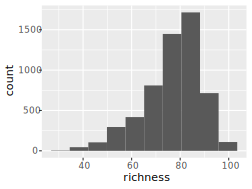
\includegraphics[width=0.75\linewidth]{insights_website_files/figure-latex/fao-pol2-1} 

}

\caption{Frequency distribution of richness of food items across all countries and years.}\label{fig:fao-pol2}
\end{figure}

Some countries in some years have only between 30 and 40 food items available, others have over 90. This is a large difference. The most common number is around 80. The distribution is somewhat left skewed, with a longer tail of smaller values. The distribution is not, however, horribly asymmetric.

And looking at the distribution of diversity of food item quantities with the following code (Figure \ref{fig:fao-pol3}:

\begin{Shaded}
\begin{Highlighting}[]
\KeywordTok{ggplot}\NormalTok{(fao_pol, }\KeywordTok{aes}\NormalTok{(}\DataTypeTok{x =}\NormalTok{ diversity)) }\OperatorTok{+}
\StringTok{  }\KeywordTok{geom_histogram}\NormalTok{(}\DataTypeTok{bins =} \DecValTok{10}\NormalTok{)}
\end{Highlighting}
\end{Shaded}

\begin{figure}

{\centering 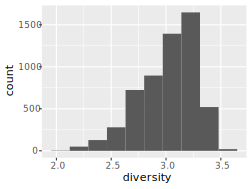
\includegraphics[width=0.75\linewidth]{insights_website_files/figure-latex/fao-pol3-1} 

}

\caption{Frequency distribution of diversity of food items across all countries and years.}\label{fig:fao-pol3}
\end{figure}

The diversity distribution is quite similar to the richness distribution, with a bit of left skew, but not too much. The values of diversity are rather arbitrary---not as intuitive as richness. Higher values indicate some combination of high richness and high evenness in the quantities of the items.

And looking at the distribution of the Polity variable with the following code (Figure \ref{fig:fao-pol3x}:

\begin{Shaded}
\begin{Highlighting}[]
\KeywordTok{ggplot}\NormalTok{(fao_pol, }\KeywordTok{aes}\NormalTok{(}\DataTypeTok{x =}\NormalTok{ Polity2)) }\OperatorTok{+}
\StringTok{  }\KeywordTok{geom_histogram}\NormalTok{(}\DataTypeTok{bins =} \DecValTok{10}\NormalTok{)}
\end{Highlighting}
\end{Shaded}

\begin{figure}

{\centering 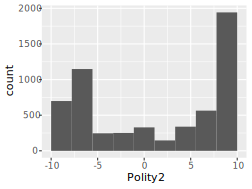
\includegraphics[width=0.75\linewidth]{insights_website_files/figure-latex/fao-pol3x-1} 

}

\caption{Frequency distribution of Polity2 all countries and years.}\label{fig:fao-pol3x}
\end{figure}

Is this what you were expecting? A rather bimodal distribution with most countries either very autocratic (low scores) or very democratic (high scores). Perhaps this in itself is an interesting pattern, though political scientists may find it obvious. Probably the creators of the Polity2 data have commented on it.

\hypertarget{relationships}{%
\section{Relationships}\label{relationships}}

First we'll look at the relationship between richness and diversity. We might imagine that they're quite closely associated since 1) diversity includes richness, and 2) their distributions look quite similar. By now the following code to make a scatter plot of richness against diversity should be familiar, though we add some transparency to the points since lots lie on top of each other (Figure \ref{fig:fao-pol4}:

\begin{Shaded}
\begin{Highlighting}[]
\KeywordTok{ggplot}\NormalTok{(fao_pol, }\KeywordTok{aes}\NormalTok{(}\DataTypeTok{x =}\NormalTok{ richness, }\DataTypeTok{y =}\NormalTok{ diversity)) }\OperatorTok{+}
\StringTok{  }\KeywordTok{geom_point}\NormalTok{(}\DataTypeTok{alpha =} \FloatTok{0.05}\NormalTok{)}
\end{Highlighting}
\end{Shaded}

\begin{figure}

{\centering \includegraphics[width=0.75\linewidth]{insights_website_files/figure-latex/fao-pol4-1} 

}

\caption{Relationship between the two response variables, richness of items and diversity of items, across all countries and years.}\label{fig:fao-pol4}
\end{figure}

Not quite as close a relationship as we expected. There is certainly enough spread that we could get different insights from looking at each of the variables separately\ldots{} they don't have to tell the same story.

And now, drum-roll, for the answer to our question. Is there a relationship between the political system of a country and the richness of food available for human consumption. Again, by now the R-code is hopefully no challenge for you (and gives Figure \ref{fig:fao-pol5}):

\begin{Shaded}
\begin{Highlighting}[]
\KeywordTok{ggplot}\NormalTok{(fao_pol, }\KeywordTok{aes}\NormalTok{(}\DataTypeTok{x =}\NormalTok{ Polity2, }\DataTypeTok{y =}\NormalTok{ richness)) }\OperatorTok{+}
\StringTok{  }\KeywordTok{geom_point}\NormalTok{(}\DataTypeTok{alpha =} \FloatTok{0.05}\NormalTok{)}
\end{Highlighting}
\end{Shaded}

\begin{figure}

{\centering 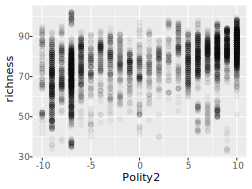
\includegraphics[width=0.75\linewidth]{insights_website_files/figure-latex/fao-pol5-1} 

}

\caption{Richness of food items available versus Polity score, across all countries and all available years.}\label{fig:fao-pol5}
\end{figure}

What do you think? Is there a relationship? And how confident are you that the relationship is not just the result of chance? Before we conclude, let's look at the relationship for diversity of food items (Figure \ref{fig:fao-pol6}).

\begin{Shaded}
\begin{Highlighting}[]
\KeywordTok{ggplot}\NormalTok{(fao_pol, }\KeywordTok{aes}\NormalTok{(}\DataTypeTok{x =}\NormalTok{ Polity2, }\DataTypeTok{y =}\NormalTok{ diversity)) }\OperatorTok{+}
\StringTok{  }\KeywordTok{geom_point}\NormalTok{(}\DataTypeTok{alpha =} \FloatTok{0.05}\NormalTok{)}
\end{Highlighting}
\end{Shaded}

\begin{figure}

{\centering 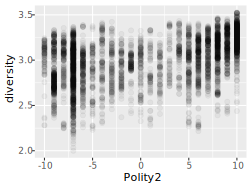
\includegraphics[width=0.75\linewidth]{insights_website_files/figure-latex/fao-pol6-1} 

}

\caption{Diversit of food items available versus Polity score, across all countries and all available years.}\label{fig:fao-pol6}
\end{figure}

Well, to our eyes, it certainly looks like the countries with high Polity scores have higher richness and diversity of food available than the countries with low Polity scores. There is also \emph{a lot} of variation, such that any country (regardless of Polity) can have nearly the highest or lowest observed diversity of richness.

We are being a little bit naughty, however. Each country can be contributing multiple data points to these graphs, one for each year it is present in the dataset. Countries with more years will tend to influence our conclusions more than those with fewer years. And the different years of data from one country are not independent\ldots{} they are repeated measures. Let's remove this non-independence and differential contributions of different countries in one of the crudest (though very simple and effective) ways---by getting the average value for each country. The \texttt{group\_by}, \texttt{summarise} we use should be familiar:

\begin{Shaded}
\begin{Highlighting}[]
\NormalTok{dd_year <-}\StringTok{ }\NormalTok{fao_pol }\OperatorTok
\StringTok{  }\KeywordTok{group_by}\NormalTok{(Country) }\OperatorTok
\StringTok{  }\KeywordTok{summarise}\NormalTok{(}\DataTypeTok{Polity2 =} \KeywordTok{mean}\NormalTok{(Polity2),}
            \DataTypeTok{richness =} \KeywordTok{mean}\NormalTok{(richness),}
            \DataTypeTok{diversity =} \KeywordTok{mean}\NormalTok{(diversity))}
\end{Highlighting}
\end{Shaded}

We have gone from a dataset with 5,665 observations to one with 133, one data point for each country in the data. Here's the code for the graphs of Polity score and richness/diversity for this country level data:

\begin{Shaded}
\begin{Highlighting}[]
\KeywordTok{ggplot}\NormalTok{(dd_year, }\KeywordTok{aes}\NormalTok{(}\DataTypeTok{x =}\NormalTok{ Polity2, }\DataTypeTok{y =}\NormalTok{ richness)) }\OperatorTok{+}
\StringTok{  }\KeywordTok{geom_point}\NormalTok{()}
\end{Highlighting}
\end{Shaded}

\begin{figure}

{\centering 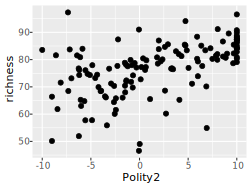
\includegraphics[width=0.75\linewidth]{insights_website_files/figure-latex/fao-pol7-1} 

}

\caption{Richness of food items available versus Polity score; average value for each country.}\label{fig:fao-pol7}
\end{figure}

\begin{Shaded}
\begin{Highlighting}[]
\KeywordTok{ggplot}\NormalTok{(dd_year, }\KeywordTok{aes}\NormalTok{(}\DataTypeTok{x =}\NormalTok{ Polity2, }\DataTypeTok{y =}\NormalTok{ diversity)) }\OperatorTok{+}
\StringTok{  }\KeywordTok{geom_point}\NormalTok{()}
\end{Highlighting}
\end{Shaded}

\begin{figure}

{\centering 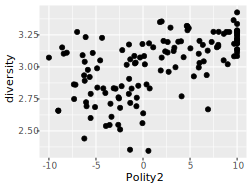
\includegraphics[width=0.75\linewidth]{insights_website_files/figure-latex/fao-pol8-1} 

}

\caption{Diversity of food items available versus Polity score; average value for each country.}\label{fig:fao-pol8}
\end{figure}

The country level data (Figures \ref{fig:fao-pol7} and \ref{fig:fao-pol8}) appear to show stronger evidence of a positive relationship between polity score and richness/diversity of food available, with more democratic countries (higher polity scores) having more diversity of food available than less democratic ones.

Let's look at the data another way, by categorising the Polity score. To do this we make a new variable using \texttt{mutate} and use the \texttt{cut} function to cut the Polity scores into five categories, and we name the categories:

\begin{Shaded}
\begin{Highlighting}[]
\NormalTok{dd_year <-}\StringTok{ }\NormalTok{dd_year }\OperatorTok
\StringTok{  }\KeywordTok{mutate}\NormalTok{(}\DataTypeTok{Polity2_cat =} \KeywordTok{cut}\NormalTok{(Polity2,}
                           \DataTypeTok{breaks =} \KeywordTok{seq}\NormalTok{(}\OperatorTok{-}\DecValTok{11}\NormalTok{, }\DecValTok{11}\NormalTok{, }\DataTypeTok{length =} \DecValTok{6}\NormalTok{),}
                           \DataTypeTok{labels =} \KeywordTok{c}\NormalTok{(}\StringTok{"Very autocratic"}\NormalTok{,}
                                      \StringTok{"Quite autocratic"}\NormalTok{,}
                                      \StringTok{"Neutral"}\NormalTok{,}
                                      \StringTok{"Quite democratic"}\NormalTok{,}
                                      \StringTok{"Very democratic"}\NormalTok{)))}
\end{Highlighting}
\end{Shaded}

Here, we will only show the figure for the richness of food items (Figures \ref{fig:fao-pol7}) and not diversity (you can make that graph yourself):

\begin{Shaded}
\begin{Highlighting}[]
\KeywordTok{ggplot}\NormalTok{(dd_year, }\KeywordTok{aes}\NormalTok{(}\DataTypeTok{x =}\NormalTok{ Polity2_cat, }\DataTypeTok{y =}\NormalTok{ richness)) }\OperatorTok{+}
\StringTok{  }\KeywordTok{geom_boxplot}\NormalTok{() }\OperatorTok{+}\StringTok{ }\KeywordTok{geom_beeswarm}\NormalTok{() }\OperatorTok{+}
\StringTok{  }\KeywordTok{ylab}\NormalTok{(}\StringTok{"Dietary richness}\CharTok{\textbackslash{}n}\StringTok{[number of food items]"}\NormalTok{) }\OperatorTok{+}
\StringTok{  }\KeywordTok{xlab}\NormalTok{(}\StringTok{"Type of political system"}\NormalTok{) }\OperatorTok{+}
\StringTok{  }\KeywordTok{coord_flip}\NormalTok{()}
\end{Highlighting}
\end{Shaded}

\begin{figure}

{\centering 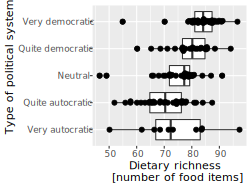
\includegraphics[width=0.75\linewidth]{insights_website_files/figure-latex/fao-pol9-1} 

}

\caption{Frequency distribution of diversity of food items across all countries and years.}\label{fig:fao-pol9}
\end{figure}

This tells more or less the same story, though the figure might be considered a bit nicer as it shows the meaning of the Polity score. There is an interest pattern we didn't note before, however: that the very autocratic countries seems to have somewhat higher food diversity than we might expect---quite similar to the countries with Neutral polities. There are relatively few of these very autocratic countries, however, and one of them (China) has the highest food richness of any country!

\hypertarget{wrapping-up}{%
\section{Wrapping up}\label{wrapping-up}}

Did you notice that we spent about 20 pages preparing the data, and then only ten or so (mostly graphs) looking at shapes and relationships? We spent much more time and effort making sure we knew the data inside out, that we had prepared it appropriately, and it was a solid foundation for the question we wanted to answer. And that most of the new practices and R code you experience were in that data preparation phase, and not in the analysis part.

That said, we were rather shallow in the analysis part. There is much much more we could have looked at. For example, we could look at relationships within countries across time, especially if there is a big shift in polity. Does the shift in polity precede a shift in diversity of food availability?

There are also lots of other explanatory variables we could have included in our analysis, for example national GDP, geographical location, and so on. Lots of this data is freely available on the internet. A simply fantastic place to get lost in such data and visualisation is the \href{https://ourworldindata.org/}{Our World in Data} website.

Other things you could think about analysing, for which data are available (though we couldn't say exactly where):

\begin{itemize}
\tightlist
\item
  Biodiversity
\item
  Latitudinal gradient
\item
  Species (country) area relationship
\item
  GDP diversity relationship.
\item
  Causality by time lag relationships.
\item
  FAO Macroeconomic statistics (e.g.~GDP by country by year) (\url{http://www.fao.org/faostat/en/\#data})
\item
  FAO Population data (e.g.~population size by country by year) (\url{http://www.fao.org/faostat/en/\#data})
\item
  World Bank, e.g.~country land area \url{https://data.worldbank.org/indicator/AG.LND.TOTL.K2}
\item
  Maybe: SDG indicators: \url{http://data.un.org/Explorer.aspx?d=SDGs}
\end{itemize}

\hypertarget{some-questions}{%
\section{Some questions}\label{some-questions}}

Go to the Insights companion website \url{http://insightsfromdata.io} and have a go at the questions and exercises for this chapter.

\hypertarget{WFD-3}{%
\chapter{Are more diverse diets better?}\label{WFD-3}}

\hypertarget{going-to-the-next-level}{%
\section{Going to the next level}\label{going-to-the-next-level}}

This case study includes a bit more complexity than the first one and covers a few new topics in R and in general. The complexity mainly occurs in the calculations we do to obtain the response variables (i.e.~the variables we examine to answer our biological question). The calculations involve some conceptually challenging manipulations, and the corresponding pipelines of \textbf{dplyr} functions will at first seem complex and daunting.

It's fine to be concerned, even a bit stressed, by this complexity. If you feel so, just take a break, have a chat with friends, and while doing that think about how we only travel great distances and climb high peaks by taking one small step at a time. The same applies to what seem like complex and daunting tasks in getting insights from data. It's amazing how far we get taking one step at a time. When we show you what seems like a complex task, like a complex pipeline of functions, break it down into its component steps. Let's take a first step by introducing the case study and data that was collected.

Again: as you work through this chapter, try following along with the \href{http://r4all.org/posts/workflow-checklist-for-data-analysis/}{workflow/checklist on this web page}.

\hypertarget{introduction-to-the-study-and-data-1}{%
\section{Introduction to the study and data}\label{introduction-to-the-study-and-data-1}}

The data comes from \href{https://besjournals.onlinelibrary.wiley.com/doi/abs/10.1046/j.1365-2656.2000.00446.x}{a study of how the number of available prey species for a predator consume affects the stability of the predator population dynamics}. The study was designed to address the hypotheses that more pathways of energy flow to a predator (i.e.~more prey species) would stabilise the predator population dynamics, 1) by increasing the abundance of the predator, 2) by reducing how much it varies, and 3) by delaying extinction.

The experiment involved three prey species and one predator. One, two or three prey species were present, with every combination of each. The experimental units were small jars of nutrient containing liquid and the predator and prey species were aquatic microbes feeding on bacteria also present in the liquid. The small size of the prey and predators (about 20 to 400 microns) means that in just a few weeks individuals can reproduce many times, and also die. There were five replicates of each of the seven prey species compositions (so 35 experimental units).

During the experiment the data was written onto paper, then at a later date the data was entered into a spreadsheet. The data in the spreadsheet was checked for errors, by comparing it with the original paper copy of the data. The data recording and entry was done with tidiness and cleanliness in mind, so tidying and cleaning will be minimal. The data file contains the data exactly as it was recorded on the paper data sheet, and after data entry was double checked to correct any errors.

Looking at the dataset in Excel or something similar, you will see the following variables:

\begin{itemize}
\tightlist
\item
  \textbf{day} - the day of the experiment the observation in the row belongs to.
\item
  \textbf{count} - the number of individuals counted in the sample; used to calculate density per ml. Counts were made by eye, looking down a microscope.
\item
  \textbf{w1} - the volume of liquid in ml removed from the community for sampling abundance. Used to calculate density per ml.
\item
  \textbf{w2} - the volume of diluent added to the volume sampled, plus the volume sampled. Used to calculate density per ml.
\item
  \textbf{w3} - the volume of the sub-sample taken of the mixture of diluent and sample removed. Used to calculate density per ml.
\item
  \textbf{species} - a numeric code for the species that the observation in the row belongs to.
\item
  \textbf{prey.richness} - the number of prey species added to the jar.
\item
  \textbf{prey.composition} - a number that identifies the combination of prey species added to the jar.
\item
  \textbf{replicate} - a replicate identifier, unique within prey composition.
\item
  \textbf{jar} - a number that uniquely identifies each experimental unit.
\end{itemize}

How does the data measure up to the features of data we mentioned in the first chapter?

\begin{itemize}
\tightlist
\item
  Number of variables. Not too many. Really there are only two or three explanatory variables, and one response variable (population size, though we will derive three separate response variables). Certainly we are not up in the range of tens of explanatory variables. And because this was an experiment, we only have variables already thought to be important.
\item
  Number of observations. Not too many. Just 35. Our ability to detect patterns is going to be low.
\item
  If and how many of the variables describe experimental manipulations. Yes the data are from an experiment. Prey composition was manipulated, and so therefore was prey richness. So we know that any apparent relationships between the predator population and the prey composition is a result of a causative relationships. I.e. if we alter prey composition and only prey composition (as is the case here) and see changes in the predator population then we know that prey composition \emph{caused} those changes.
\item
  The amount of correlation among the variables. There is no correlation to speak of; this is not so uncommon in an experiment.
\item
  How independent are the observations. Here we need to be a bit careful. There were 35 experimental units, so there should be 35 data points in our analyses. Multiple samples through time were taken from each experimental unit, however---we have repeated measures. We will take care of this, and not fall into a trap of trying to interpret patterns in graphs with lots of non-independent data points.
\end{itemize}

\hypertarget{what-type-of-response-variable}{%
\section{What type of response variable?}\label{what-type-of-response-variable}}

This question is worth asking at the beginning of a study. There were, in fact, three main response variables used in this study and these correspond to the three hypotheses mentioned above. I.e. there is one response variable for each of the three hypotheses/questions. These response variables were: 1) the population size of the predator population, 2) the temporal variability of the predator population size, and 3) the amount of time for which the predator population persisted. Each of these is an component/influence on the stability of the predator population. Each will have to be calculated from the time series of predator population density (number of individuals predators per ml) in each replicate. First though we will have to calculate population density from \texttt{count}, \texttt{w1}, \texttt{w2}, and \texttt{w3}, because during the experiment the volume of liquid in which the number of individuals of each species was counted varied (i.e. \texttt{w1}, \texttt{w2}, and \texttt{w3} are not constant). The reason for this variation is that dilution is required when populations are very dense, otherwise the dense swarm of individuals would be near impossible to count.

\hypertarget{a-little-preparation-1}{%
\section{A little preparation}\label{a-little-preparation-1}}

Make a new folder for this case study, and in it a folder called \texttt{data} (this will contain any datasets for this case study/project). In RStudio create an RStudio project and save it in the project folder (not the \texttt{data} folder). Close RStudio and double click on the project file to re-open RStudio. Create a new R script file and load the libraries we will use:

\begin{Shaded}
\begin{Highlighting}[]
\CommentTok{## Load the libraries we use}
\KeywordTok{library}\NormalTok{(dplyr)}
\KeywordTok{library}\NormalTok{(ggplot2)}
\KeywordTok{library}\NormalTok{(readr)}
\KeywordTok{library}\NormalTok{(stringr)}
\KeywordTok{library}\NormalTok{(lubridate)}
\KeywordTok{library}\NormalTok{(skimr)}
\KeywordTok{library}\NormalTok{(tidyr)}
\KeywordTok{library}\NormalTok{(forcats)}
\end{Highlighting}
\end{Shaded}

\begin{action}
Install the \texttt{forcats} library if you have not already done so,
otherwise \texttt{library(forcats)} will not work. Look at the Packages
section of the Getting Acquainted chapter if you need help with
installation.
\end{action}

\hypertarget{acquire-the-dataset}{%
\section{Acquire the dataset}\label{acquire-the-dataset}}

Get the data file \texttt{dileptus\ expt\ data.csv} from the \href{https://datadryad.org/resource/doi:10.5061/dryad.7h62c8t.2}{dryad repository} associated with the publication about the data (make sure you get version 2 of the dataset). The dataset is stored on dryad in comma separated value (csv) format. Put the file in your \texttt{data} folder for this project.

\hypertarget{import-the-dataset}{%
\section{Import the dataset}\label{import-the-dataset}}

Import the dataset using the \texttt{read\_csv()} function from the \texttt{readr} package.

\begin{warning}
Make sure you opened RStudio by clicking on your project file for this
case study (or switch to the RProject in the top right of the RStudio
window. This will ensure RStudio is looking at the correct folder, and
that the \texttt{relative\ path} used before the file name will be
correct:
\end{warning}

\begin{Shaded}
\begin{Highlighting}[]
\NormalTok{dd <-}\StringTok{ }\KeywordTok{read_csv}\NormalTok{(}\StringTok{"data/dileptus_predator_prey_data.csv"}\NormalTok{)}
\end{Highlighting}
\end{Shaded}

\begin{verbatim}
## Parsed with column specification:
## cols(
##   day = col_double(),
##   count = col_character(),
##   w1 = col_double(),
##   w2 = col_double(),
##   w3 = col_double(),
##   species = col_double(),
##   prey.richness = col_double(),
##   prey.composition = col_double(),
##   replicate = col_double(),
##   jar = col_double()
## )
\end{verbatim}

Great, we didn't get an error. The \texttt{read\_csv()} function has done two things. It read in the data and the \texttt{dd\ \textless{}-} assigns the data to a new object called \texttt{dd} (you could give it a name other than \texttt{dd} if you wish).

The \texttt{read\_csv()} function also gives a summary of what it found.

\hypertarget{checking-the-import-worked-correctly}{%
\section{Checking the import worked correctly}\label{checking-the-import-worked-correctly}}

Now we should check some basic things about the imported data. Let's start by checking if it has the correct number of rows and variables, and if variables are the expected (i.e.~correct type). We can look at these features of the imported data in many ways. One useful method is to type the name of the data object in the Console and press enter:

\begin{Shaded}
\begin{Highlighting}[]
\NormalTok{dd}
\end{Highlighting}
\end{Shaded}

\begin{verbatim}
## # A tibble: 806 x 10
##     day count    w1    w2     w3 species prey.richness prey.composition
##   <dbl> <chr> <dbl> <dbl>  <dbl>   <dbl>         <dbl>            <dbl>
## 1     2 52    0.356  6.32 0.322        1             1                1
## 2     2 0     0.356  1    1            4             1                1
## 3     2 66    0.360  6.56 0.323        1             1                1
## 4     2 0     0.360  1    1            4             1                1
## 5     2 21    0.303  5.67 0.0843       2             1                2
## # ... with 801 more rows, and 2 more variables: replicate <dbl>, jar <dbl>
\end{verbatim}

We are told the object is \texttt{A\ tibble:\ 806\ x\ 10}. This is what we expect if we look at the datafile. All looks good so far then.

Not all is well, however, as some of the variables that should be numeric are character, and vice versa. We expect \texttt{count} to be numeric. Looking that the \texttt{count} variable we see some entries are a full stop. This is because the dataset was originally made to be used by software (SAS) which by default uses the full stop to indicate a missing value. So we need to repeat the import the a full stop as the missing value indicator:

\begin{Shaded}
\begin{Highlighting}[]
\NormalTok{dd <-}\StringTok{ }\KeywordTok{read_csv}\NormalTok{(}\StringTok{"data/dileptus_predator_prey_data.csv"}\NormalTok{, }\DataTypeTok{na =} \StringTok{"."}\NormalTok{)}
\end{Highlighting}
\end{Shaded}

\begin{verbatim}
## Parsed with column specification:
## cols(
##   day = col_double(),
##   count = col_double(),
##   w1 = col_double(),
##   w2 = col_double(),
##   w3 = col_double(),
##   species = col_double(),
##   prey.richness = col_double(),
##   prey.composition = col_double(),
##   replicate = col_double(),
##   jar = col_double()
## )
\end{verbatim}

Good, now \texttt{count} is an integer type variable.

\hypertarget{cleaning-and-tidying}{%
\section{Cleaning and tidying}\label{cleaning-and-tidying}}

\hypertarget{recode-some-names}{%
\subsection{Recode some names}\label{recode-some-names}}

We expect the \texttt{species} and the \texttt{prey.composition} variables should probably be character variables. Indeed, they really should be characters, but they appear to be integers. Always use the proper word when you have one ---don't ever use codes like this (the person who entered this data was probably not thinking about this carefully enough! Or was constrained by time. Or both.). Let's fix this by replacing the species code numbers with their names (we found the correct names for each code in the lab book for this experiment, it is not in the dataset):

\begin{Shaded}
\begin{Highlighting}[]
\NormalTok{dd <-}\StringTok{ }\KeywordTok{mutate}\NormalTok{(dd, }\DataTypeTok{species =} \KeywordTok{recode}\NormalTok{(species,}
                                \StringTok{"1"}\NormalTok{ =}\StringTok{ "Colpidium"}\NormalTok{,}
                                \StringTok{"2"}\NormalTok{ =}\StringTok{ "Collodictyon"}\NormalTok{,}
                                \StringTok{"3"}\NormalTok{ =}\StringTok{ "Paramecium"}\NormalTok{,}
                                \StringTok{"4"}\NormalTok{ =}\StringTok{ "Dileptus"}\NormalTok{))}
\end{Highlighting}
\end{Shaded}

Here we do a \texttt{mutate} to make a new version of the \texttt{species} variable, and the \texttt{recode} function to change the numbers to the species names. We first give \texttt{recode} the variable to work on (\texttt{species}) and then tell it to change each 1 to ``Colpidium'' and so on for the other numbers.

Next we work on the \texttt{prey.composition} variable. In fact, we're just going to throw it away as it is redundant, because we can construct it from the species variable. Let's do that. While we're at it, let's also get the prey richness from the other columns, rather than use the existing imported \texttt{prey.richness} column.

The first thing we'll do is make a new dataset containing these two new variables, \texttt{community\_composition} and \texttt{prey\_richness}, and we'll get these variables for each prey composition and replicate combination:

\begin{Shaded}
\begin{Highlighting}[]
\NormalTok{comm_comp <-}\StringTok{ }\NormalTok{dd }\OperatorTok
\StringTok{  }\KeywordTok{group_by}\NormalTok{(prey.composition, replicate) }\OperatorTok
\StringTok{  }\KeywordTok{summarise}\NormalTok{(}\DataTypeTok{community_composition =} \KeywordTok{paste}\NormalTok{(}\KeywordTok{unique}\NormalTok{(species), }\DataTypeTok{collapse =} \StringTok{", "}\NormalTok{),}
            \DataTypeTok{prey_richness =} \KeywordTok{length}\NormalTok{(}\KeywordTok{unique}\NormalTok{(species)) }\OperatorTok{-}\StringTok{ }\DecValTok{1}\NormalTok{)}
\end{Highlighting}
\end{Shaded}

Let's break this down. We're doing a \texttt{group\_by}---\texttt{summarise}. The \texttt{group\_by} is by \texttt{prey.composition} (seven compositions) and \texttt{replicate} (five replicates), so we're expecting 7 * 5 = 35 rows in this new dataset. Then in the \texttt{summarise} we create in the first line the new \texttt{community\_composition} variable, and in the second the new \texttt{prey\_richness} variable. To make the new \texttt{community\_composition} variable we paste together the species present in the group (composition by replicate combination); we use \texttt{unique} to remove repeats of the species names, and \texttt{collapse} to make the species names in a group be pasted together into one string. Take a look at the new \texttt{community\_composition} variable, and then look again at the code above and the description of how we just made this new \texttt{prey\_composition} variable.

\begin{Shaded}
\begin{Highlighting}[]
\KeywordTok{select}\NormalTok{(comm_comp, community_composition)}
\end{Highlighting}
\end{Shaded}

\begin{verbatim}
## Adding missing grouping variables: `prey.composition`
\end{verbatim}

\begin{verbatim}
## # A tibble: 35 x 2
## # Groups:   prey.composition [7]
##   prey.composition community_composition
##              <dbl> <chr>                
## 1                1 Colpidium, Dileptus  
## 2                1 Colpidium, Dileptus  
## 3                1 Colpidium, Dileptus  
## 4                1 Colpidium, Dileptus  
## 5                1 Colpidium, Dileptus  
## # ... with 30 more rows
\end{verbatim}

We also make the new \texttt{prey\_richness} variable. The code was \texttt{prey\_richness\ =\ length(unique(species))\ -\ 1}. The \texttt{length} function tells us the number of unique (because we used the \texttt{unique} function) species, and we subtract the 1 to remove the 1 added by the predator species being present.

Next we do more or less the same thing to get a new variable \texttt{prey\_composition}. This will be the same as the community composition variable we just made, but without the predator species name included. The code is more or less the same, but with the predator (\emph{Dileptus}) rows filtered out before the \texttt{summarise}.

\begin{Shaded}
\begin{Highlighting}[]
\NormalTok{prey_comp <-}\StringTok{ }\NormalTok{dd }\OperatorTok
\StringTok{  }\KeywordTok{group_by}\NormalTok{(prey.composition, replicate) }\OperatorTok
\StringTok{  }\KeywordTok{filter}\NormalTok{(species }\OperatorTok{!=}\StringTok{ "Dileptus"}\NormalTok{) }\OperatorTok
\StringTok{  }\KeywordTok{summarise}\NormalTok{(}\DataTypeTok{prey_composition =} \KeywordTok{paste}\NormalTok{(}\KeywordTok{unique}\NormalTok{(species), }\DataTypeTok{collapse =} \StringTok{", "}\NormalTok{))}
\end{Highlighting}
\end{Shaded}

The final thing to do is to add the new variables to the original dataset. We do this by merging (joining) the datasets with the new variables into the original dataset, one then the other, then we clean a bit by removing the old \texttt{prey.composition} and \texttt{prey.richness} variables, and by removing the \texttt{comm\_comp} and \texttt{prey\_comp} datasets which were only of temporary use.

\begin{Shaded}
\begin{Highlighting}[]
\NormalTok{dd <-}\StringTok{ }\KeywordTok{full_join}\NormalTok{(dd, comm_comp) }\OperatorTok
\StringTok{  }\KeywordTok{full_join}\NormalTok{(prey_comp) }\OperatorTok
\StringTok{  }\KeywordTok{select}\NormalTok{(}\OperatorTok{-}\NormalTok{prey.composition, }\OperatorTok{-}\NormalTok{prey.richness)}
\end{Highlighting}
\end{Shaded}

\begin{verbatim}
## Joining, by = c("prey.composition", "replicate")
## Joining, by = c("prey.composition", "replicate")
\end{verbatim}

\begin{Shaded}
\begin{Highlighting}[]
\KeywordTok{rm}\NormalTok{(comm_comp, prey_comp)}
\end{Highlighting}
\end{Shaded}

\begin{safety}
It's not necessary to remove variables that we're not interested in
using anymore, but is often a good idea to do so. It can prevent us
accidentally using them, or just from getting confused about what they
are and if they are in fact important when we come back to our work
after a gap of a few months, as often happens. If we have a rather large
dataset, keeping only the essential variables can usefully reduce the
size of the dataset.
\end{safety}

\hypertarget{make-the-prey_composition-variable-a-factor-with-specific-order}{%
\subsection{\texorpdfstring{Make the \texttt{prey\_composition} variable a factor with specific order}{Make the prey\_composition variable a factor with specific order}}\label{make-the-prey_composition-variable-a-factor-with-specific-order}}

What on earth did that mean? So far we have not mentioned \emph{factors}. These are a type of variable that contains words (a bit like character variables) but in which the different words/categories are referred to as \emph{levels} and have an explicit order. This order affects how some things are done in R, and this is why we want to determine the specific order of the levels of the \texttt{prey\_composition} variable. For example, when we make a graph with \texttt{prey\_composition} on the x axis we would like the three single-species prey compositions first on the left, then the three two-species prey compositions, then the three-species prey composition on the right.

Before we do this, look at the \texttt{prey\_composition} variable in its current state:

\begin{Shaded}
\begin{Highlighting}[]
\KeywordTok{select}\NormalTok{(dd, prey_composition)}
\end{Highlighting}
\end{Shaded}

\begin{verbatim}
## # A tibble: 806 x 1
##   prey_composition
##   <chr>           
## 1 Colpidium       
## 2 Colpidium       
## 3 Colpidium       
## 4 Colpidium       
## 5 Collodictyon    
## # ... with 801 more rows
\end{verbatim}

It is a character variable (\texttt{\textless{}chr\textgreater{}}). If we try to see what the levels of this variable are, we get \texttt{NULL}; there are no levels:

\begin{Shaded}
\begin{Highlighting}[]
\KeywordTok{levels}\NormalTok{(}\KeywordTok{pull}\NormalTok{(dd, prey_composition))}
\end{Highlighting}
\end{Shaded}

\begin{verbatim}
## NULL
\end{verbatim}

To change this to an ordered factor type variable, we use the \texttt{fct\_relevel} function from the \textbf{forcats} package inside a \texttt{mutate} change the \texttt{prey\_composition} variable:

\begin{Shaded}
\begin{Highlighting}[]
\NormalTok{dd <-}\StringTok{ }\KeywordTok{mutate}\NormalTok{(dd,}
             \DataTypeTok{prey_composition =} \KeywordTok{fct_relevel}\NormalTok{(prey_composition,}
                                            \StringTok{"Collodictyon"}\NormalTok{,}
                                            \StringTok{"Colpidium"}\NormalTok{,}
                                            \StringTok{"Paramecium"}\NormalTok{,}
                                            \StringTok{"Colpidium, Collodictyon"}\NormalTok{,}
                                            \StringTok{"Colpidium, Paramecium"}\NormalTok{,}
                                            \StringTok{"Collodictyon, Paramecium"}\NormalTok{,}
                                            \StringTok{"Colpidium, Collodictyon, Paramecium"}\NormalTok{)}
\NormalTok{                                            )}
\end{Highlighting}
\end{Shaded}

Now let's see how the \texttt{prey\_composition} variable looks:

\begin{Shaded}
\begin{Highlighting}[]
\KeywordTok{select}\NormalTok{(dd, prey_composition)}
\end{Highlighting}
\end{Shaded}

\begin{verbatim}
## # A tibble: 806 x 1
##   prey_composition
##   <fct>           
## 1 Colpidium       
## 2 Colpidium       
## 3 Colpidium       
## 4 Colpidium       
## 5 Collodictyon    
## # ... with 801 more rows
\end{verbatim}

\begin{Shaded}
\begin{Highlighting}[]
\KeywordTok{levels}\NormalTok{(}\KeywordTok{pull}\NormalTok{(dd, prey_composition))}
\end{Highlighting}
\end{Shaded}

\begin{verbatim}
## [1] "Collodictyon"                       
## [2] "Colpidium"                          
## [3] "Paramecium"                         
## [4] "Colpidium, Collodictyon"            
## [5] "Colpidium, Paramecium"              
## [6] "Collodictyon, Paramecium"           
## [7] "Colpidium, Collodictyon, Paramecium"
\end{verbatim}

Excellent. The variable is now a factor (\texttt{\textless{}fct\textgreater{}}) and we can see its levels.

\begin{info}
Do not worry if it's not immediately apparent why we made this variable
an ordered factor---we emphasise the point a couple of times below where
the benefits of this are very clear and obviously desirable.
\end{info}

\hypertarget{fix-those-variable-names}{%
\subsection{Fix those variable names}\label{fix-those-variable-names}}

We don't have any spaces, brackets, or other special characters in variable names, and there is no date variable we need to correctly format. Great -- the person who entered the data did something right!

\hypertarget{calculate-an-important-variable}{%
\subsection{Calculate an important variable}\label{calculate-an-important-variable}}

When we first introduced the data, we identified four variables that would be used to calculate the number of individual organisms \emph{per ml}. We must do this because different volumes and dilutions of liquid were counted at different times in the experiment. Standardising the abundance measures to number of individuals per ml will also allow interoperability with data from other studies that have also been standardised.

Look at the definitions of the four variables \texttt{count}, \texttt{w1}, \texttt{w2}, and \texttt{w3} and see if you can figure out how to convert the count to per ml. It's not easy, but not too difficult perhaps. Really, give it a go. The challenge of getting insights from data is in large part about being able to solve problems like these. After solving them on paper we can then move to R to implement the solution.

Start by simplifying the problem. Imagine we made no dilution of \texttt{w1} such that \texttt{w2\ =\ w1} and counted all of \texttt{w1} such that \texttt{w3\ =\ w1}. In effect we just took the volume \texttt{w1} from the experimental culture and counted the number of individuals in it. If \texttt{w1} is 1 ml, then then the number of individuals counted (in variable \texttt{count}) is per ml. If \texttt{w1} is 0.5ml, we need to multiple the count by 2 (i.e.~divide by 0.5) to get to per ml. If \texttt{w1} is 2 ml we need to divide by 2 to get to per ml. In this case we could use the formula \texttt{count\ /\ w1} to convert to number of individuals per ml.

Now think about if we sampled 1 ml (\texttt{w1} = 1 ml), added 1 ml of diluent (\texttt{w2} = 2 ml), and then counted 1 ml of that diluted sample (\texttt{w3} = 1). We have diluted by a factor of 2 (\texttt{w2\ /\ w1} = 2) and counted 1 ml of that dilution, so we need to multiply the count by 2 to get to per ml. That is, we multiply the count by the dilution factor to get the count per ml (so long as \texttt{w3} = 1 ml).

Finally, think about if we count only 0.1 ml of the diluted sample (\texttt{w3} = 0.1 ml). That is a tenth of a ml, so we need to multiply by ten (or divide by 0.1). That is, we divide by \texttt{w3} to correct to count per ml when \texttt{w3} is not 1 ml.

Putting these parts together we see that we multiply by the dilution factor \texttt{w2/w1} and then divide by the volume counted (\texttt{w3}). We, of course, add the new \texttt{dens\_per\_ml} variable and calculation using the \texttt{mutate} function:

\begin{Shaded}
\begin{Highlighting}[]
\NormalTok{dd <-}\StringTok{ }\KeywordTok{mutate}\NormalTok{(dd, }\DataTypeTok{dens_per_ml=}\NormalTok{count}\OperatorTok{*}\NormalTok{w2}\OperatorTok{/}\NormalTok{w1}\OperatorTok{/}\NormalTok{w3)}
\end{Highlighting}
\end{Shaded}

Super-simple! Now we have a standardised, comparable, and interoperable measurement of population size of each species.

\begin{efficiency}
Actually, the dataset as it was entered was done so to make this
calculation work very easily. In particular, \texttt{w2} is very
purposefully the sum of the sampled volume and the diluent, and is
\emph{not} just the volume of the diluent. Furthermore, if there was no
dilution, and the count was made of \texttt{w1} we might have entered
\texttt{NA} for \texttt{w2} and \texttt{w3} since they did not exist.
Instead, the both \texttt{w2} and \texttt{w3} are set to 1 in this case,
which means they have no effect in the calculation (multiplication and
division by 1 has no effect). This is an example of designing and
planning before and during data entry with downstream calculations in
mind. (The researcher responsible for the dataset can't take credit for
this very useful forethought---he received great advice from a
colleague!)
\end{efficiency}

\hypertarget{remove-nas}{%
\subsection{Remove NAs}\label{remove-nas}}

When we imported the data we noticed some values of \texttt{count} were missing (\texttt{NA}). The reason these particular counts are NA while there are still values of \texttt{w1}, \texttt{w2}, and \texttt{w3} is a bit of a puzzle. One might imagine that the \texttt{NA} should really be a zero. In fact, what the researcher did was to sometimes enter \texttt{NA} after a species had become apparently extinct, because after not seeing individuals of a species for several days there was no attempt to observe that species, even though a sample was taken to observe any other still extant species in that community. So these \texttt{NA} values are when a species has gone extinct, and so could be zero, but since no count was attempted, it was appropriate to enter missing value \texttt{NA}. A consequence of all that is that we can remove all observations/rows containing an \texttt{NA}.

We can do this with a \texttt{filter} so that we remove only rows with an \texttt{NA} in the \texttt{count} variable:

\begin{Shaded}
\begin{Highlighting}[]
\NormalTok{temp1 <-}\StringTok{ }\KeywordTok{filter}\NormalTok{(dd, }\OperatorTok{!}\KeywordTok{is.na}\NormalTok{(count))}
\KeywordTok{nrow}\NormalTok{(temp1)}
\end{Highlighting}
\end{Shaded}

\begin{verbatim}
## [1] 680
\end{verbatim}

Or remove we can remove rows with and \texttt{NA} in any of the variables:

\begin{Shaded}
\begin{Highlighting}[]
\NormalTok{temp2 <-}\StringTok{ }\KeywordTok{na.omit}\NormalTok{(dd)}
\KeywordTok{nrow}\NormalTok{(temp2)}
\end{Highlighting}
\end{Shaded}

\begin{verbatim}
## [1] 680
\end{verbatim}

Since the number of remaining rows is the same for both approaches we know there we no observations in which a variable other than \texttt{count} contained an \texttt{NA} when the \texttt{count} variable did not. So we're safe doing it either way. Let's overwrite \texttt{dd} with a new version with no \texttt{NA} values.

\begin{Shaded}
\begin{Highlighting}[]
\NormalTok{dd <-}\StringTok{ }\KeywordTok{na.omit}\NormalTok{(dd)}
\end{Highlighting}
\end{Shaded}

\hypertarget{checking-some-specifics}{%
\subsection{Checking some specifics}\label{checking-some-specifics}}

We should check some feature of the dataset specific to the study.

Which days were samples taken on? To find this we \texttt{pull} the \texttt{day} variable from the tibble \texttt{dd} and get its \texttt{unique} values:

\begin{Shaded}
\begin{Highlighting}[]
\KeywordTok{unique}\NormalTok{(}\KeywordTok{pull}\NormalTok{(dd, day))}
\end{Highlighting}
\end{Shaded}

\begin{verbatim}
##  [1]  2  4  6  8 10 12 14 16 18 20
\end{verbatim}

Samples were taken every two days from day to until a maximum of day 20. So we expect a maximum number of counts of species abundances in a particular replicate to be 10 multiplied by the number of species in a replicate community. I.e. the maximum number of counts in a community with two prey species and the predator (recall that all communities contained the predator) will be 30. Maximum number of counts will be 20 for communities with only one prey species. Note that this is the maximum because we know some values of count were \texttt{NA}.

Let's now get the number of counts for each replicate community, and while we're at it, the last day sampled for each replicate. We do this with a \texttt{group\_by\ \%\textgreater{}\%\ summarise} pipeline, grouping by the \texttt{jar} and \texttt{prey\_composition} variables. We include the \texttt{prey\_composition} variable in the grouping so that we have it to refer to in the resulting summary dataset, and place it first in the \texttt{group\_by} function so that the summary dataset is arranged by this variable.

\begin{Shaded}
\begin{Highlighting}[]
\NormalTok{temp1 <-}\StringTok{ }\NormalTok{dd }\OperatorTok
\StringTok{  }\KeywordTok{group_by}\NormalTok{(prey_composition, jar) }\OperatorTok
\StringTok{  }\KeywordTok{summarise}\NormalTok{(}\DataTypeTok{num_samples =} \KeywordTok{n}\NormalTok{(),}
            \DataTypeTok{max_day =} \KeywordTok{max}\NormalTok{(day))}
\NormalTok{temp1}
\end{Highlighting}
\end{Shaded}

\begin{verbatim}
## # A tibble: 35 x 4
## # Groups:   prey_composition [7]
##   prey_composition   jar num_samples max_day
##   <fct>            <dbl>       <int>   <dbl>
## 1 Collodictyon         3          11      12
## 2 Collodictyon         4          11      12
## 3 Collodictyon        18          14      14
## 4 Collodictyon        19          14      14
## 5 Collodictyon        20           4       4
## # ... with 30 more rows
\end{verbatim}

\begin{info}
Notice how the dataset is arranged in the same order as the levels of
the \texttt{prey\_composition} variable that we specified when we made
this variable an ordered factor type variable. The order is as we
planned. If we had not made the \texttt{prey\_composition} variable into
an ordered factor, R would have chosen its preferred
arrangement/ordering, and often this is not our preference. You can see
R's preferred arrangement if you replace \texttt{prey\_composition} with
\texttt{as.character(prey\_composition)} in the \texttt{group\_by}.
\end{info}

Looking at the summary tibble \texttt{temp1} (remember you can use \texttt{View(temp1)} or click on \texttt{temp1} in the \emph{Environment} tab) we see that each of the prey compositions has five replicates, exactly as expected. And, also as expected, the maximum number of samples is 10 times the number of species, though often this maximum was not realised. We also see that some communities were sampled for longer than others (we assume this is due to sampling ceasing when all species went extinct).

We can have R confirm the number of replicates per prey composition with a quick \texttt{group\_by\ \%\textgreater{}\%\ summarise} pipeline working on \texttt{temp1}:

\begin{Shaded}
\begin{Highlighting}[]
\NormalTok{temp1 }\OperatorTok\StringTok{ }\KeywordTok{group_by}\NormalTok{(prey_composition) }\OperatorTok
\StringTok{  }\KeywordTok{summarise}\NormalTok{(}\DataTypeTok{number_of_replicate =} \KeywordTok{n}\NormalTok{())}
\end{Highlighting}
\end{Shaded}

\begin{verbatim}
## # A tibble: 7 x 2
##   prey_composition        number_of_replicate
##   <fct>                                 <int>
## 1 Collodictyon                              5
## 2 Colpidium                                 5
## 3 Paramecium                                5
## 4 Colpidium, Collodictyon                   5
## 5 Colpidium, Paramecium                     5
## # ... with 2 more rows
\end{verbatim}

We can also get the number of counts made of each species by using the same code with \texttt{species} added as a grouping variable:

\begin{Shaded}
\begin{Highlighting}[]
\NormalTok{temp2 <-}\StringTok{ }\NormalTok{dd }\OperatorTok
\StringTok{  }\KeywordTok{group_by}\NormalTok{(prey_composition, jar, species) }\OperatorTok
\StringTok{  }\KeywordTok{summarise}\NormalTok{(}\DataTypeTok{num_samples =} \KeywordTok{n}\NormalTok{(),}
            \DataTypeTok{max_day =} \KeywordTok{max}\NormalTok{(day))}
\NormalTok{temp2}
\end{Highlighting}
\end{Shaded}

\begin{verbatim}
## # A tibble: 95 x 5
## # Groups:   prey_composition, jar [35]
##   prey_composition   jar species      num_samples max_day
##   <fct>            <dbl> <chr>              <int>   <dbl>
## 1 Collodictyon         3 Collodictyon           5      10
## 2 Collodictyon         3 Dileptus               6      12
## 3 Collodictyon         4 Collodictyon           5      10
## 4 Collodictyon         4 Dileptus               6      12
## 5 Collodictyon        18 Collodictyon           7      14
## # ... with 90 more rows
\end{verbatim}

Here we see that two of the microcosms had only two samples taken. These are the ones in which the last day sampled was day four (confirm this for yourself if you wish; \texttt{View(temp2)} is useful for this).

\begin{safety}
All this might seem like overkill, particularly if we imagine that we
had collected and entered the data into the spreadsheet. Surely then we
would know all this, and therefore not have to check it? It's not
overkill, however. It's about making efforts to ensure that we and R are
in perfect agreement about the nature and contents of the data. Reaching
such agreement is absolutely essential, and often involves resolving
differences of opinion by highlighting hidden (and potentially
dangerous) assumptions made by us and/or by R about the nature and
contents of the data. By taking such efforts we are investing in the
foundations of our insights. We need solid foundations for reliable,
robust, and accurate insights.
\end{safety}

\hypertarget{a-closer-look-at-the-data}{%
\subsection{A closer look at the data}\label{a-closer-look-at-the-data}}

We so far have not looked at the species abundances and have not yet calculated the three required response variables. Let's begin by looking at the species abundances, and do this by plotting the dynamics of the species in each microcosm. Now you will begin to see the power, elegance, and amazingness of \texttt{ggplot}. We will map the log 10 transformed abundance data onto the y-axis. We will map the \texttt{day} variable onto the x-axis. We will plot the data as points and lines (so use \texttt{geom\_line} and \texttt{geom\_point}) and we will map the \texttt{species} variable onto the colour of the points and lines. And we will make a grid of facets using \texttt{facet\_grid} with rows of the grid corresponding to prey composition and columns for the replicates. Translating that into \texttt{ggplot} terms we get the following code (producing Figure \ref{fig:microbe1}):

\begin{Shaded}
\begin{Highlighting}[]
\NormalTok{dd }\OperatorTok
\StringTok{  }\KeywordTok{ggplot}\NormalTok{(}\KeywordTok{aes}\NormalTok{(}\DataTypeTok{x =}\NormalTok{ day, }\DataTypeTok{y =} \KeywordTok{log10}\NormalTok{(dens_per_ml), }\DataTypeTok{col =}\NormalTok{ species)) }\OperatorTok{+}
\StringTok{  }\KeywordTok{geom_point}\NormalTok{() }\OperatorTok{+}\StringTok{ }
\StringTok{  }\KeywordTok{geom_line}\NormalTok{() }\OperatorTok{+}
\StringTok{  }\KeywordTok{facet_grid}\NormalTok{(prey_composition }\OperatorTok{~}\StringTok{ }\NormalTok{replicate)}
\end{Highlighting}
\end{Shaded}

\begin{figure}

{\centering 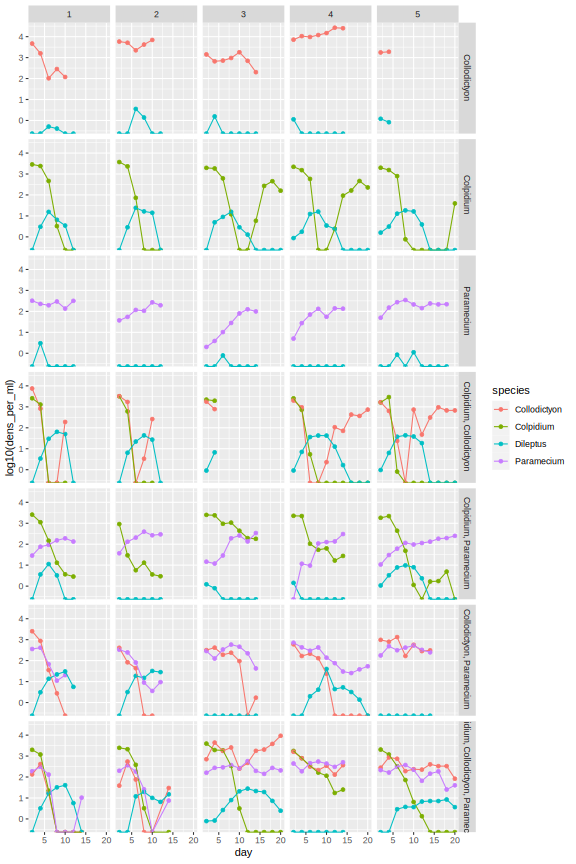
\includegraphics[width=1\linewidth]{insights_website_files/figure-latex/microbe1-1} 

}

\caption{Population dynamics observed during the experiment.}\label{fig:microbe1}
\end{figure}

\begin{info}
Notice the order of the rows---it is from top to bottom the order we
specified when we made the \texttt{prey\_composition} variable an
ordered factor. So \texttt{ggplot} is using this order. If you like to
see what the order would have been if we hadn't specified it, replace
\texttt{prey\_composition} with
\texttt{as.character(prey\_composition)}.
\end{info}

The dynamics in Figure \ref{fig:microbe1} are those shown in figure 1 of the original publication. Everything seems reasonable, though I (Owen) wish I'd recorded more information about why I stopped sampling the microcosms when I did. I think I still have my lab books from this experiment somewhere inaccessible like my parents loft but haven't had the chance to get them.

The predator (\emph{Dileptus}) does not seem to grow well when \emph{Collodictyon} is the only available prey species, but grows very well on and decimates \emph{Colpidium}, after which the predator appears to go extinct and then the \emph{Colpidium} population recovers. We can also notice that the predator population persists to the end of the experiment on day 20 only when all three prey species are present. It is probably worth emphasising that 20 days corresponds to around 20 generations of these organisms; this is a lot of time for birth and death to affect population abundances (if each individual divided into two daughters each day, the population would increase in size by a factor of 2\^{}20, i.e.~grow to be 1 million times larger).

We could again use the \texttt{skim()} function to take a look at the data more closely.

\begin{Shaded}
\begin{Highlighting}[]
\KeywordTok{skim}\NormalTok{(dd)}
\end{Highlighting}
\end{Shaded}

\begin{verbatim}
## Skim summary statistics
##  n obs: 680 
##  n variables: 12 
## 
## -- Variable type:character -----------------------
##               variable missing complete   n min max empty n_unique
##  community_composition       0      680 680  19  45     0        7
##                species       0      680 680   8  12     0        4
## 
## -- Variable type:factor --------------------------
##          variable missing complete   n n_unique
##  prey_composition       0      680 680        7
##                             top_counts ordered
##  Col: 161, Col: 108, Col: 105, Col: 98   FALSE
## 
## -- Variable type:numeric -------------------------
##       variable missing complete   n   mean      sd    p0   p25   p50
##          count       0      680 680  17.05   27.13 0      0     5   
##            day       0      680 680   8.79    5    2      4     8   
##    dens_per_ml       0      680 680 500.2  1880.55 0      0    16.41
##            jar       0      680 680  20.73   10.2  1     12    22   
##  prey_richness       0      680 680   1.93    0.73 1      1     2   
##      replicate       0      680 680   3.21    1.41 1      2     3   
##             w1       0      680 680   0.61    0.78 0.018  0.3   0.4 
##             w2       0      680 680   1.67    2.48 1      1     1   
##             w3       0      680 680   0.8     0.33 0.084  0.38  1   
##     p75     p100     hist
##   22      200    ▇▁▁▁▁▁▁▁
##   12       20    ▇▃▃▃▃▂▁▂
##  270.27 26609.54 ▇▁▁▁▁▁▁▁
##   30       35    ▃▃▃▅▂▅▅▇
##    2        3    ▆▁▁▇▁▁▁▅
##    4        5    ▆▆▁▇▁▇▁▇
##    0.81    12.22 ▇▁▁▁▁▁▁▁
##    1.96    59.24 ▇▁▁▁▁▁▁▁
##    1        2.14 ▂▁▁▇▁▁▁▁
\end{verbatim}

\hypertarget{calculate-the-three-response-variables}{%
\subsection{Calculate the three response variables}\label{calculate-the-three-response-variables}}

There are three response variables corresponding to the three hypotheses about why increased prey diversity might increase predator population stability:

\begin{itemize}
\tightlist
\item
  Predator population abundance.
\item
  Predator population variability.
\item
  Predator population persistence time.
\end{itemize}

\hypertarget{calculating-predator-dileptus-abundance}{%
\subsubsection{\texorpdfstring{Calculating predator (\emph{Dileptus}) abundance}{Calculating predator (Dileptus) abundance}}\label{calculating-predator-dileptus-abundance}}

You might be thinking ``we already have predator abundance'', and you'd be correct. We have estimates of the number per ml on each of the sample days. The issue that we now have to deal with, and solve somehow, is that of independence of observations. When we take repeated measures of the same thing, here the same predator population in the same experimental community, the repeated measures are not independent, and measures closer together in time are less independent than are those further apart in time. There are some rather complex and perhaps sophisticated ways of accounting for the non-independence in repeated measures, but they are beyond the scope of what we want to cover. Instead we are going to use a rather crude, but also quite valid solution. That is to use the maximum predator abundance in each of the experimental unit (communities). There are 35 experimental communities, so we expect to have 35 estimates of average predator abundance.

To make the calculation in R we will use a \texttt{filter\ \%\textgreater{}\%\ group\_by\ \%\textgreater{}\%\ summarise} pipeline. We filter to keep only the observations of the predator (\emph{Dileptus}), then group the data by \texttt{prey\_richness}, \texttt{prey\_composition}, and \texttt{replicate}, then calculate two summary values. The first summary value, named by us \texttt{pred\_max\_dens} is the maximum density of the predator population observed in each experimental community. The second variable calculated, named by us \texttt{all\_zero} is TRUE if all the predator densities were zero, or is otherwise FALSE. Here is the R code:

\begin{Shaded}
\begin{Highlighting}[]
\NormalTok{pred_max_dens <-}\StringTok{ }\NormalTok{dd }\OperatorTok
\StringTok{  }\KeywordTok{filter}\NormalTok{(species }\OperatorTok{==}\StringTok{ "Dileptus"}\NormalTok{) }\OperatorTok
\StringTok{  }\KeywordTok{group_by}\NormalTok{(prey_richness, prey_composition, replicate) }\OperatorTok
\StringTok{  }\KeywordTok{summarise}\NormalTok{(}\DataTypeTok{max_dens =} \KeywordTok{max}\NormalTok{(dens_per_ml),}
            \DataTypeTok{all_zero =} \KeywordTok{sum}\NormalTok{(dens_per_ml }\OperatorTok{>}\StringTok{ }\DecValTok{0}\NormalTok{) }\OperatorTok{==}\StringTok{ }\DecValTok{0}\NormalTok{) }
\end{Highlighting}
\end{Shaded}

As expected, the resulting tibble contains 35 observations and four variables. Lovely. We will look at the values after we calculate the other two response variables.

\begin{info}
In the \texttt{group\_by} we included a redundant grouping variable
\texttt{prey\_richness}. It is redundant in the sense that we would have
got the same resulting tibble if we had not included it, the only
difference being that the resulting tibble would not have contained the
\texttt{prey\_richness} variable. We will often find ourselves including
redundant variables in a \texttt{group\_by} because we would like to
them to appear in the resulting tibble so we can use them later.
\end{info}

\begin{warning}
We calculated the maximum of the predator abundance, but could have
chosen the mean, median, or the geometric mean, or harmonic mean. It is
really important to recognise that the choice of mean here is quite
arbitrary, and so introduces an element of subjectivity into our journey
from data to insights. Such subjectivity is a rather common feature of
this journey.
\end{warning}

\begin{reliability}
We must make sure our insights are robust to subjective decisions about
how to reach them. We can do this by looking at whether the insights are
sensitive to changes in these decisions. This is quite different,
however, from selecting the decision that gives a result we might
desire, which would clearly be a totally inappropriate practice.
\end{reliability}

\hypertarget{calculating-predator-dileptus-population-variability}{%
\subsubsection{\texorpdfstring{Calculating predator (\emph{Dileptus}) population variability}{Calculating predator (Dileptus) population variability}}\label{calculating-predator-dileptus-population-variability}}

We will use the coefficient of variation as the measure of predator population variable. The coefficient of variation, or CV for short, is the standard deviation of the abundances divided by the mean of the abundances. What values might we expect? Well, one thing to expect is some undefined values, since we know that in six of the communities there were no predators observed. The mean will therefore be zero, and the result of division by zero is undefined. So we expect the CV to be \texttt{NaN} for the six communities in which the predator was never observed.

The R code is very similar to that used in the previous section to calculate maximum predator abundance:

\begin{Shaded}
\begin{Highlighting}[]
\NormalTok{pred_CV <-}\StringTok{ }\NormalTok{dd }\OperatorTok
\StringTok{  }\KeywordTok{filter}\NormalTok{(species }\OperatorTok{==}\StringTok{ "Dileptus"}\NormalTok{) }\OperatorTok
\StringTok{  }\KeywordTok{group_by}\NormalTok{(prey_richness, prey_composition, replicate) }\OperatorTok
\StringTok{  }\KeywordTok{summarise}\NormalTok{(}\DataTypeTok{CV =} \KeywordTok{sd}\NormalTok{(dens_per_ml) }\OperatorTok{/}\StringTok{ }\KeywordTok{mean}\NormalTok{(dens_per_ml),}
            \DataTypeTok{all_zero =} \KeywordTok{sum}\NormalTok{(dens_per_ml }\OperatorTok{>}\StringTok{ }\DecValTok{0}\NormalTok{) }\OperatorTok{==}\StringTok{ }\DecValTok{0}\NormalTok{)}
\end{Highlighting}
\end{Shaded}

Looking at the data (e.g.~with \texttt{View(pred\_CV}) shows us that indeed there are six \texttt{NaN} values of CV. We will look at the other CV values after we calculate the third response variable.

\begin{efficiency}
\textbf{Congratulations} if you noticed that we could have calculated
maximum abundance and CV of abundance in the same summarise. This would
have been more efficient, in the sense that we would have had less code.
It would also have been safer since then we could not have accidentally
done something different (e.g.~a different grouping) for the two.
\end{efficiency}

\hypertarget{calculating-predator-dileptus-persistence-time}{%
\subsubsection{\texorpdfstring{Calculating predator (\emph{Dileptus}) persistence time}{Calculating predator (Dileptus) persistence time}}\label{calculating-predator-dileptus-persistence-time}}

Before we do, what type of variable is this? One characteristic is that it is ``time to event'' data\ldots{} we are observing the amount of time taken for a particular event (here extinction) to occur. The values can't be negative. They could be continuous, but in this case are not, because we sampled only every other day. Hence the variable is discrete numbers. We will go into a bit more detail about this nature of values of persistence time after we calculate them.

We get the last day on which \emph{Dileptus} was observed with a \texttt{filter\ \%\textgreater{}\%\ group\_by\ \%\textgreater{}\%\ summarise} pipeline. We filter to retain only observations of \emph{Dileptus} being present (i.e.~we exclude observations when \emph{Dileptus} had zero count/density per ml). Then we group the data by prey richness, prey composition, and replicate (prey richness is redundant but we want to keep it to work with later). Then we use \texttt{summarise} to get the maximum value of the \texttt{day} variable in the filtered data. Translated into R this looks like:

\begin{Shaded}
\begin{Highlighting}[]
\NormalTok{temp_persistence_time <-}\StringTok{ }\NormalTok{dd }\OperatorTok
\StringTok{  }\KeywordTok{filter}\NormalTok{(species }\OperatorTok{==}\StringTok{ "Dileptus"}\NormalTok{, dens_per_ml }\OperatorTok{!=}\StringTok{ }\DecValTok{0}\NormalTok{) }\OperatorTok
\StringTok{  }\KeywordTok{group_by}\NormalTok{(prey_richness, prey_composition, replicate) }\OperatorTok
\StringTok{  }\KeywordTok{summarise}\NormalTok{(}\DataTypeTok{last_day_observed =} \KeywordTok{max}\NormalTok{(day))}
\end{Highlighting}
\end{Shaded}

Note that the created tibble has only 29 observations, whereas there were 35 experimental communities. This difference occurs because \emph{Dileptus} was never observed in six of the experimental communities and so these are filtered out of this analysis. We will add them in below as a side effect of another manipulation, so don't need to take care of this further here.

Next we need to recognise that the last day on which \emph{Dileptus} was observed might have been the last day observed because it was after that observed to be extinct, or that it was never sampled again (e.g.~if the last day observed was day 20). If we stop an experiment before we observe the event being watched for (e.g.~before we observe extinction) then we say that the observation is \emph{censored}.

We really should include this information in the persistence time dataset. To do so we need to get and add the day of last sample of \emph{Dileptus}. We do this with the same pipeline as we used to get the last day observed, except we don't exclude the observations when \emph{Dileptus} was sampled and found to have zero abundance:

\begin{Shaded}
\begin{Highlighting}[]
\NormalTok{pred_last_day <-}\StringTok{ }\NormalTok{dd  }\OperatorTok
\StringTok{  }\KeywordTok{filter}\NormalTok{(species}\OperatorTok{==}\StringTok{"Dileptus"}\NormalTok{) }\OperatorTok
\StringTok{  }\KeywordTok{group_by}\NormalTok{(prey_richness, prey_composition, replicate) }\OperatorTok
\StringTok{  }\KeywordTok{summarise}\NormalTok{(}\DataTypeTok{last_sample=}\KeywordTok{max}\NormalTok{(day))}
\end{Highlighting}
\end{Shaded}

The created tibble has the expected number of observations: 35.

We then join the two created tibbles and create a new variable that contains \texttt{TRUE} if the observation of persistence time was censored (indicated if the persistence time is the same as the last day sampled) or \texttt{FALSE} if a sample was taken after the observed persistence time (i.e.~the observation is not censored).

\begin{Shaded}
\begin{Highlighting}[]
\NormalTok{pred_persistence_time <-}\StringTok{ }\KeywordTok{full_join}\NormalTok{(temp_persistence_time, pred_last_day) }\OperatorTok
\StringTok{  }\KeywordTok{mutate}\NormalTok{(}\DataTypeTok{censored=}\KeywordTok{ifelse}\NormalTok{(last_day_observed}\OperatorTok{==}\NormalTok{last_sample, T, F))}
\end{Highlighting}
\end{Shaded}

\begin{verbatim}
## Joining, by = c("prey_richness", "prey_composition", "replicate")
\end{verbatim}

Because we used \texttt{full\_join} we have 35 observations in the resulting tibble, with six \texttt{NA} values of persistence time (and also therefore \texttt{censored}) corresponding to the six communities that are missing from the \texttt{persistence\_time} tibble because \emph{Dileptus} was never observed in those communities.

\begin{info}
\textbf{Censored observations in time to event data} Often we do not
have the exact time at which the event of interest occurred. In this
experiment we sampled only one every two days. If we observed some
individuals on day 14, for example, and then none on or after day 16, we
know that extinction occurred somewhere in the time interval between day
14 and day 16. Thus we have what is called ``interval censored'' time to
event data. That is, unless extinction was not observed by the last
sample, in which case the data are right censored, and we can only say
that extinction (since it is at some point inevitable) will happen
sometime after the day of the last sample. Censoring of time to event
data is very common and is formally accounted for in statistical
analyses of time to event type data. It certainly complicates and adds
potential for misinterpreting visualisation of the data, so we must then
at least differentiate data points by the type of censoring they have.
\end{info}

\hypertarget{put-the-all-together}{%
\subsubsection{Put the all together}\label{put-the-all-together}}

Let's put all three response variables into the same tibble, since it will make some of the subsequent things easier and more efficient. We want them all in the same column. ``But wait'', you say! If all three response variables are in the same column/variable, how will we know which is which. Easy---we make another variable that tells us the response variable in each row. The new tibble will have 35 * 3 = 105 rows. There are lots of ways to do this. The approach we show is to merge/join the three tibbles containing each of the response variables (\texttt{pred\_max\_dens}, \texttt{pred\_CV}, and \texttt{pred\_persistence\_time}) which creates a wide-formatted arrangement of the data (a different variable for each of the response variables). And then we'll transform it into tidy (long) format by gather the information from each of the three separate response variables into one variable.

The first step is to merge all three tibbles:

\begin{Shaded}
\begin{Highlighting}[]
\NormalTok{spread_rr <-}\StringTok{ }\NormalTok{pred_max_dens }\OperatorTok
\StringTok{  }\KeywordTok{full_join}\NormalTok{(pred_CV) }\OperatorTok
\StringTok{  }\KeywordTok{full_join}\NormalTok{(pred_persistence_time)}
\end{Highlighting}
\end{Shaded}

\begin{verbatim}
## Joining, by = c("prey_richness", "prey_composition", "replicate", "all_zero")
\end{verbatim}

\begin{verbatim}
## Joining, by = c("prey_richness", "prey_composition", "replicate")
\end{verbatim}

We get told both joins are being done by \texttt{prey\_richness}, \texttt{prey\_composition}, and \texttt{replicate} and also \texttt{all\_zero} for the first of the two joins. Lovely---thanks very much. (The join is done by these because R looks for variables shared by the two tibbles being joined, and by default joins by these.)

Next step is to gather the three response variables into one variable:

\begin{Shaded}
\begin{Highlighting}[]
\NormalTok{rr <-}\StringTok{ }\NormalTok{spread_rr }\OperatorTok
\StringTok{  }\KeywordTok{gather}\NormalTok{(}\DataTypeTok{key =} \StringTok{"Response_type"}\NormalTok{, }\DataTypeTok{value =}\NormalTok{ Value, max_dens, CV, last_day_observed)}
\end{Highlighting}
\end{Shaded}

We tell \texttt{gather} that we'd like the values in the variables \texttt{max\_dens}, \texttt{CV}, and \texttt{last\_day\_observed} gathered together an put into one variable called \texttt{Values} and that we'd like the \texttt{key} variable, i.e.~the one that says which response variable each observation is about, to be named \texttt{Response\_type}. If how \texttt{gather} works is unclear then please wait until Case Study 3, where the explanation goes into more depth, including a figure showing tidy/long data and the corresponding untidy/wide data (Figure \ref{fig:long-wide}).

Excellent. We now have a tibble \texttt{rr} with 105 observations (as expected), a variable named \texttt{Response\_type} with entries \texttt{max\_dens}, \texttt{CV}, and \texttt{last\_day\_observed}, and the values of each of these in the \texttt{Value} variable. We have the other variables \texttt{all\_zero}, \texttt{last\_sample}, and \texttt{censored} also (which is just fine).

\hypertarget{shapes-1}{%
\section{Shapes}\label{shapes-1}}

Let's get the mean, standard deviation, and number of observations of each of the response variables for each prey composition. You have seen how to do this before. Take a look back through the book/your notes/your brain to remind yourself.

Yes\ldots{} it's a pretty straightforward \texttt{group\_by\ \%\textgreater{}\%\ summarise} pipeline:

\begin{Shaded}
\begin{Highlighting}[]
\NormalTok{summry_rr <-}\StringTok{ }\NormalTok{rr }\OperatorTok
\StringTok{  }\KeywordTok{group_by}\NormalTok{(prey_richness, prey_composition, Response_type) }\OperatorTok
\StringTok{  }\KeywordTok{summarise}\NormalTok{(}\DataTypeTok{mean =} \KeywordTok{mean}\NormalTok{(Value, }\DataTypeTok{na.rm =} \OtherTok{TRUE}\NormalTok{),}
            \DataTypeTok{sd =} \KeywordTok{sd}\NormalTok{(Value, }\DataTypeTok{na.rm =} \OtherTok{TRUE}\NormalTok{),}
            \DataTypeTok{n =} \KeywordTok{sum}\NormalTok{(}\OperatorTok{!}\KeywordTok{is.na}\NormalTok{(Value)))}
\end{Highlighting}
\end{Shaded}

The resulting tibble \texttt{summry\_rr} has 21 observations (7 prey compositions by 3 response variables) and six variables, three of which are the calculated mean, standard deviation, and number of non-NA values.

\begin{info}
We counted the number of non-NA values by asking which of the entries in
\texttt{Value} were not NA using \texttt{!is.na}, which gives a series
of TRUE and FALSE values. Then we use \texttt{sum} to count the number
of TRUEs.
\end{info}

Take a look at the resulting tibble (\texttt{View(summry\_rr)}). Can you see any patterns? Do you get clear insights? Probably not. The lesson here is tables are quite difficult to interpret. We need some visualisations of relationships between the response variables differ and the treatments. Before we do this, let's have a look at the distributions of the response variables. Try to think about how you would produce graphs of the frequency distributions of each of the response variables.

Here is how we did it (producing Figure \ref{fig:microbe2}):

\begin{Shaded}
\begin{Highlighting}[]
\KeywordTok{ggplot}\NormalTok{(rr, }\KeywordTok{aes}\NormalTok{(}\DataTypeTok{x =}\NormalTok{ Value)) }\OperatorTok{+}
\StringTok{  }\KeywordTok{geom_histogram}\NormalTok{(}\DataTypeTok{bins =} \DecValTok{5}\NormalTok{) }\OperatorTok{+}
\StringTok{  }\KeywordTok{facet_wrap}\NormalTok{(}\OperatorTok{~}\StringTok{ }\NormalTok{Response_type, }\DataTypeTok{scales =} \StringTok{"free"}\NormalTok{)}
\end{Highlighting}
\end{Shaded}

\begin{verbatim}
## Warning: Removed 12 rows containing non-finite values (stat_bin).
\end{verbatim}

\begin{figure}

{\centering 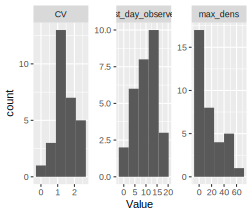
\includegraphics[width=1\linewidth]{insights_website_files/figure-latex/microbe2-1} 

}

\caption{Histograms of the three response variables.}\label{fig:microbe2}
\end{figure}

First note that we are told that 12 non-finite values have been removed and therefore are not in the visualisation. These are the \texttt{CV} and \texttt{last\_day\_observed} for the six communities were no predators were ever observed.

What do you think about the shapes of these distributions? Maximum density looks quite skewed, with lots of small values and few large. This might be expected for an abundance type variable, since growth is a multiplicative process. We would expect a more symmetric distribution of logged abundance (though see Figure \ref{fig:microbe3}).

\begin{verbatim}
## Warning: Removed 6 rows containing non-finite values (stat_bin).
\end{verbatim}

\begin{figure}

{\centering 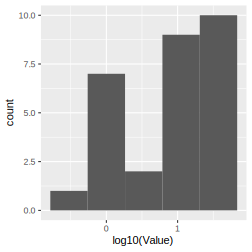
\includegraphics[width=0.7\linewidth]{insights_website_files/figure-latex/microbe3-1} 

}

\caption{Histogram of log10 maximum abundance. We thought that log transformation would make the distribution more symmetric, but it has not... it just made it asymmetric in the opposite direction!}\label{fig:microbe3}
\end{figure}

There are two reasons why we need to be cautious, however, about interpreting much about these distributions. First, they each contain data from seven different treatments (\texttt{prey\_composition})---only five of the values in each distribution might be expected to come from the same population. In effect, we might be looking at seven distributions superimposed on top of each other. Second, sure, we could plot a separate distribution for each of the prey compositions, but we would only have five values per distribution, and that is not enough to say much about their shapes. I.e. we could not say with any confidence if they are symmetric of not. All is not lost, however, as you will see in the next section in which we look at relationships.

\hypertarget{relationships-1}{%
\section{Relationships}\label{relationships-1}}

Recall the question we're interested in. Do predators have more stable populations when they have more prey to feed on. We expected this to be so if maximum predator population was greater, if predator population variability was lower, and if predator population persistence was longer when there were more prey available. For each of these we must look at the relationship between the response variable and prey richness (the explanatory variable). We can also look at prey composition as an explanatory variable, to see if there is much difference between effects of prey communities with same number of prey species, but different compositions of prey species.

\hypertarget{maximum-predator-density}{%
\subsection{Maximum predator density}\label{maximum-predator-density}}

Recall that we have one tibble \texttt{rr} with all three response variables. Clearly then, if we want to plot data about only maximum prey density we will need to filter the data according to \texttt{Response\_type\ ==\ "max\_dens}. We then do a pretty straightforward \texttt{ggplot} with \texttt{prey\_richness} mapped onto the x-axis, the \texttt{Value} of maximum density mapped onto the y-axis, and then a \texttt{geom\_jitter} with jitter only along the x-axis (\texttt{width}). Here's the code, and the result is in Figure \ref{fig:microbe4-0}:

\begin{figure}

{\centering 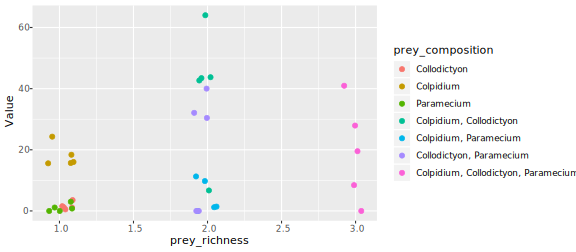
\includegraphics[width=1\linewidth]{insights_website_files/figure-latex/microbe4-0-1} 

}

\caption{A not so useful graph due to the y-axis label being totally uninformative. Value of what?}\label{fig:microbe4-0}
\end{figure}

There is a big problem with this. Our figure does not tell us what is on the y-axis (``Value'' is not particularly informative!) We could fix this by changing the y-axis like this (no figure is presented for this code):

\begin{Shaded}
\begin{Highlighting}[]
\NormalTok{rr }\OperatorTok\StringTok{ }\KeywordTok{filter}\NormalTok{(Response_type }\OperatorTok{==}\StringTok{ "max_dens"}\NormalTok{) }\OperatorTok
\StringTok{  }\KeywordTok{ggplot}\NormalTok{(}\KeywordTok{aes}\NormalTok{(}\DataTypeTok{x =}\NormalTok{ prey_richness, }\DataTypeTok{y =}\NormalTok{ Value, }\DataTypeTok{col =}\NormalTok{ prey_composition)) }\OperatorTok{+}
\StringTok{  }\KeywordTok{geom_jitter}\NormalTok{(}\DataTypeTok{width =} \FloatTok{0.1}\NormalTok{, }\DataTypeTok{height =} \DecValTok{0}\NormalTok{) }\OperatorTok{+}
\StringTok{  }\KeywordTok{ylab}\NormalTok{(}\StringTok{"max_dens"}\NormalTok{)}
\end{Highlighting}
\end{Shaded}

This is a bit dangerous, in fact, because we have to make sure we have \texttt{max\_dens} written in two places. If we accidentally to write \texttt{max\_dens} in the filter and \texttt{CV} in the \texttt{ylab} we will get no warning, no error, and have no idea we did anything wrong. We should spot the error if we carefully compare the graphs among the three different response variables, as there should be some inconsistencies (e.g.~exactly the same data plotted in two, or two with different data but the same \texttt{ylab}).

Let's do the graph so we making this error is impossible. First we define an object (we name it \texttt{rv\_oi} which is an abbreviation of ``response variable of interest'') and assign to it the name of the response variable we want to graph (\texttt{max\_dens} in this case):

\begin{Shaded}
\begin{Highlighting}[]
\NormalTok{rv_oi <-}\StringTok{ "max_dens"}
\end{Highlighting}
\end{Shaded}

Then we use the same \texttt{ggplot} code as before, but with \texttt{rv\_oi} in place of \texttt{"max\_dens"} (the resulting graph is in Figure \ref{fig:microbe4-1}):

\begin{figure}

{\centering 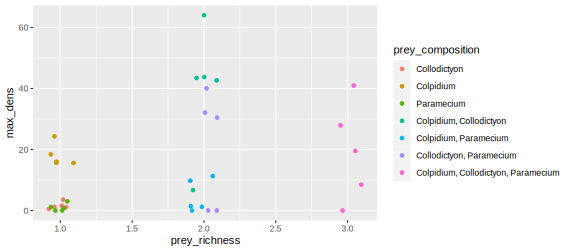
\includegraphics[width=1\linewidth]{insights_website_files/figure-latex/microbe4-1-1} 

}

\caption{A reasonably nice graph of maximum predator density in a community against the number of prey available to the predator.}\label{fig:microbe4-1}
\end{figure}

Super. We have a safe approach and a useful graph. Do you think there is strong evidence of higher maximum predator abundance at higher prey richness? Neither do we. Strike one.

\begin{reliability}
\textbf{Plot the data points} Note that we are plotting the data points,
and not bars with error bars, or even box-and-whisker plots. There are
few enough data points in this study that we experience no problems when
we plot the data itself, rather than some summary of the data (e.g.~the
mean plus and minus the standard deviation). As a rule, always plot the
data.
\end{reliability}

If we feel that we can't so easily see the differences among prey compositions within the prey richness levels, we can make Figure \ref{fig:microbe4-2}, and flip the x and y-axis since the prey composition names then fit better:

\begin{figure}

{\centering 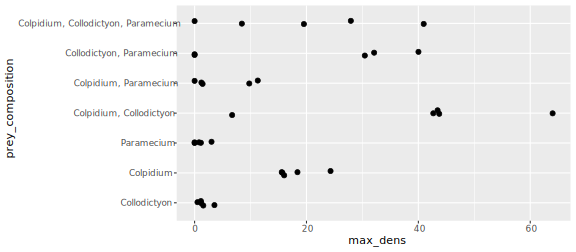
\includegraphics[width=1\linewidth]{insights_website_files/figure-latex/microbe4-2-1} 

}

\caption{This time maximum predator density plotted against prey composition, with prey composition on the y-axis as an easy method for having the tick-labels (prey composition) not overlap.}\label{fig:microbe4-2}
\end{figure}

Some things are a bit clearer. 1) The predator seems to like the prey \emph{Colpidium} when alone more than either of the other two when alone. 2) Adding \emph{Paramecium} into a mix with \emph{Colpidium} gets rid of the beneficial nature of \emph{Colpidium} (i.e.~these two act non-additively). 3) There is huge variation in predator abundance when feeding on a mixture of \emph{Colpdium} and \emph{Collodictyon}. Overall, there are strong effects of prey composition, and they sometimes involve non-additive effects, but little evidence of increases in predator abundance with increases in prey richness. Let's move on to the next response variable.

\hypertarget{predator-population-variability-cv}{%
\subsection{Predator population variability (CV)}\label{predator-population-variability-cv}}

Making the graphs for CV is now a doddle. We just set \texttt{rv\_oi\ =\ "CV} and then run exactly the same code as before, resulting in Figure \ref{fig:microbe5-1}:

\begin{verbatim}
## Warning: Removed 6 rows containing missing values (geom_point).
\end{verbatim}

\begin{figure}

{\centering 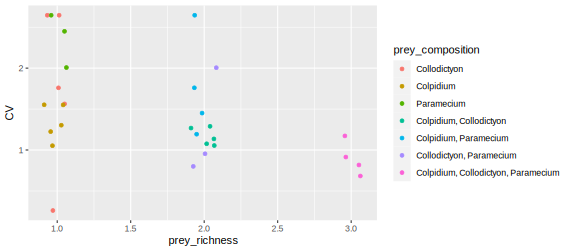
\includegraphics[width=1\linewidth]{insights_website_files/figure-latex/microbe5-1-1} 

}

\caption{A quite informative graph of predator population variability (measured as the coefficient of variation--CV) in a community against the number of prey available to the predator.}\label{fig:microbe5-1}
\end{figure}

And Figure \ref{fig:microbe5-2}:

\begin{verbatim}
## Warning: Removed 6 rows containing missing values (geom_point).
\end{verbatim}

\begin{figure}

{\centering 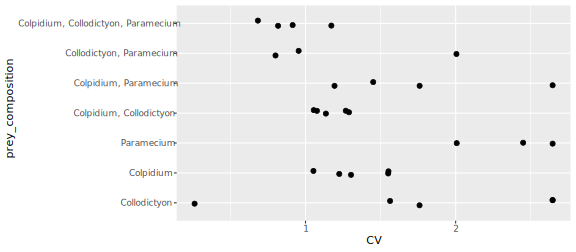
\includegraphics[width=1\linewidth]{insights_website_files/figure-latex/microbe5-2-1} 

}

\caption{Predator population variability (CV) for each of the prey compositions. It would be nice to know from which jar the very low value for one of the *Collodictyon* replicate comes. We show how to do that next.}\label{fig:microbe5-2}
\end{figure}

What do you think? Would you be confident stating that there was a negative relationship here, such that increases in prey richness cause decreases in predator population variability? Put another way, how much would you bet that in reality there is an effect? One problem here is that we have rather few data points, and quite a bit of variability even within prey compositions. Indeed, the amount of variability in the CV of the replicates of the \emph{Collodictyon} prey composition is greater than all of the other data! In large part this is due to one very low CV \emph{Collodictyon} replicate.

Looking back at Figure \ref{fig:microbe1}, can you guess which of the \emph{Collodictyon} replicates resulted in this very low CV. It is replicate 5, the one with only two samples. But this raises a couple of important points:

\begin{enumerate}
\def\labelenumi{\arabic{enumi}.}
\item
  How could be label data points in Figure \ref{fig:microbe5-2} and facets in Figure \ref{fig:microbe1} with the jar identifier, so we can directly see the corresponding data?
\item
  What if anything should we do about data points that seem rather extreme?
\end{enumerate}

Let's deal with number 1 first. We can put on the jar number as a labels on the facets of \ref{fig:microbe1} and beside the data points in Figure \ref{fig:microbe5-2}. Here's the code for putting the jar numbers onto the facets. First we get a tibble with the \texttt{jar} number for each \texttt{prey\_composition} and \texttt{replicate}, by selecting only those three columns and getting unique rows:

\begin{Shaded}
\begin{Highlighting}[]
\NormalTok{jar_text <-}\StringTok{ }\NormalTok{dd }\OperatorTok
\StringTok{  }\KeywordTok{select}\NormalTok{(prey_composition, replicate, jar) }\OperatorTok
\StringTok{  }\KeywordTok{unique}\NormalTok{()}
\end{Highlighting}
\end{Shaded}

The resulting tibble has 35 rows, one for each jar (microcosm). Then we use the same code as before but with an extra \texttt{geom\_text} in which we give the data to use \texttt{jar\_text}, tell it the x and y positions for the label, and then give the aesthetic mappings \texttt{label\ =\ jar} (i.e.~make the \texttt{label} aesthetic correspond to \texttt{jar}) and the aesthetic mapping \texttt{col\ =\ NULL} (so that the previously defined \texttt{col\ =\ species} mapping is not used). Here's the code, and the resulting graph is in Figure \ref{fig:microbe1-1}:

\begin{Shaded}
\begin{Highlighting}[]
\NormalTok{dd }\OperatorTok
\StringTok{  }\KeywordTok{ggplot}\NormalTok{(}\KeywordTok{aes}\NormalTok{(}\DataTypeTok{x =}\NormalTok{ day, }\DataTypeTok{y =} \KeywordTok{log10}\NormalTok{(dens_per_ml), }\DataTypeTok{col =}\NormalTok{ species)) }\OperatorTok{+}
\StringTok{  }\KeywordTok{geom_point}\NormalTok{() }\OperatorTok{+}\StringTok{ }
\StringTok{  }\KeywordTok{geom_line}\NormalTok{() }\OperatorTok{+}
\StringTok{  }\KeywordTok{facet_grid}\NormalTok{(prey_composition }\OperatorTok{~}\StringTok{ }\NormalTok{replicate) }\OperatorTok{+}
\StringTok{  }\KeywordTok{geom_text}\NormalTok{(}\DataTypeTok{data =}\NormalTok{ jar_text, }\DataTypeTok{x =} \DecValTok{18}\NormalTok{, }\DataTypeTok{y =} \FloatTok{3.5}\NormalTok{, }\KeywordTok{aes}\NormalTok{(}\DataTypeTok{label =}\NormalTok{ jar, }\DataTypeTok{col =} \OtherTok{NULL}\NormalTok{))}
\end{Highlighting}
\end{Shaded}

\begin{figure}

{\centering 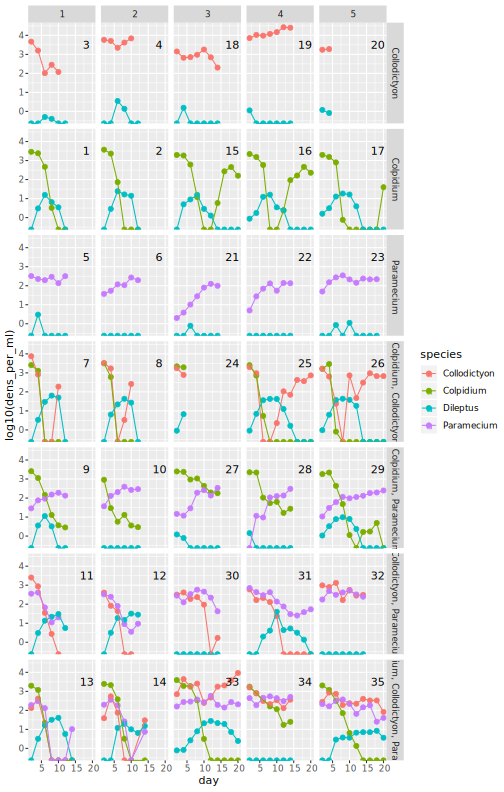
\includegraphics[width=1\linewidth]{insights_website_files/figure-latex/microbe1-1-1} 

}

\caption{Jar numbers added to the plot of population dynamics observed during the experiment.}\label{fig:microbe1-1}
\end{figure}

Next we add points to the graph of the CV (Figure \ref{fig:microbe5-2}). First we need to remake the tibble containing the CVs, this time keeping the \texttt{jar} variable by adding it as a (albeit redundant) variable in the \texttt{group\_by}:

\begin{Shaded}
\begin{Highlighting}[]
\NormalTok{pred_CV <-}\StringTok{ }\NormalTok{dd }\OperatorTok
\StringTok{  }\KeywordTok{filter}\NormalTok{(species }\OperatorTok{==}\StringTok{ "Dileptus"}\NormalTok{) }\OperatorTok
\StringTok{  }\KeywordTok{group_by}\NormalTok{(jar, prey_richness, prey_composition, replicate) }\OperatorTok
\StringTok{  }\KeywordTok{summarise}\NormalTok{(}\DataTypeTok{CV =} \KeywordTok{sd}\NormalTok{(dens_per_ml) }\OperatorTok{/}\StringTok{ }\KeywordTok{mean}\NormalTok{(dens_per_ml),}
            \DataTypeTok{all_zero =} \KeywordTok{sum}\NormalTok{(dens_per_ml }\OperatorTok{>}\StringTok{ }\DecValTok{0}\NormalTok{) }\OperatorTok{==}\StringTok{ }\DecValTok{0}\NormalTok{)}
\end{Highlighting}
\end{Shaded}

\begin{action}
Install the \textbf{ggrepel} add-on package. It moves labels on graphs
so they don't lie on top of each other, i.e.~they repel each other.
\end{action}

Now we remake the CV figure with the jar numbers labeling the data points. We simply add a \texttt{geom\_text\_repel} with the \texttt{jar} numbers mapped onto the \texttt{label} aesthetic. Here's the code, and the resulting graph is in Figure \ref{fig:microbe5-3}.

\begin{Shaded}
\begin{Highlighting}[]
\KeywordTok{library}\NormalTok{(ggrepel)}
\KeywordTok{ggplot}\NormalTok{(pred_CV, }\KeywordTok{aes}\NormalTok{(}\DataTypeTok{x =}\NormalTok{ prey_composition, }\DataTypeTok{y =}\NormalTok{ CV)) }\OperatorTok{+}
\StringTok{  }\KeywordTok{geom_jitter}\NormalTok{(}\DataTypeTok{width =} \FloatTok{0.1}\NormalTok{, }\DataTypeTok{height =} \DecValTok{0}\NormalTok{) }\OperatorTok{+}
\StringTok{  }\KeywordTok{coord_flip}\NormalTok{() }\OperatorTok{+}
\StringTok{  }\KeywordTok{geom_text_repel}\NormalTok{(}\KeywordTok{aes}\NormalTok{(}\DataTypeTok{label =}\NormalTok{ jar))}
\end{Highlighting}
\end{Shaded}

\begin{verbatim}
## Warning: Removed 6 rows containing missing values (geom_point).
\end{verbatim}

\begin{verbatim}
## Warning: Removed 6 rows containing missing values (geom_text_repel).
\end{verbatim}

\begin{figure}

{\centering 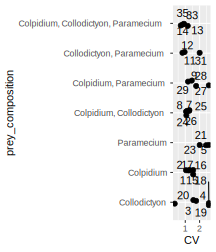
\includegraphics[width=1\linewidth]{insights_website_files/figure-latex/microbe5-3-1} 

}

\caption{Again the predator population variability data, but this time with jar numbers added as label by the data points.}\label{fig:microbe5-3}
\end{figure}

Super. It's extremely useful to be able to add labels to data point in graphs, so we can see which replicate, individual, site, etc., the data point corresponds to. This is especially useful when we see what appear to be rather extreme values, which bring us to the next general point---what can and should we do when we see what might be extreme values? Here is a checklist:

\begin{enumerate}
\def\labelenumi{\arabic{enumi}.}
\item
  Use your best judgment about if a value seems extreme. If you're in doubt, consider it extreme. Nothing we subsequently do will with these apparently extreme values will cause problems if we include some values as being extreme that other people might not.
\item
  Check that each extreme value is not the result of an error. E.g. in data entry, or subsequent assumptions in calculations. If you ever meet us in person, ask us to tell you the badger testicle size story. It involves using -9999 as the missing value indicator, calculation of testicle volume that involved squaring the measured testicle width, and some apparently very well endowed badgers.
\item
  Plot your graphs with and without the extreme values and see if this leads to you changing your opinion about the presence, absence, or nature of any patterns. If it seems that including or excluding them is important, well, that's your answer. Your conclusions are not so robust.
\item
  It's beyond the scope of this book, but still worth mentioning that there are quantitative ways to assess if data points are extreme (also known as \emph{outliers}) and if they affect quantitative conclusions (i.e.~result of statistical analyses), but ultimately all include some element of subjectivity in their use and interpretation.
\end{enumerate}

While we're on the subject of subjectivity and perception, we should think about whether flipping the axis does more than just make room for the prey composition labels. Does having the graph flipped change our perception of pattern (or lack thereof) in the data? Figure \ref{fig:microbe5-4}A and B. We (personally) tend to see more evidence of a negative relationship in panel B (with prey richness on the x-axis) but you might be different. We need to be careful to not exploit, or fall prey to, any such effects in the presentation of data. The data should, as far as possible, do all the talking.

\begin{verbatim}
## Warning: Removed 6 rows containing missing values (geom_point).

## Warning: Removed 6 rows containing missing values (geom_point).
\end{verbatim}

\begin{figure}

{\centering 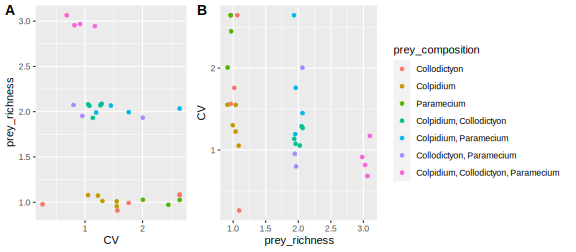
\includegraphics[width=1\linewidth]{insights_website_files/figure-latex/microbe5-4-1} 

}

\caption{The same graph twice, but with the axis flipped between them. Do you think pattern is more apparent in one versus the other?}\label{fig:microbe5-4}
\end{figure}

\hypertarget{predator-persistence-time}{%
\subsection{Predator persistence time}\label{predator-persistence-time}}

Visualising predator persistence time (the last day on which a predator was observed) uses the same code as the previous two response variables, but with one tweek. We should differentiate in the visualisation data points that are and are not censored. One method is to make their data points have different shapes. That is, we map the shape aesthetic to the \texttt{censored} variable (the resulting graph is in Figure \ref{fig:microbe7-1}):

\begin{verbatim}
## Warning: Removed 6 rows containing missing values (geom_point).
\end{verbatim}

\begin{figure}

{\centering 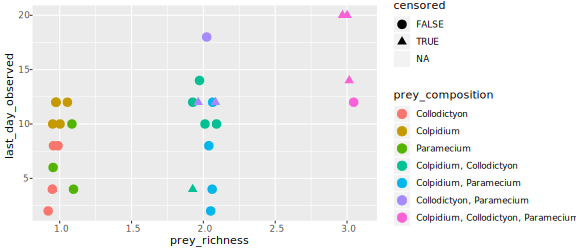
\includegraphics[width=1\linewidth]{insights_website_files/figure-latex/microbe7-1-1} 

}

\caption{A reasonably nice graph of predator population persistence time against the number of prey available to the predator.}\label{fig:microbe7-1}
\end{figure}

There is pretty strong evidence that more prey species available to a predator increases the time for which the predator population persists. With three prey species available, three of the persistence times were censored, and two of these were censored after 20 days---the longest of any population observed. There isn't such a clear difference between persistence times between one and two prey communities.

We also show, as before, the same data for each prey composition, again showing which observations of persistence time are censored (the resulting graph is in Figure \ref{fig:microbe7-2}):

\begin{figure}

{\centering 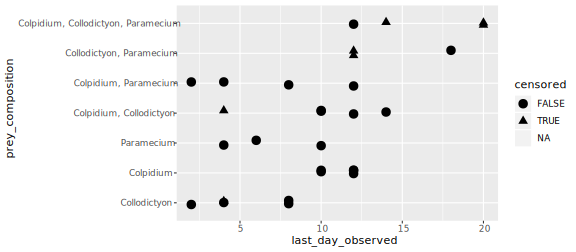
\includegraphics[width=1\linewidth]{insights_website_files/figure-latex/microbe7-2-1} 

}

\caption{Predator population persistence time for each of the prey compositions.}\label{fig:microbe7-2}
\end{figure}

Here we can see that one of the two prey species compositions (\emph{Collodictyon} and \emph{Paramecium}) results in predator persistence times as long as with three prey species. And that one of the one prey species composition (\emph{Colpidium}) results in persistence times as long as some of the two prey species compositions. So there are quite strong compositional effects as well as the richness effect mentioned above.

\begin{efficiency}
Look at Figure \ref{fig:microbe6-3} showing what happens if
\texttt{prey\_composition} is just a character variable and not an
ordered factor. The ordering of the prey compositions is not quite as
desirable.
\end{efficiency}

\begin{figure}

{\centering 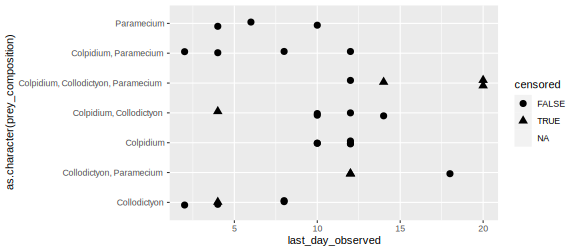
\includegraphics[width=1\linewidth]{insights_website_files/figure-latex/microbe6-3-1} 

}

\caption{Notice how the prey compositions are ordered when we let R choose the order. This happens when we fail to specify ourselves what the order should be, by making the prey composition variable an ordered factor type variable.}\label{fig:microbe6-3}
\end{figure}

\hypertarget{all-three-at-once}{%
\subsection{All three at once}\label{all-three-at-once}}

You might be wondering why we went to the lengths of putting all three response variables into one tibble and the having to filter in order to plot each of the three graphs. This was a bit of a faff. We could have just continued using the three separate tibbles we made. Here comes the answer, or at least here comes one answer. If we put all three response variables into the same tibble the we can plot all three graphs at the same time, in one ggplot with three facets (Figure \ref{fig:microbe8-1}):

\begin{Shaded}
\begin{Highlighting}[]
\NormalTok{rr }\OperatorTok
\StringTok{  }\KeywordTok{ggplot}\NormalTok{(}\KeywordTok{aes}\NormalTok{(}\DataTypeTok{x =}\NormalTok{ prey_richness, }\DataTypeTok{y =}\NormalTok{ Value, }\DataTypeTok{col =}\NormalTok{ prey_composition)) }\OperatorTok{+}
\StringTok{  }\KeywordTok{geom_jitter}\NormalTok{(}\DataTypeTok{width =} \FloatTok{0.1}\NormalTok{, }\DataTypeTok{height =} \DecValTok{0}\NormalTok{) }\OperatorTok{+}
\StringTok{  }\KeywordTok{facet_wrap}\NormalTok{(}\OperatorTok{~}\StringTok{ }\NormalTok{Response_type, }\DataTypeTok{scales =} \StringTok{"free_y"}\NormalTok{)  }\OperatorTok{+}
\StringTok{  }\KeywordTok{theme}\NormalTok{(}\DataTypeTok{legend.position =} \StringTok{"top"}\NormalTok{) }\OperatorTok{+}
\StringTok{  }\KeywordTok{guides}\NormalTok{(}\DataTypeTok{colour =} \KeywordTok{guide_legend}\NormalTok{(}\DataTypeTok{title.position =} \StringTok{"top"}\NormalTok{,}
                               \DataTypeTok{nrow =} \DecValTok{3}\NormalTok{,}
                               \DataTypeTok{position =} \StringTok{"top"}\NormalTok{))}
\end{Highlighting}
\end{Shaded}

\begin{verbatim}
## Warning: Removed 12 rows containing missing values (geom_point).
\end{verbatim}

\begin{figure}

{\centering 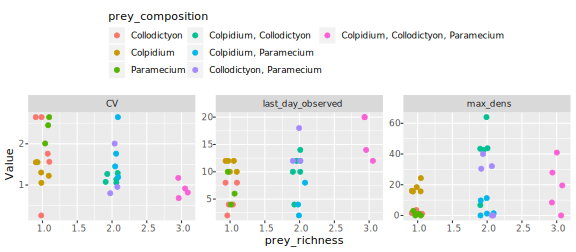
\includegraphics[width=1\linewidth]{insights_website_files/figure-latex/microbe8-1-1} 

}

\caption{All three reponse variables efficiently made in one call to ggplot with a facet for each variable, and some fiddling with the legend to get it at the top and not too wide.}\label{fig:microbe8-1}
\end{figure}

How useful is it to be able to plot all response variables in one go like this? We're not too sure. We now have the problem of how to show the censored data points in the \texttt{last\_day\_observed} data. We also see that the order of the facets is different from the order of the response variables presented in the text above. This would need changing for consistency (you can probably guess how we would do this\ldots{} the same thing we did with the \texttt{prey\_composition} variable). We'll leave this for you to do. And also to make the version of this graph with \texttt{prey\_composition} as the explanatory variable.

\hypertarget{wrapping-up-1}{%
\section{Wrapping up}\label{wrapping-up-1}}

The published paper on this dataset had a few other analyses, but not too many. So what you learned above is very much a replica of a real and quite complete representation of the results and insights in the that study. Yes, we didn't do the statistics, but our conclusions are pretty much the same (though this could easily be in part influenced by Owen knowing in the conclusions before he wrote this chapter).

One important thing. It would be very very wrong for you to get the impression that one can think through all the likely issues with the data and in a lovely linear process work from the data to the Insights. Probably this impression comes from this chapter and those of the first case study. For example, we do things early on in the data manipulation in order to make things easier later on. It looks like we anticipate a problem that will arise and prevent it ever occurring.

The truth is, however, that we often found problems once we had got quite far into the data processing, and then realised we should go back and fix their cause. E.g. we found a problem while plotting the data, realised this was caused by an issue that could be sorted out much earlier on, and therefore have positive effects on all subsequent analyses. We did not just do a quick fix on the problematic graph\ldots{} we fixed the source of the problem. This is a very very good habit to get into. Fix the cause, don't just treat the symptom. Fixing the cause will increase efficiency, reliability, and all round happiness.

\hypertarget{some-questions-1}{%
\section{Some questions}\label{some-questions-1}}

Go to the Insights companion website \url{http://insightsfromdata.io} and have a go at the questions and exercises for this chapter.

\hypertarget{WFD-4}{%
\chapter{Effects of dietary restriction}\label{WFD-4}}

\begin{Shaded}
\begin{Highlighting}[]
\CommentTok{## Load the libraries we use}
\KeywordTok{library}\NormalTok{(dplyr)}
\KeywordTok{library}\NormalTok{(ggplot2)}
\KeywordTok{library}\NormalTok{(readr)}
\KeywordTok{library}\NormalTok{(stringr)}
\KeywordTok{library}\NormalTok{(lubridate)}
\KeywordTok{library}\NormalTok{(skimr)}
\KeywordTok{library}\NormalTok{(tidyr)}
\KeywordTok{library}\NormalTok{(ggbeeswarm)}
\KeywordTok{library}\NormalTok{(taxize)}
\KeywordTok{library}\NormalTok{(broom)}
\KeywordTok{library}\NormalTok{(forcats)}
\end{Highlighting}
\end{Shaded}

A general article about dietary restriction (DR): \url{https://www.nia.nih.gov/health/calorie-restriction-and-fasting-diets-what-do-we-know}

The case study article: \emph{Reconciling nutritional geometry with classical dietary restriction: effects of nutrient intake, not calories, on survival and reproduction.} Moatt JP, Fyfe MA, Heap E, Mitchell LJM, Moon F, Walling CA (2018) Aging Cell, Volume 18, e12868.

Article: \url{https://doi.org/10.1111/acel.12868}

Data: \url{https://doi.org/10.5061/dryad.g12p0j2}

Abstract: ``Here, using a novel nonmodel vertebrate system (the stickleback fish, \emph{Gasterosteus aculeatus}), we test the effect of macronutrient versus calorie intake on key fitness‐related traits, both using the GF and avoiding dietary dilution. We find that the intake of macronutrients rather than calories determines both mortality risk and reproduction. Male mortality risk was lowest on intermediate lipid intakes, and female risk was generally reduced by low protein intakes. The effect of macronutrient intake on reproduction was similar between the sexes, with high protein intakes maximizing reproduction.''

\hypertarget{before-working-in-r}{%
\section{Before working in R}\label{before-working-in-r}}

\textbf{Question}: How does diet composition and amount of food individually and in combination affect individual characteristics related to health and fitness?

\textbf{Hypotheses/predictions}:

\begin{itemize}
\tightlist
\item
  Fitness: ``mortality''
\item
  Fitness: ``reproductive behaviour (time spent courting)''
\item
  Fitness: ``Female reproduction (total egg production)''
\item
  Health: ``We use change in fish length as our measure of growth.''
\item
  Health: ``As a proxy for overall health, we use body condition index, which is a measure of the weight of an individual relative to its length''
\end{itemize}

\textbf{Study methods and design} (\textbf{numbers of ``things''}) ``We fed 300 male and 300 female individually housed three‐spine sticklebacks one of five diets varying in protein and lipid content (Table 2) at one of three provisioning levels (100\%, 75\% or 50\% of ad lib), therefore using a restriction of food availability rather than a dilution of the diets to achieve calorie restriction. This gave a total of 15 dietary treatments (see methods and supplementary materials for full details). Fish were maintained on diets for life and measured for numerous traits including survival, reproductive investment, growth and body condition. Given the broad range of traits examined, we present data for each trait separately, with an accompanying short interpretation section.''

``Mortality was checked twice daily and date of death was recorded. We quantified male lifetime reproductive investment as the total time spent courting (in seconds) across all courtship attempts. Males were also assayed for other common reproductive behaviours (e.g., territory defence, nesting and nuptial coloration---see supplementary methods and analysis). Female lifetime reproductive investment was taken as the total number of eggs produced). Fish were monitored for growth (length (mm) and weight (g)) approximately every 1--2 months (Supporting Information Table S26). From these measures, body condition (overall health) was also quantified (Moatt et al., 2017 and supplementary methods).''

Q: How many fish per treatment combination? A. 20

\textbf{Type of response variable:}

\begin{itemize}
\tightlist
\item
  Mortality---binary, dead or alive.
\item
  Time spent courting---cannot be negative, will likely be numeric, may be distrete (e.g.~10 mins or 20 minutes) or continuous, ratio type.
\item
  Female reproduction egg production---count type data, not negative, discrete (integers), ratio type.
\item
  Change in fish length---could be negative or positive, ratio type.
\item
  Body condition index (a measure of the weight of an individual relative to its length)-only positive, likely continuous, ratio type.
\end{itemize}

\textbf{Explanatory variables:}

\begin{itemize}
\tightlist
\item
  A variable about the diet composition treatment.
\item
  A variable about the provisioning level treatment.
\item
  Perhaps some others.
\end{itemize}

\textbf{Predictions}:
What were the predictions?

\textbf{Data birth}:

\begin{itemize}
\tightlist
\item
  \textbf{Number of variables}: not too many as a designed experiment with clear question.
\item
  \textbf{Number of observations}: number of fish (they were ``individually housed'', and assigned treatment on an individual level).
\item
  \textbf{Variables describing manipulations}: yes, two.
\item
  \textbf{Correlation among variables}: low (factorial experiment, though some imbalance likely)
\item
  \textbf{Independence of observations}: there may be multiple observations per fish (repeated measures). Fish may share mothers, fathers, and other pre-experiment conditions.
\end{itemize}

\textbf{Secure resources and perform study}

\textbf{Which datafiles:} Have a look at the data files on the dryad repository. Which data files are required for which response variable?

\begin{Shaded}
\begin{Highlighting}[]
\NormalTok{mortality <-}\StringTok{ }\KeywordTok{read_csv}\NormalTok{(}\StringTok{"data/Moatt_et_al_Data_S1.csv"}\NormalTok{)}
\end{Highlighting}
\end{Shaded}

\begin{verbatim}
## Parsed with column specification:
## cols(
##   .default = col_double(),
##   FID = col_character(),
##   Sex = col_character(),
##   Size = col_character()
## )
\end{verbatim}

\begin{verbatim}
## See spec(...) for full column specifications.
\end{verbatim}

\begin{Shaded}
\begin{Highlighting}[]
\NormalTok{courtship <-}\StringTok{ }\KeywordTok{read_csv}\NormalTok{(}\StringTok{"data/Moatt_et_al_Data_S5.csv"}\NormalTok{)}
\end{Highlighting}
\end{Shaded}

\begin{verbatim}
## Parsed with column specification:
## cols(
##   FID = col_character(),
##   Family = col_character(),
##   Shelf_stack = col_character(),
##   Diet = col_double(),
##   Level = col_double(),
##   Size = col_character(),
##   Trial = col_double(),
##   Days_breeding = col_double(),
##   P_day = col_double(),
##   P2_day = col_double(),
##   L_day = col_double(),
##   L2_day = col_double(),
##   Mean_react = col_double(),
##   Total_ZZ = col_double(),
##   Total_lead = col_double(),
##   Total_court = col_double()
## )
\end{verbatim}

\begin{Shaded}
\begin{Highlighting}[]
\NormalTok{eggs <-}\StringTok{ }\KeywordTok{read_csv}\NormalTok{(}\StringTok{"data/Moatt_et_al_Data_S6.csv"}\NormalTok{)}
\end{Highlighting}
\end{Shaded}

\begin{verbatim}
## Parsed with column specification:
## cols(
##   FID = col_character(),
##   Family = col_character(),
##   Stack_shelf = col_character(),
##   Diet = col_double(),
##   Level = col_double(),
##   Size = col_character(),
##   P_day = col_double(),
##   P2_day = col_double(),
##   L_day = col_double(),
##   L2_day = col_double(),
##   Days_breeding = col_double(),
##   Number_clutches = col_double(),
##   mean_number = col_double(),
##   Total_egg = col_double()
## )
\end{verbatim}

\begin{Shaded}
\begin{Highlighting}[]
\NormalTok{length_weight_condition <-}\StringTok{ }\KeywordTok{read_csv}\NormalTok{(}\StringTok{"data/Moatt_et_al_Data_S15.csv"}\NormalTok{)}
\end{Highlighting}
\end{Shaded}

\begin{verbatim}
## Parsed with column specification:
## cols(
##   FID = col_character(),
##   Shelf_stack = col_character(),
##   Sex = col_character(),
##   Diet = col_double(),
##   Level = col_double(),
##   Size = col_character(),
##   Batch = col_double(),
##   P_day = col_double(),
##   P2_day = col_double(),
##   L_day = col_double(),
##   L2_day = col_double(),
##   ZP = col_double(),
##   ZP2 = col_double(),
##   ZL = col_double(),
##   ZL2 = col_double(),
##   Ln = col_double(),
##   Wt = col_double(),
##   CI = col_double()
## )
\end{verbatim}

\textbf{Variables in the datafiles}: Look at the \texttt{data\ file\ key} word document in the dryad repository.

Which variables tell us about the experimental design (including the explantory variables) and when observations were made?

\begin{itemize}
\tightlist
\item
  \textbf{FID} -- Unique ID for each individual.
\item
  \textbf{Diet} -- Diet Treatment (Diet P:L: 1 = 10.2:1, 2 = 4.6:1, 3 = 2.5:1, 4 = 8.5:1, 5 = 1.6:1).
\item
  \textbf{Sex} -- Sex of individual (M = male, F = female).
\item
  \textbf{Size} -- Size classification of individual (L = large, S = Small).
\item
  \textbf{Level} -- Provisioning level, values represent percentages of monthly ad libitum monitoring.
\item
  \textbf{Week\_F} -- Experimental week.
\item
  \textbf{Batch} -- Weighing batch.
\end{itemize}

There are numerous other variables in the datasets. We will look at them if and when we need to.

Which variables in which dataset can be used to calculate each of the five response variables?

\begin{itemize}
\tightlist
\item
  Mortality: \texttt{status}, 0 = alive, 1 = Dead, in \texttt{Moatt\_et\_al\_Data\_S1.csv}
\item
  Time spent courting: \texttt{Total\_court} -- Total time courting across all trials, in \texttt{Moatt\_et\_al\_Data\_S5.csv}.
\item
  Female reproduction egg production: \texttt{Total\_egg} -- Total number of eggs produced, in \texttt{Moatt\_et\_al\_Data\_S6.csv}.
\item
  Change in fish length: Ln -- Length of individual in mm, in \texttt{Moatt\_et\_al\_Data\_S15.csv}.
\item
  Body condition index: CI -- Condition Index for each individual, \texttt{Moatt\_et\_al\_Data\_S15.csv}.
\end{itemize}

\textbf{Number of rows and columns in the dataset}:
(By looking at the datasets in a spreadsheet programme)

\begin{itemize}
\tightlist
\item
  \texttt{Moatt\_et\_al\_Data\_S1.csv}: 33'049 rows, 24 variables
\item
  \texttt{Moatt\_et\_al\_Data\_S5.csv}: 228, 16
\item
  \texttt{Moatt\_et\_al\_Data\_S6.csv}: 269, 14
\item
  \texttt{Moatt\_et\_al\_Data\_S15.csv}:6000, 18
\end{itemize}

\hypertarget{after-importing-the-data-into-r}{%
\section{After importing the data into R}\label{after-importing-the-data-into-r}}

\begin{itemize}
\tightlist
\item
  number of rows and columns: as expected
\item
  tidy: all four datasets appear tidy, at the moment.
\item
  variable types: all as expected
\item
  fix dates: none present
\end{itemize}

\textbf{Make more informative variable names (and discard variables not obviously of use)}:

\begin{Shaded}
\begin{Highlighting}[]
\NormalTok{courtship <-}\StringTok{ }\NormalTok{courtship }\OperatorTok
\StringTok{  }\KeywordTok{select}\NormalTok{(}\DataTypeTok{Fish_ID=}\NormalTok{FID, Family, Shelf_stack, }\DataTypeTok{Diet_comp=}\NormalTok{Diet,}
         \DataTypeTok{Prov_level=}\NormalTok{Level, }\DataTypeTok{Fish_size=}\NormalTok{Size, Trial, Total_court)}
\NormalTok{eggs <-}\StringTok{ }\NormalTok{eggs }\OperatorTok
\StringTok{  }\KeywordTok{select}\NormalTok{(}\DataTypeTok{Fish_ID=}\NormalTok{FID, Family, }\DataTypeTok{Shelf_stack=}\NormalTok{Stack_shelf, }\DataTypeTok{Diet_comp=}\NormalTok{Diet,}
         \DataTypeTok{Prov_level=}\NormalTok{Level, }\DataTypeTok{Fish_size=}\NormalTok{Size, Total_egg)}
\NormalTok{length_weight_condition <-}\StringTok{ }\NormalTok{length_weight_condition }\OperatorTok
\StringTok{  }\KeywordTok{select}\NormalTok{(}\DataTypeTok{Fish_ID=}\NormalTok{FID, Shelf_stack, }\DataTypeTok{Diet_comp=}\NormalTok{Diet, }\DataTypeTok{Sex=}\NormalTok{Sex,}
\NormalTok{         Batch,}
         \DataTypeTok{Prov_level=}\NormalTok{Level, }\DataTypeTok{Fish_size=}\NormalTok{Size, }\DataTypeTok{Length=}\NormalTok{Ln, }\DataTypeTok{Weigth=}\NormalTok{Wt, }\DataTypeTok{Cond_index=}\NormalTok{CI)}
\NormalTok{mortality <-}\StringTok{ }\NormalTok{mortality }\OperatorTok
\StringTok{  }\KeywordTok{select}\NormalTok{(}\DataTypeTok{Fish_ID=}\NormalTok{FID, }\DataTypeTok{Diet_comp=}\NormalTok{Diet, Sex,}
         \DataTypeTok{Prov_level=}\NormalTok{Level, }\DataTypeTok{Fish_size=}\NormalTok{Size, }\DataTypeTok{Week=}\NormalTok{Week_F, Status)}
\end{Highlighting}
\end{Shaded}

\textbf{Replace codes with informative words}:

\begin{Shaded}
\begin{Highlighting}[]
\NormalTok{courtship <-}\StringTok{ }\NormalTok{courtship }\OperatorTok
\StringTok{  }\KeywordTok{mutate}\NormalTok{(}\DataTypeTok{Diet_comp =} \KeywordTok{case_when}\NormalTok{(Diet_comp }\OperatorTok{==}\StringTok{ }\DecValTok{1} \OperatorTok{~}\StringTok{ "10.2:1"}\NormalTok{,}
\NormalTok{                               Diet_comp }\OperatorTok{==}\StringTok{ }\DecValTok{2} \OperatorTok{~}\StringTok{ "4.6:1"}\NormalTok{,}
\NormalTok{                               Diet_comp }\OperatorTok{==}\StringTok{ }\DecValTok{3} \OperatorTok{~}\StringTok{ "2.5:1"}\NormalTok{,}
\NormalTok{                               Diet_comp }\OperatorTok{==}\StringTok{ }\DecValTok{4} \OperatorTok{~}\StringTok{ "8.5:1"}\NormalTok{,}
\NormalTok{                               Diet_comp }\OperatorTok{==}\StringTok{ }\DecValTok{5} \OperatorTok{~}\StringTok{ "1.6:1"}\NormalTok{),}
         \DataTypeTok{Fish_size =} \KeywordTok{case_when}\NormalTok{(Fish_size }\OperatorTok{==}\StringTok{ "S"} \OperatorTok{~}\StringTok{ "Small"}\NormalTok{,}
\NormalTok{                               Fish_size }\OperatorTok{==}\StringTok{ "L"} \OperatorTok{~}\StringTok{ "Large"}\NormalTok{))}

\NormalTok{eggs <-}\StringTok{ }\NormalTok{eggs }\OperatorTok
\StringTok{  }\KeywordTok{mutate}\NormalTok{(}\DataTypeTok{Diet_comp =} \KeywordTok{case_when}\NormalTok{(Diet_comp }\OperatorTok{==}\StringTok{ }\DecValTok{1} \OperatorTok{~}\StringTok{ "10.2:1"}\NormalTok{,}
\NormalTok{                               Diet_comp }\OperatorTok{==}\StringTok{ }\DecValTok{2} \OperatorTok{~}\StringTok{ "4.6:1"}\NormalTok{,}
\NormalTok{                               Diet_comp }\OperatorTok{==}\StringTok{ }\DecValTok{3} \OperatorTok{~}\StringTok{ "2.5:1"}\NormalTok{,}
\NormalTok{                               Diet_comp }\OperatorTok{==}\StringTok{ }\DecValTok{4} \OperatorTok{~}\StringTok{ "8.5:1"}\NormalTok{,}
\NormalTok{                               Diet_comp }\OperatorTok{==}\StringTok{ }\DecValTok{5} \OperatorTok{~}\StringTok{ "1.6:1"}\NormalTok{),}
         \DataTypeTok{Fish_size =} \KeywordTok{case_when}\NormalTok{(Fish_size }\OperatorTok{==}\StringTok{ "S"} \OperatorTok{~}\StringTok{ "Small"}\NormalTok{,}
\NormalTok{                               Fish_size }\OperatorTok{==}\StringTok{ "L"} \OperatorTok{~}\StringTok{ "Large"}\NormalTok{))}

\NormalTok{length_weight_condition <-}\StringTok{ }\NormalTok{length_weight_condition }\OperatorTok
\StringTok{  }\KeywordTok{mutate}\NormalTok{(}\DataTypeTok{Diet_comp =} \KeywordTok{case_when}\NormalTok{(Diet_comp }\OperatorTok{==}\StringTok{ }\DecValTok{1} \OperatorTok{~}\StringTok{ "10.2:1"}\NormalTok{,}
\NormalTok{                               Diet_comp }\OperatorTok{==}\StringTok{ }\DecValTok{2} \OperatorTok{~}\StringTok{ "4.6:1"}\NormalTok{,}
\NormalTok{                               Diet_comp }\OperatorTok{==}\StringTok{ }\DecValTok{3} \OperatorTok{~}\StringTok{ "2.5:1"}\NormalTok{,}
\NormalTok{                               Diet_comp }\OperatorTok{==}\StringTok{ }\DecValTok{4} \OperatorTok{~}\StringTok{ "8.5:1"}\NormalTok{,}
\NormalTok{                               Diet_comp }\OperatorTok{==}\StringTok{ }\DecValTok{5} \OperatorTok{~}\StringTok{ "1.6:1"}\NormalTok{),}
         \DataTypeTok{Fish_size =} \KeywordTok{case_when}\NormalTok{(Fish_size }\OperatorTok{==}\StringTok{ "S"} \OperatorTok{~}\StringTok{ "Small"}\NormalTok{,}
\NormalTok{                               Fish_size }\OperatorTok{==}\StringTok{ "L"} \OperatorTok{~}\StringTok{ "Large"}\NormalTok{),}
         \DataTypeTok{Sex =} \KeywordTok{case_when}\NormalTok{(Sex }\OperatorTok{==}\StringTok{ "M"} \OperatorTok{~}\StringTok{ "Male"}\NormalTok{,}
\NormalTok{                         Sex }\OperatorTok{==}\StringTok{ "F"} \OperatorTok{~}\StringTok{ "Female"}\NormalTok{))}

\NormalTok{mortality <-}\StringTok{ }\NormalTok{mortality }\OperatorTok
\StringTok{  }\KeywordTok{mutate}\NormalTok{(}\DataTypeTok{Diet_comp =} \KeywordTok{case_when}\NormalTok{(Diet_comp }\OperatorTok{==}\StringTok{ }\DecValTok{1} \OperatorTok{~}\StringTok{ "10.2:1"}\NormalTok{,}
\NormalTok{                               Diet_comp }\OperatorTok{==}\StringTok{ }\DecValTok{2} \OperatorTok{~}\StringTok{ "4.6:1"}\NormalTok{,}
\NormalTok{                               Diet_comp }\OperatorTok{==}\StringTok{ }\DecValTok{3} \OperatorTok{~}\StringTok{ "2.5:1"}\NormalTok{,}
\NormalTok{                               Diet_comp }\OperatorTok{==}\StringTok{ }\DecValTok{4} \OperatorTok{~}\StringTok{ "8.5:1"}\NormalTok{,}
\NormalTok{                               Diet_comp }\OperatorTok{==}\StringTok{ }\DecValTok{5} \OperatorTok{~}\StringTok{ "1.6:1"}\NormalTok{),}
         \DataTypeTok{Fish_size =} \KeywordTok{case_when}\NormalTok{(Fish_size }\OperatorTok{==}\StringTok{ "S"} \OperatorTok{~}\StringTok{ "Small"}\NormalTok{,}
\NormalTok{                               Fish_size }\OperatorTok{==}\StringTok{ "L"} \OperatorTok{~}\StringTok{ "Large"}\NormalTok{),}
         \DataTypeTok{Sex =} \KeywordTok{case_when}\NormalTok{(Sex }\OperatorTok{==}\StringTok{ "M"} \OperatorTok{~}\StringTok{ "Male"}\NormalTok{,}
\NormalTok{                         Sex }\OperatorTok{==}\StringTok{ "F"} \OperatorTok{~}\StringTok{ "Female"}\NormalTok{),}
         \DataTypeTok{Status =} \KeywordTok{case_when}\NormalTok{(Status }\OperatorTok{==}\StringTok{ }\DecValTok{0} \OperatorTok{~}\StringTok{ "alive"}\NormalTok{,}
\NormalTok{                            Status }\OperatorTok{==}\StringTok{ }\DecValTok{1} \OperatorTok{~}\StringTok{ "dead"}\NormalTok{))}
\end{Highlighting}
\end{Shaded}

\hypertarget{checking-for-duplicates}{%
\subsection{Checking for duplicates}\label{checking-for-duplicates}}

Question: which of the four datasets contains an odd duplicate entry? And which fish is involved? What should we do next?

\begin{Shaded}
\begin{Highlighting}[]
\KeywordTok{sum}\NormalTok{(}\KeywordTok{duplicated}\NormalTok{(}\KeywordTok{select}\NormalTok{(courtship, Fish_ID)))}
\end{Highlighting}
\end{Shaded}

\begin{verbatim}
## [1] 0
\end{verbatim}

\begin{Shaded}
\begin{Highlighting}[]
\KeywordTok{sum}\NormalTok{(}\KeywordTok{duplicated}\NormalTok{(}\KeywordTok{select}\NormalTok{(eggs, Fish_ID)))}
\end{Highlighting}
\end{Shaded}

\begin{verbatim}
## [1] 0
\end{verbatim}

\begin{Shaded}
\begin{Highlighting}[]
\KeywordTok{sum}\NormalTok{(}\KeywordTok{duplicated}\NormalTok{(}\KeywordTok{select}\NormalTok{(length_weight_condition, Fish_ID, Batch)))}
\end{Highlighting}
\end{Shaded}

\begin{verbatim}
## [1] 0
\end{verbatim}

\begin{Shaded}
\begin{Highlighting}[]
\KeywordTok{sum}\NormalTok{(}\KeywordTok{duplicated}\NormalTok{(}\KeywordTok{select}\NormalTok{(mortality, Fish_ID, Week)))}
\end{Highlighting}
\end{Shaded}

\begin{verbatim}
## [1] 1
\end{verbatim}

\begin{Shaded}
\begin{Highlighting}[]
\NormalTok{dupl <-}\StringTok{ }\KeywordTok{duplicated}\NormalTok{(}\KeywordTok{select}\NormalTok{(mortality, Fish_ID, Week))}
\KeywordTok{filter}\NormalTok{(mortality, dupl)}
\end{Highlighting}
\end{Shaded}

\begin{verbatim}
## # A tibble: 1 x 7
##   Fish_ID Diet_comp Sex   Prov_level Fish_size  Week Status
##   <chr>   <chr>     <chr>      <dbl> <chr>     <dbl> <chr> 
## 1 LR504   1.6:1     Male         100 Small         2 alive
\end{verbatim}

\begin{Shaded}
\begin{Highlighting}[]
\KeywordTok{filter}\NormalTok{(mortality, Fish_ID}\OperatorTok{==}\StringTok{"LR504"}\NormalTok{, Week}\OperatorTok{==}\DecValTok{2}\NormalTok{)}
\end{Highlighting}
\end{Shaded}

\begin{verbatim}
## # A tibble: 2 x 7
##   Fish_ID Diet_comp Sex   Prov_level Fish_size  Week Status
##   <chr>   <chr>     <chr>      <dbl> <chr>     <dbl> <chr> 
## 1 LR504   1.6:1     Male         100 Small         2 dead  
## 2 LR504   1.6:1     Male         100 Small         2 alive
\end{verbatim}

\begin{Shaded}
\begin{Highlighting}[]
\KeywordTok{filter}\NormalTok{(mortality, Fish_ID}\OperatorTok{==}\StringTok{"LR504"}\NormalTok{)}
\end{Highlighting}
\end{Shaded}

\begin{verbatim}
## # A tibble: 4 x 7
##   Fish_ID Diet_comp Sex   Prov_level Fish_size  Week Status
##   <chr>   <chr>     <chr>      <dbl> <chr>     <dbl> <chr> 
## 1 LR504   1.6:1     Male         100 Small         1 alive 
## 2 LR504   1.6:1     Male         100 Small         2 dead  
## 3 LR504   1.6:1     Male         100 Small         2 alive 
## 4 LR504   1.6:1     Male         100 Small         4 dead
\end{verbatim}

\hypertarget{nas-variable-entries-e.g.levels-of-characters-ranges-of-numerics-numbers-of-things}{%
\subsection{NAs, variable entries, e.g.~levels of characters, ranges of numerics, numbers of ``things''*}\label{nas-variable-entries-e.g.levels-of-characters-ranges-of-numerics-numbers-of-things}}

How many missing values in the courtship dataset (remember to reduce the variables to those mentioned above)?

Which variable(s) contain missing values?

Which fish have missing values?

How many different entries are there in the \texttt{Shelf\_stack} variable?

What are the mean and median of the \texttt{Total\_court} variable?

What are the units of the \texttt{Total\_court} variable? (From paper only, seconds)

\begin{Shaded}
\begin{Highlighting}[]
\KeywordTok{skim}\NormalTok{(courtship)}
\end{Highlighting}
\end{Shaded}

\begin{verbatim}
## Skim summary statistics
##  n obs: 228 
##  n variables: 8 
## 
## -- Variable type:character -----------------------
##     variable missing complete   n min max empty n_unique
##    Diet_comp       0      228 228   5   6     0        5
##       Family       0      228 228   4   4     0       22
##      Fish_ID       0      228 228   5   5     0      228
##    Fish_size       0      228 228   5   5     0        2
##  Shelf_stack       0      228 228   2   2     0       36
## 
## -- Variable type:numeric -------------------------
##     variable missing complete   n   mean     sd p0 p25 p50 p75 p100
##   Prov_level       0      228 228  74.45  20.38 50  50  75 100  100
##  Total_court       1      227 228 453.23 456.2   0  64 337 713 2666
##        Trial       0      228 228   4.57   2.24  1   3   4   6   11
##      hist
##  ▇▁▁▇▁▁▁▇
##  ▇▃▂▁▁▁▁▁
##  ▇▅▆▇▅▂▁▁
\end{verbatim}

\begin{Shaded}
\begin{Highlighting}[]
\KeywordTok{filter}\NormalTok{(courtship, }\KeywordTok{is.na}\NormalTok{(Total_court))}
\end{Highlighting}
\end{Shaded}

\begin{verbatim}
## # A tibble: 1 x 8
##   Fish_ID Family Shelf_stack Diet_comp Prov_level Fish_size Trial
##   <chr>   <chr>  <chr>       <chr>          <dbl> <chr>     <dbl>
## 1 LR021   F117   A3          8.5:1             50 Large         1
## # ... with 1 more variable: Total_court <dbl>
\end{verbatim}

228 fish IDs

\begin{Shaded}
\begin{Highlighting}[]
\KeywordTok{skim}\NormalTok{(eggs)}
\end{Highlighting}
\end{Shaded}

\begin{verbatim}
## Skim summary statistics
##  n obs: 269 
##  n variables: 7 
## 
## -- Variable type:character -----------------------
##     variable missing complete   n min max empty n_unique
##    Diet_comp       0      269 269   5   6     0        5
##       Family       0      269 269   4   4     0       20
##      Fish_ID       0      269 269   5   5     0      269
##    Fish_size       0      269 269   5   5     0        2
##  Shelf_stack       0      269 269   2   2     0       36
## 
## -- Variable type:numeric -------------------------
##    variable missing complete   n    mean     sd p0 p25  p50  p75 p100
##  Prov_level       0      269 269   75.09  20.32 50  50   75  100  100
##   Total_egg       1      268 269 1069.56 631.56 66 609 1001 1402 3608
##      hist
##  ▇▁▁▇▁▁▁▇
##  ▆▇▇▃▂▁▁▁
\end{verbatim}

\begin{Shaded}
\begin{Highlighting}[]
\KeywordTok{filter}\NormalTok{(eggs, }\KeywordTok{is.na}\NormalTok{(Total_egg))}
\end{Highlighting}
\end{Shaded}

\begin{verbatim}
## # A tibble: 1 x 7
##   Fish_ID Family Shelf_stack Diet_comp Prov_level Fish_size Total_egg
##   <chr>   <chr>  <chr>       <chr>          <dbl> <chr>         <dbl>
## 1 LR212   F121   D3          2.5:1             75 Small            NA
\end{verbatim}

269 fish IDs

\begin{Shaded}
\begin{Highlighting}[]
\KeywordTok{skim}\NormalTok{(length_weight_condition)}
\end{Highlighting}
\end{Shaded}

\begin{verbatim}
## Skim summary statistics
##  n obs: 6000 
##  n variables: 10 
## 
## -- Variable type:character -----------------------
##     variable missing complete    n min max empty n_unique
##    Diet_comp       0     6000 6000   5   6     0        5
##      Fish_ID       0     6000 6000   5   5     0      600
##    Fish_size       0     6000 6000   5   5     0        2
##          Sex       0     6000 6000   4   6     0        2
##  Shelf_stack       0     6000 6000   2   2     0       36
## 
## -- Variable type:numeric -------------------------
##    variable missing complete    n     mean    sd    p0    p25      p50
##       Batch       0     6000 6000  5.5      2.87  1     3      5.5    
##  Cond_index    2088     3912 6000  1.2e-05  0.15 -0.84 -0.085 -0.00046
##      Length    2088     3912 6000 47.58     9.6   3.75 40     48      
##  Prov_level       0     6000 6000 75       20.41 50    50     75      
##      Weigth    2088     3912 6000  1.61     1.01  0.12  0.74   1.47   
##      p75   p100     hist
##    8      10    ▇▃▃▃▃▃▃▇
##    0.086   1.54 ▁▁▇▅▁▁▁▁
##   54.5    78    ▁▁▁▆▇▇▂▁
##  100     100    ▇▁▁▇▁▁▁▇
##    2.27    6.19 ▇▇▆▃▂▁▁▁
\end{verbatim}

600 fish IDs

\begin{Shaded}
\begin{Highlighting}[]
\KeywordTok{skim}\NormalTok{(mortality)}
\end{Highlighting}
\end{Shaded}

\begin{verbatim}
## Skim summary statistics
##  n obs: 33049 
##  n variables: 7 
## 
## -- Variable type:character -----------------------
##   variable missing complete     n min max empty n_unique
##  Diet_comp       0    33049 33049   5   6     0        5
##    Fish_ID       0    33049 33049   5   5     0      594
##  Fish_size       0    33049 33049   5   5     0        2
##        Sex       0    33049 33049   4   6     0        2
##     Status       0    33049 33049   4   5     0        2
## 
## -- Variable type:numeric -------------------------
##    variable missing complete     n  mean    sd p0 p25 p50 p75 p100
##  Prov_level       0    33049 33049 74.49 20.43 50  50  75 100  100
##        Week       0    33049 33049 37.84 26.49  1  16  33  57  107
##      hist
##  ▇▁▁▇▁▁▁▇
##  ▇▇▆▅▃▃▂▁
\end{verbatim}

594 fish IDs

\hypertarget{independence}{%
\section{Independence}\label{independence}}

\begin{Shaded}
\begin{Highlighting}[]
\KeywordTok{table}\NormalTok{(}\KeywordTok{pull}\NormalTok{(courtship, Fish_ID))}
\end{Highlighting}
\end{Shaded}

\begin{verbatim}
## 
## LR001 LR004 LR005 LR010 LR019 LR021 LR022 LR023 LR024 LR033 LR034 LR042 
##     1     1     1     1     1     1     1     1     1     1     1     1 
## LR046 LR048 LR049 LR052 LR056 LR057 LR060 LR062 LR064 LR069 LR070 LR071 
##     1     1     1     1     1     1     1     1     1     1     1     1 
## LR072 LR077 LR087 LR093 LR095 LR099 LR102 LR106 LR109 LR111 LR113 LR117 
##     1     1     1     1     1     1     1     1     1     1     1     1 
## LR118 LR124 LR126 LR129 LR130 LR132 LR136 LR137 LR139 LR140 LR141 LR143 
##     1     1     1     1     1     1     1     1     1     1     1     1 
## LR148 LR150 LR154 LR157 LR158 LR161 LR165 LR167 LR174 LR175 LR176 LR178 
##     1     1     1     1     1     1     1     1     1     1     1     1 
## LR182 LR184 LR185 LR186 LR187 LR189 LR190 LR192 LR200 LR201 LR205 LR206 
##     1     1     1     1     1     1     1     1     1     1     1     1 
## LR208 LR209 LR210 LR211 LR214 LR218 LR221 LR224 LR226 LR227 LR230 LR235 
##     1     1     1     1     1     1     1     1     1     1     1     1 
## LR238 LR244 LR246 LR247 LR248 LR249 LR257 LR258 LR259 LR264 LR265 LR268 
##     1     1     1     1     1     1     1     1     1     1     1     1 
## LR269 LR273 LR276 LR277 LR279 LR283 LR284 LR285 LR294 LR299 LR300 LR302 
##     1     1     1     1     1     1     1     1     1     1     1     1 
## LR303 LR304 LR305 LR311 LR312 LR314 LR315 LR322 LR327 LR328 LR329 LR331 
##     1     1     1     1     1     1     1     1     1     1     1     1 
## LR332 LR333 LR334 LR340 LR347 LR348 LR352 LR353 LR358 LR360 LR361 LR363 
##     1     1     1     1     1     1     1     1     1     1     1     1 
## LR364 LR366 LR367 LR368 LR372 LR373 LR374 LR379 LR380 LR381 LR383 LR384 
##     1     1     1     1     1     1     1     1     1     1     1     1 
## LR385 LR386 LR390 LR391 LR392 LR394 LR395 LR402 LR404 LR405 LR406 LR412 
##     1     1     1     1     1     1     1     1     1     1     1     1 
## LR413 LR415 LR416 LR420 LR421 LR422 LR423 LR427 LR429 LR430 LR438 LR440 
##     1     1     1     1     1     1     1     1     1     1     1     1 
## LR442 LR445 LR452 LR453 LR454 LR456 LR459 LR460 LR462 LR463 LR464 LR465 
##     1     1     1     1     1     1     1     1     1     1     1     1 
## LR471 LR472 LR473 LR475 LR477 LR478 LR480 LR481 LR485 LR489 LR493 LR500 
##     1     1     1     1     1     1     1     1     1     1     1     1 
## LR502 LR503 LR505 LR516 LR518 LR524 LR532 LR537 LR539 LR541 LR542 LR544 
##     1     1     1     1     1     1     1     1     1     1     1     1 
## LR546 LR549 LR551 LR552 LR555 LR557 LR558 LR559 LR560 LR570 LR572 LR573 
##     1     1     1     1     1     1     1     1     1     1     1     1 
## LR574 LR577 LR578 LR581 LR584 LR585 LR591 LR594 LR596 LR597 LR598 LR600 
##     1     1     1     1     1     1     1     1     1     1     1     1
\end{verbatim}

\begin{Shaded}
\begin{Highlighting}[]
\KeywordTok{table}\NormalTok{(}\KeywordTok{pull}\NormalTok{(eggs, Fish_ID))}
\end{Highlighting}
\end{Shaded}

\begin{verbatim}
## 
## LR002 LR003 LR006 LR007 LR008 LR009 LR012 LR013 LR014 LR016 LR025 LR027 
##     1     1     1     1     1     1     1     1     1     1     1     1 
## LR029 LR030 LR031 LR032 LR035 LR037 LR039 LR042 LR043 LR045 LR053 LR055 
##     1     1     1     1     1     1     1     1     1     1     1     1 
## LR058 LR059 LR065 LR066 LR067 LR075 LR076 LR079 LR080 LR081 LR082 LR083 
##     1     1     1     1     1     1     1     1     1     1     1     1 
## LR084 LR085 LR086 LR088 LR089 LR090 LR091 LR094 LR096 LR097 LR100 LR101 
##     1     1     1     1     1     1     1     1     1     1     1     1 
## LR104 LR105 LR107 LR108 LR110 LR112 LR114 LR115 LR116 LR119 LR120 LR121 
##     1     1     1     1     1     1     1     1     1     1     1     1 
## LR122 LR125 LR127 LR128 LR131 LR134 LR138 LR142 LR144 LR145 LR146 LR149 
##     1     1     1     1     1     1     1     1     1     1     1     1 
## LR151 LR152 LR153 LR155 LR159 LR160 LR162 LR163 LR164 LR169 LR170 LR172 
##     1     1     1     1     1     1     1     1     1     1     1     1 
## LR173 LR177 LR181 LR183 LR191 LR193 LR194 LR195 LR196 LR197 LR207 LR212 
##     1     1     1     1     1     1     1     1     1     1     1     1 
## LR213 LR215 LR216 LR217 LR219 LR220 LR223 LR225 LR228 LR229 LR231 LR232 
##     1     1     1     1     1     1     1     1     1     1     1     1 
## LR233 LR234 LR236 LR237 LR240 LR241 LR242 LR245 LR250 LR252 LR253 LR254 
##     1     1     1     1     1     1     1     1     1     1     1     1 
## LR256 LR260 LR261 LR262 LR266 LR267 LR270 LR271 LR272 LR275 LR278 LR282 
##     1     1     1     1     1     1     1     1     1     1     1     1 
## LR286 LR288 LR289 LR290 LR291 LR292 LR293 LR294 LR295 LR296 LR297 LR298 
##     1     1     1     1     1     1     1     1     1     1     1     1 
## LR306 LR307 LR309 LR313 LR316 LR317 LR320 LR321 LR323 LR324 LR325 LR326 
##     1     1     1     1     1     1     1     1     1     1     1     1 
## LR338 LR342 LR343 LR346 LR349 LR354 LR355 LR356 LR357 LR362 LR364 LR365 
##     1     1     1     1     1     1     1     1     1     1     1     1 
## LR369 LR370 LR371 LR382 LR388 LR389 LR393 LR396 LR398 LR400 LR407 LR409 
##     1     1     1     1     1     1     1     1     1     1     1     1 
## LR410 LR411 LR414 LR417 LR418 LR419 LR428 LR431 LR433 LR434 LR435 LR436 
##     1     1     1     1     1     1     1     1     1     1     1     1 
## LR437 LR443 LR444 LR446 LR447 LR448 LR449 LR450 LR451 LR457 LR458 LR461 
##     1     1     1     1     1     1     1     1     1     1     1     1 
## LR466 LR467 LR469 LR470 LR474 LR476 LR482 LR484 LR488 LR490 LR491 LR492 
##     1     1     1     1     1     1     1     1     1     1     1     1 
## LR494 LR495 LR497 LR498 LR501 LR506 LR507 LR509 LR510 LR512 LR513 LR514 
##     1     1     1     1     1     1     1     1     1     1     1     1 
## LR517 LR519 LR520 LR522 LR523 LR525 LR526 LR527 LR528 LR530 LR531 LR534 
##     1     1     1     1     1     1     1     1     1     1     1     1 
## LR535 LR536 LR538 LR540 LR543 LR545 LR553 LR554 LR556 LR561 LR562 LR563 
##     1     1     1     1     1     1     1     1     1     1     1     1 
## LR565 LR566 LR568 LR569 LR571 LR575 LR576 LR579 LR580 LR581 LR582 LR583 
##     1     1     1     1     1     1     1     1     1     1     1     1 
## LR587 LR588 LR592 LR595 LR599 
##     1     1     1     1     1
\end{verbatim}

\begin{Shaded}
\begin{Highlighting}[]
\KeywordTok{table}\NormalTok{(}\KeywordTok{pull}\NormalTok{(length_weight_condition, Fish_ID))}
\end{Highlighting}
\end{Shaded}

\begin{verbatim}
## 
## LR001 LR002 LR003 LR004 LR005 LR006 LR007 LR008 LR009 LR010 LR011 LR012 
##    10    10    10    10    10    10    10    10    10    10    10    10 
## LR013 LR014 LR015 LR016 LR017 LR018 LR019 LR020 LR021 LR022 LR023 LR024 
##    10    10    10    10    10    10    10    10    10    10    10    10 
## LR025 LR026 LR027 LR028 LR029 LR030 LR031 LR032 LR033 LR034 LR035 LR036 
##    10    10    10    10    10    10    10    10    10    10    10    10 
## LR037 LR038 LR039 LR040 LR041 LR042 LR043 LR044 LR045 LR046 LR047 LR048 
##    10    10    10    10    10    10    10    10    10    10    10    10 
## LR049 LR050 LR051 LR052 LR053 LR054 LR055 LR056 LR057 LR058 LR059 LR060 
##    10    10    10    10    10    10    10    10    10    10    10    10 
## LR061 LR062 LR063 LR064 LR065 LR066 LR067 LR068 LR069 LR070 LR071 LR072 
##    10    10    10    10    10    10    10    10    10    10    10    10 
## LR073 LR074 LR075 LR076 LR077 LR078 LR079 LR080 LR081 LR082 LR083 LR084 
##    10    10    10    10    10    10    10    10    10    10    10    10 
## LR085 LR086 LR087 LR088 LR089 LR090 LR091 LR092 LR093 LR094 LR095 LR096 
##    10    10    10    10    10    10    10    10    10    10    10    10 
## LR097 LR098 LR099 LR100 LR101 LR102 LR103 LR104 LR105 LR106 LR107 LR108 
##    10    10    10    10    10    10    10    10    10    10    10    10 
## LR109 LR110 LR111 LR112 LR113 LR114 LR115 LR116 LR117 LR118 LR119 LR120 
##    10    10    10    10    10    10    10    10    10    10    10    10 
## LR121 LR122 LR123 LR124 LR125 LR126 LR127 LR128 LR129 LR130 LR131 LR132 
##    10    10    10    10    10    10    10    10    10    10    10    10 
## LR133 LR134 LR135 LR136 LR137 LR138 LR139 LR140 LR141 LR142 LR143 LR144 
##    10    10    10    10    10    10    10    10    10    10    10    10 
## LR145 LR146 LR147 LR148 LR149 LR150 LR151 LR152 LR153 LR154 LR155 LR156 
##    10    10    10    10    10    10    10    10    10    10    10    10 
## LR157 LR158 LR159 LR160 LR161 LR162 LR163 LR164 LR165 LR166 LR167 LR168 
##    10    10    10    10    10    10    10    10    10    10    10    10 
## LR169 LR170 LR171 LR172 LR173 LR174 LR175 LR176 LR177 LR178 LR179 LR180 
##    10    10    10    10    10    10    10    10    10    10    10    10 
## LR181 LR182 LR183 LR184 LR185 LR186 LR187 LR188 LR189 LR190 LR191 LR192 
##    10    10    10    10    10    10    10    10    10    10    10    10 
## LR193 LR194 LR195 LR196 LR197 LR198 LR199 LR200 LR201 LR202 LR203 LR204 
##    10    10    10    10    10    10    10    10    10    10    10    10 
## LR205 LR206 LR207 LR208 LR209 LR210 LR211 LR212 LR213 LR214 LR215 LR216 
##    10    10    10    10    10    10    10    10    10    10    10    10 
## LR217 LR218 LR219 LR220 LR221 LR222 LR223 LR224 LR225 LR226 LR227 LR228 
##    10    10    10    10    10    10    10    10    10    10    10    10 
## LR229 LR230 LR231 LR232 LR233 LR234 LR235 LR236 LR237 LR238 LR239 LR240 
##    10    10    10    10    10    10    10    10    10    10    10    10 
## LR241 LR242 LR243 LR244 LR245 LR246 LR247 LR248 LR249 LR250 LR251 LR252 
##    10    10    10    10    10    10    10    10    10    10    10    10 
## LR253 LR254 LR255 LR256 LR257 LR258 LR259 LR260 LR261 LR262 LR263 LR264 
##    10    10    10    10    10    10    10    10    10    10    10    10 
## LR265 LR266 LR267 LR268 LR269 LR270 LR271 LR272 LR273 LR274 LR275 LR276 
##    10    10    10    10    10    10    10    10    10    10    10    10 
## LR277 LR278 LR279 LR280 LR281 LR282 LR283 LR284 LR285 LR286 LR287 LR288 
##    10    10    10    10    10    10    10    10    10    10    10    10 
## LR289 LR290 LR291 LR292 LR293 LR294 LR295 LR296 LR297 LR298 LR299 LR300 
##    10    10    10    10    10    10    10    10    10    10    10    10 
## LR301 LR302 LR303 LR304 LR305 LR306 LR307 LR308 LR309 LR310 LR311 LR312 
##    10    10    10    10    10    10    10    10    10    10    10    10 
## LR313 LR314 LR315 LR316 LR317 LR318 LR319 LR320 LR321 LR322 LR323 LR324 
##    10    10    10    10    10    10    10    10    10    10    10    10 
## LR325 LR326 LR327 LR328 LR329 LR330 LR331 LR332 LR333 LR334 LR335 LR336 
##    10    10    10    10    10    10    10    10    10    10    10    10 
## LR337 LR338 LR339 LR340 LR341 LR342 LR343 LR344 LR345 LR346 LR347 LR348 
##    10    10    10    10    10    10    10    10    10    10    10    10 
## LR349 LR350 LR351 LR352 LR353 LR354 LR355 LR356 LR357 LR358 LR359 LR360 
##    10    10    10    10    10    10    10    10    10    10    10    10 
## LR361 LR362 LR363 LR364 LR365 LR366 LR367 LR368 LR369 LR370 LR371 LR372 
##    10    10    10    10    10    10    10    10    10    10    10    10 
## LR373 LR374 LR375 LR376 LR377 LR378 LR379 LR380 LR381 LR382 LR383 LR384 
##    10    10    10    10    10    10    10    10    10    10    10    10 
## LR385 LR386 LR387 LR388 LR389 LR390 LR391 LR392 LR393 LR394 LR395 LR396 
##    10    10    10    10    10    10    10    10    10    10    10    10 
## LR397 LR398 LR399 LR400 LR401 LR402 LR403 LR404 LR405 LR406 LR407 LR408 
##    10    10    10    10    10    10    10    10    10    10    10    10 
## LR409 LR410 LR411 LR412 LR413 LR414 LR415 LR416 LR417 LR418 LR419 LR420 
##    10    10    10    10    10    10    10    10    10    10    10    10 
## LR421 LR422 LR423 LR424 LR425 LR426 LR427 LR428 LR429 LR430 LR431 LR432 
##    10    10    10    10    10    10    10    10    10    10    10    10 
## LR433 LR434 LR435 LR436 LR437 LR438 LR439 LR440 LR441 LR442 LR443 LR444 
##    10    10    10    10    10    10    10    10    10    10    10    10 
## LR445 LR446 LR447 LR448 LR449 LR450 LR451 LR452 LR453 LR454 LR455 LR456 
##    10    10    10    10    10    10    10    10    10    10    10    10 
## LR457 LR458 LR459 LR460 LR461 LR462 LR463 LR464 LR465 LR466 LR467 LR468 
##    10    10    10    10    10    10    10    10    10    10    10    10 
## LR469 LR470 LR471 LR472 LR473 LR474 LR475 LR476 LR477 LR478 LR479 LR480 
##    10    10    10    10    10    10    10    10    10    10    10    10 
## LR481 LR482 LR483 LR484 LR485 LR486 LR487 LR488 LR489 LR490 LR491 LR492 
##    10    10    10    10    10    10    10    10    10    10    10    10 
## LR493 LR494 LR495 LR496 LR497 LR498 LR499 LR500 LR501 LR502 LR503 LR504 
##    10    10    10    10    10    10    10    10    10    10    10    10 
## LR505 LR506 LR507 LR508 LR509 LR510 LR511 LR512 LR513 LR514 LR515 LR516 
##    10    10    10    10    10    10    10    10    10    10    10    10 
## LR517 LR518 LR519 LR520 LR521 LR522 LR523 LR524 LR525 LR526 LR527 LR528 
##    10    10    10    10    10    10    10    10    10    10    10    10 
## LR529 LR530 LR531 LR532 LR533 LR534 LR535 LR536 LR537 LR538 LR539 LR540 
##    10    10    10    10    10    10    10    10    10    10    10    10 
## LR541 LR542 LR543 LR544 LR545 LR546 LR547 LR548 LR549 LR550 LR551 LR552 
##    10    10    10    10    10    10    10    10    10    10    10    10 
## LR553 LR554 LR555 LR556 LR557 LR558 LR559 LR560 LR561 LR562 LR563 LR564 
##    10    10    10    10    10    10    10    10    10    10    10    10 
## LR565 LR566 LR567 LR568 LR569 LR570 LR571 LR572 LR573 LR574 LR575 LR576 
##    10    10    10    10    10    10    10    10    10    10    10    10 
## LR577 LR578 LR579 LR580 LR581 LR582 LR583 LR584 LR585 LR586 LR587 LR588 
##    10    10    10    10    10    10    10    10    10    10    10    10 
## LR589 LR590 LR591 LR592 LR593 LR594 LR595 LR596 LR597 LR598 LR599 LR600 
##    10    10    10    10    10    10    10    10    10    10    10    10
\end{verbatim}

\begin{Shaded}
\begin{Highlighting}[]
\KeywordTok{table}\NormalTok{(}\KeywordTok{pull}\NormalTok{(mortality, Fish_ID))}
\end{Highlighting}
\end{Shaded}

\begin{verbatim}
## 
## LR001 LR002 LR003 LR004 LR005 LR006 LR007 LR008 LR009 LR010 LR011 LR012 
##   107    84    91    34   107    53    81    39    80    69     5    72 
## LR013 LR014 LR015 LR016 LR017 LR018 LR019 LR020 LR021 LR022 LR023 LR024 
##    97    62     3    73     2     3    47     2    39    44   107    91 
## LR025 LR026 LR027 LR028 LR029 LR030 LR031 LR032 LR033 LR034 LR035 LR036 
##    29    10    31     2    80    24    42    40   107    85    32     3 
## LR037 LR038 LR039 LR040 LR041 LR042 LR043 LR044 LR045 LR046 LR047 LR048 
##    57    33    77    90     2    95    40    18    77    42    17   107 
## LR049 LR050 LR051 LR052 LR053 LR054 LR055 LR056 LR057 LR058 LR059 LR060 
##   107     6     2    98    41     2    53    85    91    58    18    39 
## LR061 LR062 LR063 LR064 LR065 LR066 LR067 LR068 LR069 LR070 LR071 LR072 
##     1    72     4    86    38    58    39    25    36    86    82    62 
## LR073 LR074 LR075 LR076 LR077 LR078 LR079 LR080 LR081 LR082 LR083 LR084 
##    16     2    87    73    51     6    53    74    67    83    67    37 
## LR085 LR086 LR087 LR088 LR089 LR090 LR091 LR092 LR093 LR094 LR095 LR096 
##    42    73    82    37    37    39    40     6    40    85    32    88 
## LR097 LR098 LR099 LR100 LR101 LR102 LR104 LR105 LR106 LR107 LR108 LR109 
##    30    10    87    88    95    97    82    66    39    97   107   107 
## LR110 LR111 LR112 LR113 LR114 LR115 LR116 LR117 LR118 LR119 LR120 LR121 
##    88    79    30    84    74    98    39    31    30    79    81    77 
## LR122 LR123 LR124 LR125 LR126 LR127 LR128 LR129 LR130 LR131 LR132 LR133 
##   107     7   107    38   107    94    39    33   107    90    82     9 
## LR134 LR135 LR136 LR137 LR138 LR139 LR140 LR141 LR142 LR143 LR144 LR145 
##    32    87    91    86    29    55    78    81    39    37    62    41 
## LR146 LR147 LR148 LR149 LR150 LR151 LR152 LR153 LR154 LR155 LR157 LR158 
##    32     6   107    69    33    96    85    76    37    32    88    93 
## LR159 LR160 LR161 LR162 LR163 LR164 LR165 LR167 LR168 LR169 LR170 LR171 
##    81    80    38    48    41    83   107    22     3    38    34     2 
## LR172 LR173 LR174 LR175 LR176 LR177 LR178 LR179 LR180 LR181 LR182 LR183 
##    78    33    85    33    29    33    77     5    10    42    33    38 
## LR184 LR185 LR186 LR187 LR189 LR190 LR191 LR192 LR193 LR194 LR195 LR196 
##    30   107    32   102    97    41    39    57    46    54    54    40 
## LR197 LR198 LR199 LR200 LR201 LR202 LR203 LR204 LR205 LR206 LR207 LR208 
##    39     4    17    44    88     9    38     7    27    94    38    47 
## LR209 LR210 LR211 LR212 LR213 LR214 LR215 LR216 LR217 LR218 LR219 LR220 
##    91    81   107    25    48    41    32    48    82    64    47    25 
## LR221 LR222 LR223 LR224 LR225 LR226 LR227 LR228 LR229 LR230 LR231 LR232 
##   107    14    38    39    43    87    91    28    39    70    66    84 
## LR233 LR234 LR235 LR236 LR237 LR238 LR239 LR240 LR241 LR242 LR243 LR244 
##    83    90   107    58    40    80     7    38    54    42    13    43 
## LR245 LR246 LR247 LR248 LR249 LR250 LR251 LR252 LR253 LR254 LR255 LR256 
##    32    91   107   107   107    26    31    31    53    40     4    86 
## LR257 LR258 LR259 LR260 LR261 LR262 LR263 LR264 LR265 LR266 LR267 LR268 
##   107    84    44    36    32    32     1    82    85    83    77    80 
## LR269 LR270 LR271 LR272 LR273 LR274 LR275 LR276 LR277 LR278 LR279 LR281 
##   107    22    38    85    79     3    87    60    92    37    84     4 
## LR282 LR283 LR284 LR285 LR286 LR287 LR288 LR289 LR290 LR291 LR292 LR293 
##    53    35    45    41    17     2    87    34    96    84    39    36 
## LR294 LR295 LR296 LR297 LR298 LR299 LR300 LR301 LR302 LR303 LR304 LR305 
##   107    81    37   107    88    43    31     1    50   107    55    60 
## LR306 LR307 LR308 LR309 LR310 LR311 LR312 LR313 LR314 LR315 LR316 LR317 
##    32    44     2    35     1    32    45    36    99   107    82    33 
## LR318 LR320 LR321 LR322 LR323 LR324 LR325 LR326 LR327 LR328 LR329 LR330 
##     8    26    37    43    48    37    43    44    33   100    42     7 
## LR331 LR332 LR333 LR334 LR335 LR336 LR337 LR338 LR339 LR340 LR341 LR342 
##    62    84    81   107     9     2     1    39     3    31     2    41 
## LR343 LR344 LR345 LR346 LR347 LR348 LR349 LR350 LR351 LR352 LR353 LR354 
##    80     9    12    26    63    91    36     3     4    87    37    46 
## LR355 LR356 LR357 LR358 LR359 LR360 LR361 LR362 LR363 LR364 LR365 LR366 
##    37    38    30    40    40    91   107    95    82    26    32    83 
## LR367 LR368 LR369 LR370 LR371 LR372 LR373 LR374 LR375 LR376 LR377 LR378 
##   107    91    87    33    30    50    36   104    13     1    27     4 
## LR379 LR380 LR381 LR382 LR383 LR384 LR385 LR386 LR387 LR388 LR389 LR390 
##    85    92    38    40   107    83    89    75    16    78    85    92 
## LR391 LR392 LR393 LR394 LR395 LR396 LR397 LR398 LR399 LR400 LR401 LR402 
##    90    48    41   107   107    28    17    43     7    96     2   107 
## LR403 LR404 LR405 LR406 LR407 LR408 LR409 LR410 LR411 LR412 LR413 LR414 
##     2    51    86    46    69     5    23    46    33    41    73    34 
## LR415 LR416 LR417 LR418 LR419 LR420 LR421 LR422 LR423 LR424 LR425 LR426 
##    97    44    33    38    31   107   107    33    82    13     2    39 
## LR427 LR428 LR429 LR430 LR431 LR432 LR433 LR434 LR435 LR436 LR437 LR438 
##   107    46    86    83    36     8   102    64    73    29    41    69 
## LR439 LR440 LR441 LR442 LR443 LR444 LR445 LR446 LR447 LR448 LR449 LR450 
##    35    34     6   107    37    79    70    22    55    55    43    89 
## LR451 LR452 LR453 LR454 LR455 LR456 LR457 LR458 LR459 LR460 LR461 LR462 
##    58    90    91    80     4   107    70    53   101    82    79    35 
## LR463 LR464 LR465 LR466 LR467 LR468 LR469 LR470 LR471 LR472 LR473 LR474 
##    52   107   107    55    22    19    49    59   107   106    35    55 
## LR475 LR476 LR477 LR478 LR479 LR480 LR481 LR482 LR483 LR484 LR485 LR486 
##    99    84    34    35     2    40    91    85    17    80    73     3 
## LR487 LR488 LR489 LR490 LR491 LR492 LR493 LR494 LR495 LR496 LR497 LR498 
##    93    55    83    73    91    97    96    73    44     1    46    41 
## LR499 LR500 LR501 LR502 LR503 LR504 LR505 LR506 LR507 LR508 LR509 LR510 
##     8    90    31    95    96     4    96    40    22     4    95    30 
## LR511 LR512 LR513 LR514 LR515 LR516 LR517 LR518 LR519 LR520 LR521 LR522 
##    10    36   107   107    11   107    79    94    36   107    17    41 
## LR523 LR524 LR525 LR526 LR527 LR528 LR529 LR530 LR531 LR532 LR533 LR534 
##    82    87    51    98    76    58     3    58    85    85    11    88 
## LR535 LR536 LR537 LR538 LR539 LR540 LR541 LR542 LR543 LR544 LR545 LR546 
##    91    31   107    24    94    30   107    83    61    51    46    41 
## LR547 LR548 LR549 LR550 LR551 LR552 LR553 LR554 LR555 LR556 LR557 LR558 
##    35     5    32     3    94   107    37    82    27    87    47   102 
## LR559 LR560 LR561 LR562 LR563 LR564 LR565 LR566 LR567 LR568 LR569 LR570 
##    88    82    90    29    74    16    81    70    11    36    69   107 
## LR571 LR572 LR573 LR574 LR575 LR576 LR577 LR578 LR579 LR580 LR581 LR582 
##    33    75    75    76    39    23    39    32    40    87    70    28 
## LR583 LR584 LR585 LR586 LR587 LR588 LR589 LR590 LR591 LR592 LR593 LR594 
##    29    86   107    15    56    41     1     7    87    89    16   107 
## LR595 LR596 LR597 LR598 LR599 LR600 
##    34   107    92    31    22    91
\end{verbatim}

\hypertarget{balance-in-experimental-design}{%
\section{Balance in experimental design}\label{balance-in-experimental-design}}

\begin{Shaded}
\begin{Highlighting}[]
\NormalTok{temp <-}\StringTok{ }\NormalTok{courtship }\OperatorTok
\StringTok{  }\KeywordTok{group_by}\NormalTok{(Diet_comp, Prov_level) }\OperatorTok
\StringTok{  }\KeywordTok{summarise}\NormalTok{(}\DataTypeTok{count=}\KeywordTok{n}\NormalTok{(),}
            \DataTypeTok{n_unique=}\KeywordTok{length}\NormalTok{(}\KeywordTok{unique}\NormalTok{(Fish_ID)))}
\KeywordTok{sum}\NormalTok{(}\KeywordTok{pull}\NormalTok{(temp, n_unique))}
\end{Highlighting}
\end{Shaded}

\begin{verbatim}
## [1] 228
\end{verbatim}

228 Fish\_IDs is what we found already for this dataset.

\begin{Shaded}
\begin{Highlighting}[]
\NormalTok{temp <-}\StringTok{ }\NormalTok{eggs }\OperatorTok
\StringTok{  }\KeywordTok{group_by}\NormalTok{(Diet_comp, Prov_level) }\OperatorTok
\StringTok{  }\KeywordTok{summarise}\NormalTok{(}\KeywordTok{n}\NormalTok{(),}
            \DataTypeTok{n_unique=}\KeywordTok{length}\NormalTok{(}\KeywordTok{unique}\NormalTok{(Fish_ID)))}
\KeywordTok{sum}\NormalTok{(}\KeywordTok{pull}\NormalTok{(temp, n_unique))}
\end{Highlighting}
\end{Shaded}

\begin{verbatim}
## [1] 269
\end{verbatim}

269 Fish\_IDs is what we found already for this dataset.
WHY??? 21 for 2.5:1 100 21 21
Check below.

\begin{Shaded}
\begin{Highlighting}[]
\NormalTok{egg_ids <-}\StringTok{ }\KeywordTok{unique}\NormalTok{(}\KeywordTok{pull}\NormalTok{(eggs, Fish_ID))}
\NormalTok{courtship_ids <-}\StringTok{ }\KeywordTok{unique}\NormalTok{(}\KeywordTok{pull}\NormalTok{(courtship, Fish_ID))}
\KeywordTok{length}\NormalTok{(}\KeywordTok{unique}\NormalTok{(}\KeywordTok{c}\NormalTok{(egg_ids, courtship_ids)))}
\end{Highlighting}
\end{Shaded}

\begin{verbatim}
## [1] 493
\end{verbatim}

\begin{Shaded}
\begin{Highlighting}[]
\NormalTok{length_weight_condition }\OperatorTok
\StringTok{  }\KeywordTok{group_by}\NormalTok{(Diet_comp, Prov_level) }\OperatorTok
\StringTok{  }\KeywordTok{summarise}\NormalTok{(}\KeywordTok{n}\NormalTok{(),}
            \DataTypeTok{n_unique=}\KeywordTok{length}\NormalTok{(}\KeywordTok{unique}\NormalTok{(Fish_ID)))}
\end{Highlighting}
\end{Shaded}

\begin{verbatim}
## # A tibble: 15 x 4
## # Groups:   Diet_comp [5]
##   Diet_comp Prov_level `n()` n_unique
##   <chr>          <dbl> <int>    <int>
## 1 1.6:1             50   400       40
## 2 1.6:1             75   400       40
## 3 1.6:1            100   400       40
## 4 10.2:1            50   400       40
## 5 10.2:1            75   400       40
## # ... with 10 more rows
\end{verbatim}

\begin{Shaded}
\begin{Highlighting}[]
\KeywordTok{length}\NormalTok{(}\KeywordTok{unique}\NormalTok{(}\KeywordTok{pull}\NormalTok{(length_weight_condition, Fish_ID)))}
\end{Highlighting}
\end{Shaded}

\begin{verbatim}
## [1] 600
\end{verbatim}

40 of each, hence 600 fish IDs

\begin{Shaded}
\begin{Highlighting}[]
\NormalTok{mortality }\OperatorTok
\StringTok{  }\KeywordTok{group_by}\NormalTok{(Diet_comp, Prov_level) }\OperatorTok
\StringTok{  }\KeywordTok{summarise}\NormalTok{(}\KeywordTok{n}\NormalTok{(),}
            \DataTypeTok{n_unique=}\KeywordTok{length}\NormalTok{(}\KeywordTok{unique}\NormalTok{(Fish_ID)))}
\end{Highlighting}
\end{Shaded}

\begin{verbatim}
## # A tibble: 15 x 4
## # Groups:   Diet_comp [5]
##   Diet_comp Prov_level `n()` n_unique
##   <chr>          <dbl> <int>    <int>
## 1 1.6:1             50  2239       39
## 2 1.6:1             75  2519       40
## 3 1.6:1            100  2258       40
## 4 10.2:1            50  1951       40
## 5 10.2:1            75  1668       39
## # ... with 10 more rows
\end{verbatim}

39 or 40 of each (six of 39, hence 594 fish IDs)

\hypertarget{calculate-response-variables-if-required}{%
\section{Calculate response variable(s) (if required)}\label{calculate-response-variables-if-required}}

The courtship and eggs datasets already contain the response variable.
We need to calculate the response variable for the change in fish length and change in body condition from the \texttt{length\_weight\_condition} dataset, and the time of death (or no death {[}censored{]}) from the \texttt{mortality} dataset.

\hypertarget{time-of-death}{%
\subsection{Time of death}\label{time-of-death}}

\begin{Shaded}
\begin{Highlighting}[]
\NormalTok{temp_mortality2 <-}\StringTok{ }\NormalTok{mortality }\OperatorTok
\StringTok{  }\KeywordTok{filter}\NormalTok{(Status}\OperatorTok{==}\StringTok{"alive"}\NormalTok{) }\OperatorTok
\StringTok{  }\KeywordTok{group_by}\NormalTok{(Fish_ID, Diet_comp, Prov_level, Sex) }\OperatorTok
\StringTok{  }\KeywordTok{summarise}\NormalTok{(}\DataTypeTok{Lifespan=}\KeywordTok{max}\NormalTok{(Week))}
\NormalTok{last_obs <-}\StringTok{ }\NormalTok{mortality  }\OperatorTok
\StringTok{  }\KeywordTok{group_by}\NormalTok{(Fish_ID, Diet_comp, Prov_level) }\OperatorTok
\StringTok{  }\KeywordTok{summarise}\NormalTok{(}\DataTypeTok{Last_sample=}\KeywordTok{max}\NormalTok{(Week))}
\NormalTok{mortality2 <-}\StringTok{ }\KeywordTok{full_join}\NormalTok{(temp_mortality2, last_obs) }\OperatorTok
\StringTok{  }\KeywordTok{mutate}\NormalTok{(}\DataTypeTok{Censored=}\KeywordTok{ifelse}\NormalTok{(Lifespan}\OperatorTok{==}\NormalTok{Last_sample, T, F),}
         \DataTypeTok{Lifespan=}\KeywordTok{ifelse}\NormalTok{(}\KeywordTok{is.na}\NormalTok{(Lifespan), }\DecValTok{0}\NormalTok{, Lifespan),}
         \DataTypeTok{Censored=}\KeywordTok{ifelse}\NormalTok{(Lifespan}\OperatorTok{==}\DecValTok{0}\NormalTok{, }\OtherTok{FALSE}\NormalTok{, Censored)) }\OperatorTok
\StringTok{  }\KeywordTok{ungroup}\NormalTok{() }\OperatorTok
\StringTok{  }\KeywordTok{select}\NormalTok{(}\OperatorTok{-}\NormalTok{Last_sample)}
\end{Highlighting}
\end{Shaded}

\begin{verbatim}
## Joining, by = c("Fish_ID", "Diet_comp", "Prov_level")
\end{verbatim}

\begin{Shaded}
\begin{Highlighting}[]
\KeywordTok{skim}\NormalTok{(mortality2)}
\end{Highlighting}
\end{Shaded}

\begin{verbatim}
## Skim summary statistics
##  n obs: 594 
##  n variables: 6 
## 
## -- Variable type:character -----------------------
##   variable missing complete   n min max empty n_unique
##  Diet_comp       0      594 594   5   6     0        5
##    Fish_ID       0      594 594   5   5     0      594
##        Sex       8      586 594   4   6     0        2
## 
## -- Variable type:logical -------------------------
##  variable missing complete   n  mean                    count
##  Censored       0      594 594 0.089 FAL: 541, TRU: 53, NA: 0
## 
## -- Variable type:numeric -------------------------
##    variable missing complete   n  mean    sd p0 p25 p50 p75 p100     hist
##    Lifespan       0      594 594 54.73 32.73  0  31  47  84  107 ▅▂▇▃▂▃▆▅
##  Prov_level       0      594 594 75.04 20.46 50  50  75 100  100 ▇▁▁▇▁▁▁▇
\end{verbatim}

Above, we set the eight fish that were already dead at week 1 as having a lifespan of zero.

\hypertarget{change-in-length}{%
\subsection{Change in length}\label{change-in-length}}

\begin{Shaded}
\begin{Highlighting}[]
\NormalTok{change1 <-}\StringTok{ }\NormalTok{length_weight_condition }\OperatorTok
\StringTok{  }\KeywordTok{group_by}\NormalTok{(Fish_ID, Diet_comp, Prov_level) }\OperatorTok
\StringTok{  }\KeywordTok{do}\NormalTok{(}\DataTypeTok{m1 =} \KeywordTok{lm}\NormalTok{(Length }\OperatorTok{~}\StringTok{ }\NormalTok{Batch, }\DataTypeTok{data=}\NormalTok{.)) }\OperatorTok
\StringTok{  }\KeywordTok{tidy}\NormalTok{(m1) }\OperatorTok
\StringTok{  }\KeywordTok{filter}\NormalTok{(term}\OperatorTok{==}\StringTok{"Batch"}\NormalTok{) }\OperatorTok
\StringTok{  }\KeywordTok{select}\NormalTok{(Fish_ID, Diet_comp, Prov_level, }\DataTypeTok{Length_change=}\NormalTok{estimate)}
\end{Highlighting}
\end{Shaded}

Note that \texttt{tidy} silently drops NA coefficients.

\hypertarget{change-in-condition}{%
\subsection{Change in condition}\label{change-in-condition}}

Not quite what they did in the paper. But\ldots{}

\begin{Shaded}
\begin{Highlighting}[]
\NormalTok{change2 <-}\StringTok{ }\NormalTok{length_weight_condition }\OperatorTok
\StringTok{  }\KeywordTok{group_by}\NormalTok{(Fish_ID, Diet_comp, Prov_level) }\OperatorTok
\StringTok{  }\KeywordTok{do}\NormalTok{(}\DataTypeTok{m1 =} \KeywordTok{lm}\NormalTok{(Cond_index }\OperatorTok{~}\StringTok{ }\NormalTok{Batch, }\DataTypeTok{data=}\NormalTok{.)) }\OperatorTok
\StringTok{  }\KeywordTok{tidy}\NormalTok{(m1) }\OperatorTok
\StringTok{  }\KeywordTok{filter}\NormalTok{(term}\OperatorTok{==}\StringTok{"Batch"}\NormalTok{) }\OperatorTok
\StringTok{  }\KeywordTok{select}\NormalTok{(Fish_ID, Diet_comp, Prov_level, }\DataTypeTok{CI_change=}\NormalTok{estimate)}
\end{Highlighting}
\end{Shaded}

Note that \texttt{tidy} silently drops NA coefficients.

\hypertarget{merge-all-datasets-together-and-check-for-correct-number-of-rows}{%
\section{Merge all datasets together and check for correct number of rows}\label{merge-all-datasets-together-and-check-for-correct-number-of-rows}}

\begin{Shaded}
\begin{Highlighting}[]
\NormalTok{dd <-}\StringTok{ }\KeywordTok{full_join}\NormalTok{(courtship, eggs) }\OperatorTok
\StringTok{  }\KeywordTok{full_join}\NormalTok{(mortality2) }\OperatorTok
\StringTok{  }\KeywordTok{full_join}\NormalTok{(change1) }\OperatorTok
\StringTok{  }\KeywordTok{full_join}\NormalTok{(change2)}
\end{Highlighting}
\end{Shaded}

\begin{verbatim}
## Joining, by = c("Fish_ID", "Family", "Shelf_stack", "Diet_comp", "Prov_level", "Fish_size")
\end{verbatim}

\begin{verbatim}
## Joining, by = c("Fish_ID", "Diet_comp", "Prov_level")
## Joining, by = c("Fish_ID", "Diet_comp", "Prov_level")
## Joining, by = c("Fish_ID", "Diet_comp", "Prov_level")
\end{verbatim}

Bring in and merge the diet comp data

\begin{Shaded}
\begin{Highlighting}[]
\NormalTok{diet_comp <-}\StringTok{ }\KeywordTok{read_csv}\NormalTok{(}\StringTok{"data/diet_comp_treatments.csv"}\NormalTok{)}
\end{Highlighting}
\end{Shaded}

\begin{verbatim}
## Parsed with column specification:
## cols(
##   Protein = col_double(),
##   Lipid = col_double(),
##   Diet_comp = col_character()
## )
\end{verbatim}

\begin{Shaded}
\begin{Highlighting}[]
\NormalTok{dd <-}\StringTok{ }\KeywordTok{full_join}\NormalTok{(dd, diet_comp)}
\end{Highlighting}
\end{Shaded}

\begin{verbatim}
## Joining, by = "Diet_comp"
\end{verbatim}

\begin{Shaded}
\begin{Highlighting}[]
\NormalTok{dd <-}\StringTok{ }\KeywordTok{mutate}\NormalTok{(dd,}
             \DataTypeTok{Diet_comp =} \KeywordTok{fct_relevel}\NormalTok{(Diet_comp,}
                                            \StringTok{"1.6:1"}\NormalTok{,}
                                            \StringTok{"2.5:1"}\NormalTok{,}
                                            \StringTok{"4.6:1"}\NormalTok{,}
                                            \StringTok{"8.5:1"}\NormalTok{,}
                                            \StringTok{"10.2:1"}\NormalTok{),}
             \DataTypeTok{Prov_level =} \KeywordTok{fct_relevel}\NormalTok{(}\KeywordTok{as.character}\NormalTok{(Prov_level),}
                                            \StringTok{"50"}\NormalTok{,}
                                            \StringTok{"75"}\NormalTok{,}
                                            \StringTok{"100"}\NormalTok{))}
\end{Highlighting}
\end{Shaded}

\hypertarget{super-sleuth-questions}{%
\section{Super sleuth questions}\label{super-sleuth-questions}}

About:

\begin{itemize}
\tightlist
\item
  Two females doing courtship, perhaps odd?
\item
  Some males laying eggs\ldots{} a bit strange.
\end{itemize}

\hypertarget{inspect-shapes-distributions}{%
\section{Inspect shapes (distributions)}\label{inspect-shapes-distributions}}

\begin{Shaded}
\begin{Highlighting}[]
\KeywordTok{ggplot}\NormalTok{(dd, }\KeywordTok{aes}\NormalTok{(}\DataTypeTok{x=}\NormalTok{Total_court)) }\OperatorTok{+}
\StringTok{  }\KeywordTok{geom_histogram}\NormalTok{()}
\end{Highlighting}
\end{Shaded}

\begin{verbatim}
## `stat_bin()` using `bins = 30`. Pick better value with `binwidth`.
\end{verbatim}

\begin{verbatim}
## Warning: Removed 367 rows containing non-finite values (stat_bin).
\end{verbatim}

\begin{center}\includegraphics{insights_website_files/figure-latex/unnamed-chunk-143-1} \end{center}

\begin{Shaded}
\begin{Highlighting}[]
\KeywordTok{ggplot}\NormalTok{(dd, }\KeywordTok{aes}\NormalTok{(}\DataTypeTok{x=}\NormalTok{Total_egg)) }\OperatorTok{+}
\StringTok{  }\KeywordTok{geom_histogram}\NormalTok{()}
\end{Highlighting}
\end{Shaded}

\begin{verbatim}
## `stat_bin()` using `bins = 30`. Pick better value with `binwidth`.
\end{verbatim}

\begin{verbatim}
## Warning: Removed 326 rows containing non-finite values (stat_bin).
\end{verbatim}

\begin{center}\includegraphics{insights_website_files/figure-latex/unnamed-chunk-143-2} \end{center}

\begin{Shaded}
\begin{Highlighting}[]
\KeywordTok{ggplot}\NormalTok{(dd, }\KeywordTok{aes}\NormalTok{(}\DataTypeTok{x=}\NormalTok{Lifespan)) }\OperatorTok{+}
\StringTok{  }\KeywordTok{geom_histogram}\NormalTok{()}
\end{Highlighting}
\end{Shaded}

\begin{verbatim}
## `stat_bin()` using `bins = 30`. Pick better value with `binwidth`.
\end{verbatim}

\begin{center}\includegraphics{insights_website_files/figure-latex/unnamed-chunk-143-3} \end{center}

\begin{Shaded}
\begin{Highlighting}[]
\KeywordTok{ggplot}\NormalTok{(dd, }\KeywordTok{aes}\NormalTok{(}\DataTypeTok{x=}\NormalTok{Length_change)) }\OperatorTok{+}
\StringTok{  }\KeywordTok{geom_histogram}\NormalTok{()}
\end{Highlighting}
\end{Shaded}

\begin{verbatim}
## `stat_bin()` using `bins = 30`. Pick better value with `binwidth`.
\end{verbatim}

\begin{verbatim}
## Warning: Removed 26 rows containing non-finite values (stat_bin).
\end{verbatim}

\begin{center}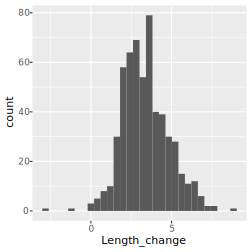
\includegraphics{insights_website_files/figure-latex/unnamed-chunk-143-4} \end{center}

\begin{Shaded}
\begin{Highlighting}[]
\KeywordTok{ggplot}\NormalTok{(dd, }\KeywordTok{aes}\NormalTok{(}\DataTypeTok{x=}\NormalTok{CI_change)) }\OperatorTok{+}
\StringTok{  }\KeywordTok{geom_histogram}\NormalTok{()}
\end{Highlighting}
\end{Shaded}

\begin{verbatim}
## `stat_bin()` using `bins = 30`. Pick better value with `binwidth`.
\end{verbatim}

\begin{verbatim}
## Warning: Removed 26 rows containing non-finite values (stat_bin).
\end{verbatim}

\begin{center}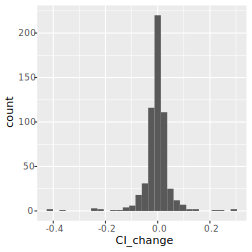
\includegraphics{insights_website_files/figure-latex/unnamed-chunk-143-5} \end{center}

\begin{Shaded}
\begin{Highlighting}[]
\NormalTok{dd <-}\StringTok{ }\NormalTok{dd }\OperatorTok
\StringTok{  }\KeywordTok{mutate}\NormalTok{(}\DataTypeTok{period=}\KeywordTok{cut}\NormalTok{(Lifespan, }\DataTypeTok{breaks=}\KeywordTok{c}\NormalTok{(}\OperatorTok{-}\DecValTok{1}\NormalTok{, }\DecValTok{20}\NormalTok{, }\DecValTok{60}\NormalTok{, }\DecValTok{106}\NormalTok{, }\DecValTok{120}\NormalTok{)))}
\end{Highlighting}
\end{Shaded}

\hypertarget{inspect-relationships}{%
\section{Inspect relationships}\label{inspect-relationships}}

``Male mortality risk was lowest on intermediate lipid intakes''.

\begin{Shaded}
\begin{Highlighting}[]
\NormalTok{dd }\OperatorTok\StringTok{ }\KeywordTok{filter}\NormalTok{(Sex}\OperatorTok{==}\StringTok{"Male"}\NormalTok{) }\OperatorTok
\KeywordTok{ggplot}\NormalTok{(}\KeywordTok{aes}\NormalTok{(}\DataTypeTok{x=}\NormalTok{Lipid, }\DataTypeTok{y=}\NormalTok{Lifespan, }\DataTypeTok{col=}\NormalTok{Prov_level)) }\OperatorTok{+}
\StringTok{  }\KeywordTok{geom_point}\NormalTok{(}\DataTypeTok{position =} \KeywordTok{position_jitterdodge}\NormalTok{(}\DataTypeTok{jitter.width=}\FloatTok{0.05}\NormalTok{)) }\OperatorTok{+}
\StringTok{  }\KeywordTok{facet_wrap}\NormalTok{(}\OperatorTok{~}\NormalTok{period, }\DataTypeTok{nrow=}\DecValTok{3}\NormalTok{)}
\end{Highlighting}
\end{Shaded}

\begin{center}\includegraphics{insights_website_files/figure-latex/unnamed-chunk-144-1} \end{center}

``Female risk was generally reduced by low protein intakes.''

\begin{Shaded}
\begin{Highlighting}[]
\NormalTok{dd }\OperatorTok\StringTok{ }\KeywordTok{filter}\NormalTok{(Sex}\OperatorTok{==}\StringTok{"Female"}\NormalTok{) }\OperatorTok
\KeywordTok{ggplot}\NormalTok{(}\KeywordTok{aes}\NormalTok{(}\DataTypeTok{x=}\NormalTok{Protein, }\DataTypeTok{y=}\NormalTok{Lifespan, }\DataTypeTok{col=}\NormalTok{Prov_level)) }\OperatorTok{+}
\StringTok{  }\KeywordTok{geom_point}\NormalTok{(}\DataTypeTok{position =} \KeywordTok{position_jitterdodge}\NormalTok{(}\DataTypeTok{jitter.width=}\FloatTok{0.05}\NormalTok{)) }\OperatorTok{+}
\StringTok{  }\KeywordTok{facet_wrap}\NormalTok{(}\OperatorTok{~}\NormalTok{period, }\DataTypeTok{nrow=}\DecValTok{3}\NormalTok{)}
\end{Highlighting}
\end{Shaded}

\begin{center}\includegraphics{insights_website_files/figure-latex/unnamed-chunk-145-1} \end{center}

``The effect of macronutrient intake on reproduction was similar between the sexes, with high protein intakes maximizing reproduction.''

\begin{Shaded}
\begin{Highlighting}[]
\NormalTok{dd }\OperatorTok\StringTok{ }\KeywordTok{filter}\NormalTok{(Sex}\OperatorTok{==}\StringTok{"Male"}\NormalTok{) }\OperatorTok
\KeywordTok{ggplot}\NormalTok{(}\KeywordTok{aes}\NormalTok{(}\DataTypeTok{x=}\NormalTok{Protein, }\DataTypeTok{y=}\NormalTok{Total_court, }\DataTypeTok{col=}\NormalTok{Prov_level)) }\OperatorTok{+}
\StringTok{  }\KeywordTok{geom_point}\NormalTok{(}\DataTypeTok{position =} \KeywordTok{position_jitterdodge}\NormalTok{(}\DataTypeTok{jitter.width=}\FloatTok{0.05}\NormalTok{))}
\end{Highlighting}
\end{Shaded}

\begin{verbatim}
## Warning: Removed 67 rows containing missing values (geom_point).
\end{verbatim}

\begin{center}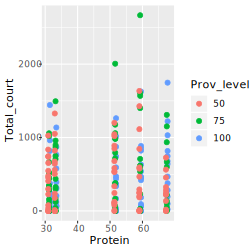
\includegraphics{insights_website_files/figure-latex/unnamed-chunk-146-1} \end{center}

\begin{Shaded}
\begin{Highlighting}[]
\NormalTok{dd }\OperatorTok\StringTok{ }\KeywordTok{filter}\NormalTok{(Sex}\OperatorTok{==}\StringTok{"Female"}\NormalTok{) }\OperatorTok
\KeywordTok{ggplot}\NormalTok{(}\KeywordTok{aes}\NormalTok{(}\DataTypeTok{x=}\NormalTok{Protein, }\DataTypeTok{y=}\NormalTok{Total_court, }\DataTypeTok{col=}\NormalTok{Prov_level)) }\OperatorTok{+}
\StringTok{  }\KeywordTok{geom_point}\NormalTok{(}\DataTypeTok{position =} \KeywordTok{position_jitterdodge}\NormalTok{(}\DataTypeTok{jitter.width=}\FloatTok{0.05}\NormalTok{))}
\end{Highlighting}
\end{Shaded}

\begin{verbatim}
## Warning: Removed 292 rows containing missing values (geom_point).
\end{verbatim}

\begin{center}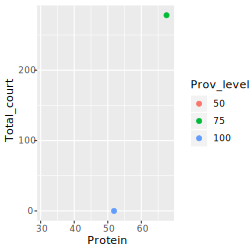
\includegraphics{insights_website_files/figure-latex/unnamed-chunk-146-2} \end{center}

\begin{Shaded}
\begin{Highlighting}[]
\NormalTok{dd }\OperatorTok\StringTok{ }\KeywordTok{filter}\NormalTok{(Sex}\OperatorTok{==}\StringTok{"Male"}\NormalTok{) }\OperatorTok
\KeywordTok{ggplot}\NormalTok{(}\KeywordTok{aes}\NormalTok{(}\DataTypeTok{x=}\NormalTok{Protein, }\DataTypeTok{y=}\NormalTok{Total_egg, }\DataTypeTok{col=}\NormalTok{Prov_level)) }\OperatorTok{+}
\StringTok{  }\KeywordTok{geom_point}\NormalTok{(}\DataTypeTok{position =} \KeywordTok{position_jitterdodge}\NormalTok{(}\DataTypeTok{jitter.width=}\FloatTok{0.05}\NormalTok{))}
\end{Highlighting}
\end{Shaded}

\begin{verbatim}
## Warning: Removed 288 rows containing missing values (geom_point).
\end{verbatim}

\begin{center}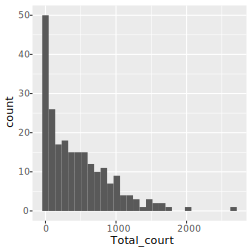
\includegraphics{insights_website_files/figure-latex/unnamed-chunk-147-1} \end{center}

\begin{Shaded}
\begin{Highlighting}[]
\NormalTok{dd }\OperatorTok\StringTok{ }\KeywordTok{filter}\NormalTok{(Sex}\OperatorTok{==}\StringTok{"Female"}\NormalTok{) }\OperatorTok
\KeywordTok{ggplot}\NormalTok{(}\KeywordTok{aes}\NormalTok{(}\DataTypeTok{x=}\NormalTok{Protein, }\DataTypeTok{y=}\NormalTok{Total_egg, }\DataTypeTok{col=}\NormalTok{Prov_level)) }\OperatorTok{+}
\StringTok{  }\KeywordTok{geom_point}\NormalTok{(}\DataTypeTok{position =} \KeywordTok{position_jitterdodge}\NormalTok{(}\DataTypeTok{jitter.width=}\FloatTok{0.2}\NormalTok{, }\DataTypeTok{dodge.width =} \DecValTok{5}\NormalTok{))}
\end{Highlighting}
\end{Shaded}

\begin{verbatim}
## Warning: position_jitterdodge requires non-overlapping x intervals
\end{verbatim}

\begin{verbatim}
## Warning: Removed 30 rows containing missing values (geom_point).
\end{verbatim}

\begin{center}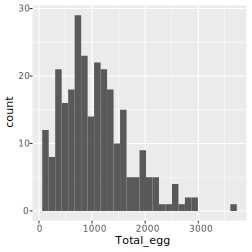
\includegraphics{insights_website_files/figure-latex/unnamed-chunk-147-2} \end{center}

\hypertarget{moatt-et-al-data-s1-mortality-data}{%
\section{Moatt et al Data S1 -- Mortality Data}\label{moatt-et-al-data-s1-mortality-data}}

\begin{itemize}
\tightlist
\item
  FID -- Unique ID for each individual.
\item
  Diet -- Diet Treatment (Diet P:L: 1 = 10.2:1, 2 = 4.6:1, 3 = 2.5:1, 4 = 8.5:1, 5 = 1.6:1).
\item
  Sex -- Sex of individual (M = male, F = female).
\item
  Size -- Size classification of individual (L = large, S = Small).
\item
  Level -- Provisioning level, values represent percentages of monthly ad libitum monitoring.
\item
  Total\_eaten -- Total pellet eaten in g from the start of the experiment.
\item
  Eaten\_wk -- Amount of pellet consumed that week (gweek-1).
\item
  P\_tot - Total protein eaten in g from the start of the experiment.
\item
  P2\_total -- P\_tot2 squared (i.e.~the total protein eaten squared).
\item
  P\_wk -- Amount of protein consumed that week (gweek-1).
\item
  P2\_wk -- P\_wk2 squared (i.e.~the weekly protein intake squared).
\item
  L\_tot - Total lipid eaten in g from the start of the experiment.
\item
  L2\_total -- L\_tot2 squared (i.e.~the total lipid eaten squared).
\item
  L\_wk -- Amount of lipid consumed that week (gweek-1).
\item
  L2\_wk -- L\_wk2 squared (i.e.~the weekly lipid intake squared).
\item
  Weight -- Weight of fish from last weighing (g).
\item
  Week\_F -- Experimental week.
\item
  Status -- Survival status (0= alive, 1 = Dead).
\item
  T\_group -- Time period of the experiment (see Fig. S1).
\item
  Initial\_weight -- Initial weight of individual at the start of the experiment.
\item
  ZP -- P\_wk z transformed (mean of 0 and standard deviation of 1).
\item
  ZP2 -- P2\_wk z transformed (mean of 0 and standard deviation of 1).
\item
  ZL -- L\_wk z transformed (mean of 0 and standard deviation of 1).
\item
  ZL2 -- L2\_wk z transformed (mean of 0 and standard deviation of 1).
\end{itemize}

\hypertarget{moatt-et-al-data-s5-courtship-data}{%
\section{Moatt et al Data S5 -- Courtship Data}\label{moatt-et-al-data-s5-courtship-data}}

\begin{itemize}
\tightlist
\item
  FID -- Unique ID for each individual.
\item
  Family -- Unique code for family group (i.e.~clutch of origin). Each clutch produced from a unique sire and dam.
\item
  Shelf\_stack -- Unique code for the stack and shelf of fish home tank.
\item
  Diet -- Diet Treatment (Diet P:L: 1 = 10.2:1, 2 = 4.6:1, 3 = 2.5:1, 4 = 8.5:1, 5 = 1.6:1).
\item
  Level -- Provisioning level, values represent percentages of monthly ad libitum monitoring.
\item
  Size -- Size classification of individual (L = large, S = Small).
\item
  Trial -- Number of trials that individual experienced.
\item
  Days\_breeding -- Length of breeding season for that individual.
\item
  P\_day -- Average protein intake per day during the breeding season (gday-1).
\item
  P2\_day -- P\_day2 squared (i.e.~daily protein intake squared).
\item
  L\_day - Average lipid intake per day during the breeding season (gday-1).
\item
  L2\_day -- L\_day2 squared (i.e.~daily lipid intake squared).
\item
  Mean\_react -- Mean reaction time across all trials for that individual.
\item
  Total\_ZZ -- Total number of zigzags across all trials.
\item
  Total\_leads -- Total number of leads across all trials.
\item
  Total\_court -- Total time courting across all trials.
\end{itemize}

\hypertarget{moatt-et-al-data-s6-eggs-data}{%
\section{Moatt et al Data S6 -- Eggs Data}\label{moatt-et-al-data-s6-eggs-data}}

\begin{itemize}
\tightlist
\item
  FID -- Unique ID for each individual.
\item
  Family -- Unique code for family group (i.e.~clutch of origin). Each clutch produced from a unique sire and dam.
\item
  Shelf\_stack -- Unique code for the stack and shelf of fish home tank.
\item
  Diet -- Diet Treatment (Diet P:L: 1 = 10.2:1, 2 = 4.6:1, 3 = 2.5:1, 4 = 8.5:1, 5 = 1.6:1).
\item
  Level -- Provisioning level, values represent percentages of monthly ad libitum monitoring.
\item
  Size -- Size classification of individual (L = large, S = Small).
\item
  P\_day -- Average protein intake per day during the breeding season (gday-1).
\item
  P2\_day -- P\_day2 squared (i.e.~daily protein intake squared).
\item
  L\_day - Average lipid intake per day during the breeding season (gday-1).
\item
  L2\_day -- L\_day2 squared (i.e.~daily lipid intake squared).
\item
  Days\_breeding -- Length of breeding season for that individual.
\item
  Number\_clutches -- Number of clutches produced by that individual.
\item
  Mean\_number -- Mean number of eggs per clutch.
\item
  Total\_egg -- Total number of eggs produced.
\end{itemize}

\hypertarget{moatt-et-al-data-s15-length-weight-and-condition-index-data}{%
\section{Moatt et al Data S15 -- Length, Weight and Condition Index Data}\label{moatt-et-al-data-s15-length-weight-and-condition-index-data}}

\begin{itemize}
\tightlist
\item
  FID -- Unique ID for each individual.
\item
  StackShelf -- Unique code for the stack and shelf of fish home tank.
\item
  Sex -- Sex of individual (M = male, F = female).
\item
  Diet -- Diet Treatment (Diet P:L: 1 = 10.2:1, 2 = 4.6:1, 3 = 2.5:1, 4 = 8.5:1, 5 = 1.6:1).
\item
  Level -- Provisioning level, values represent percentages of monthly ad libitum monitoring.
\item
  Size -- Size classification of individual (L = large, S = Small).
\item
  Batch -- Weighing batch. NB Batch 1 is prior to diet treatments therefore has no corresponding values for protein and lipid intake.
\item
  P\_day -- Average protein intake per day during the breeding season (gday-1).
\item
  P2\_day -- P\_day2 squared (i.e.~daily protein intake squared).
\item
  L\_day - Average lipid intake per day during the breeding season (gday-1).
\item
  L2\_day -- L\_day2 squared (i.e.~daily lipid intake squared).
\item
  ZP -- Daily protein intake z transformed (mean of 0 and standard deviation of 1), calculated for each sex independently.
\item
  ZP2 -- Daily protein intake squared, z transformed (mean of 0 and standard deviation of 1), calculated for each sex independently.
\item
  ZL -- Daily lipid intake z transformed (mean of 0 and standard deviation of 1), calculated for each sex independently.
\item
  ZL2 -- Daily lipid intake squared, z transformed (mean of 0 and standard deviation of 1), calculated for each sex independently.
\item
  Ln -- Length of individual in mm.
\item
  Wt -- Weight of individual in g.
\item
  CI -- Condition Index for each individual.
\end{itemize}

\hypertarget{summing-up}{%
\chapter{Summing up}\label{summing-up}}

\bibliography{book.bib,packages.bib}

\backmatter
\printindex

\end{document}
